\documentclass[]{book}
\usepackage{lmodern}
\usepackage{amssymb,amsmath}
\usepackage{ifxetex,ifluatex}
\usepackage{fixltx2e} % provides \textsubscript
\ifnum 0\ifxetex 1\fi\ifluatex 1\fi=0 % if pdftex
  \usepackage[T1]{fontenc}
  \usepackage[utf8]{inputenc}
\else % if luatex or xelatex
  \ifxetex
    \usepackage{mathspec}
  \else
    \usepackage{fontspec}
  \fi
  \defaultfontfeatures{Ligatures=TeX,Scale=MatchLowercase}
\fi
% use upquote if available, for straight quotes in verbatim environments
\IfFileExists{upquote.sty}{\usepackage{upquote}}{}
% use microtype if available
\IfFileExists{microtype.sty}{%
\usepackage{microtype}
\UseMicrotypeSet[protrusion]{basicmath} % disable protrusion for tt fonts
}{}
\usepackage[margin=1in]{geometry}
\usepackage{hyperref}
\hypersetup{unicode=true,
            pdftitle={Longitudinal Analysis},
            pdfauthor={Richard White},
            pdfborder={0 0 0},
            breaklinks=true}
\urlstyle{same}  % don't use monospace font for urls
\usepackage{natbib}
\bibliographystyle{apalike}
\usepackage{color}
\usepackage{fancyvrb}
\newcommand{\VerbBar}{|}
\newcommand{\VERB}{\Verb[commandchars=\\\{\}]}
\DefineVerbatimEnvironment{Highlighting}{Verbatim}{commandchars=\\\{\}}
% Add ',fontsize=\small' for more characters per line
\usepackage{framed}
\definecolor{shadecolor}{RGB}{248,248,248}
\newenvironment{Shaded}{\begin{snugshade}}{\end{snugshade}}
\newcommand{\KeywordTok}[1]{\textcolor[rgb]{0.13,0.29,0.53}{\textbf{#1}}}
\newcommand{\DataTypeTok}[1]{\textcolor[rgb]{0.13,0.29,0.53}{#1}}
\newcommand{\DecValTok}[1]{\textcolor[rgb]{0.00,0.00,0.81}{#1}}
\newcommand{\BaseNTok}[1]{\textcolor[rgb]{0.00,0.00,0.81}{#1}}
\newcommand{\FloatTok}[1]{\textcolor[rgb]{0.00,0.00,0.81}{#1}}
\newcommand{\ConstantTok}[1]{\textcolor[rgb]{0.00,0.00,0.00}{#1}}
\newcommand{\CharTok}[1]{\textcolor[rgb]{0.31,0.60,0.02}{#1}}
\newcommand{\SpecialCharTok}[1]{\textcolor[rgb]{0.00,0.00,0.00}{#1}}
\newcommand{\StringTok}[1]{\textcolor[rgb]{0.31,0.60,0.02}{#1}}
\newcommand{\VerbatimStringTok}[1]{\textcolor[rgb]{0.31,0.60,0.02}{#1}}
\newcommand{\SpecialStringTok}[1]{\textcolor[rgb]{0.31,0.60,0.02}{#1}}
\newcommand{\ImportTok}[1]{#1}
\newcommand{\CommentTok}[1]{\textcolor[rgb]{0.56,0.35,0.01}{\textit{#1}}}
\newcommand{\DocumentationTok}[1]{\textcolor[rgb]{0.56,0.35,0.01}{\textbf{\textit{#1}}}}
\newcommand{\AnnotationTok}[1]{\textcolor[rgb]{0.56,0.35,0.01}{\textbf{\textit{#1}}}}
\newcommand{\CommentVarTok}[1]{\textcolor[rgb]{0.56,0.35,0.01}{\textbf{\textit{#1}}}}
\newcommand{\OtherTok}[1]{\textcolor[rgb]{0.56,0.35,0.01}{#1}}
\newcommand{\FunctionTok}[1]{\textcolor[rgb]{0.00,0.00,0.00}{#1}}
\newcommand{\VariableTok}[1]{\textcolor[rgb]{0.00,0.00,0.00}{#1}}
\newcommand{\ControlFlowTok}[1]{\textcolor[rgb]{0.13,0.29,0.53}{\textbf{#1}}}
\newcommand{\OperatorTok}[1]{\textcolor[rgb]{0.81,0.36,0.00}{\textbf{#1}}}
\newcommand{\BuiltInTok}[1]{#1}
\newcommand{\ExtensionTok}[1]{#1}
\newcommand{\PreprocessorTok}[1]{\textcolor[rgb]{0.56,0.35,0.01}{\textit{#1}}}
\newcommand{\AttributeTok}[1]{\textcolor[rgb]{0.77,0.63,0.00}{#1}}
\newcommand{\RegionMarkerTok}[1]{#1}
\newcommand{\InformationTok}[1]{\textcolor[rgb]{0.56,0.35,0.01}{\textbf{\textit{#1}}}}
\newcommand{\WarningTok}[1]{\textcolor[rgb]{0.56,0.35,0.01}{\textbf{\textit{#1}}}}
\newcommand{\AlertTok}[1]{\textcolor[rgb]{0.94,0.16,0.16}{#1}}
\newcommand{\ErrorTok}[1]{\textcolor[rgb]{0.64,0.00,0.00}{\textbf{#1}}}
\newcommand{\NormalTok}[1]{#1}
\usepackage{longtable,booktabs}
\usepackage{graphicx,grffile}
\makeatletter
\def\maxwidth{\ifdim\Gin@nat@width>\linewidth\linewidth\else\Gin@nat@width\fi}
\def\maxheight{\ifdim\Gin@nat@height>\textheight\textheight\else\Gin@nat@height\fi}
\makeatother
% Scale images if necessary, so that they will not overflow the page
% margins by default, and it is still possible to overwrite the defaults
% using explicit options in \includegraphics[width, height, ...]{}
\setkeys{Gin}{width=\maxwidth,height=\maxheight,keepaspectratio}
\IfFileExists{parskip.sty}{%
\usepackage{parskip}
}{% else
\setlength{\parindent}{0pt}
\setlength{\parskip}{6pt plus 2pt minus 1pt}
}
\setlength{\emergencystretch}{3em}  % prevent overfull lines
\providecommand{\tightlist}{%
  \setlength{\itemsep}{0pt}\setlength{\parskip}{0pt}}
\setcounter{secnumdepth}{5}
% Redefines (sub)paragraphs to behave more like sections
\ifx\paragraph\undefined\else
\let\oldparagraph\paragraph
\renewcommand{\paragraph}[1]{\oldparagraph{#1}\mbox{}}
\fi
\ifx\subparagraph\undefined\else
\let\oldsubparagraph\subparagraph
\renewcommand{\subparagraph}[1]{\oldsubparagraph{#1}\mbox{}}
\fi

%%% Use protect on footnotes to avoid problems with footnotes in titles
\let\rmarkdownfootnote\footnote%
\def\footnote{\protect\rmarkdownfootnote}

%%% Change title format to be more compact
\usepackage{titling}

% Create subtitle command for use in maketitle
\newcommand{\subtitle}[1]{
  \posttitle{
    \begin{center}\large#1\end{center}
    }
}

\setlength{\droptitle}{-2em}

  \title{Longitudinal Analysis}
    \pretitle{\vspace{\droptitle}\centering\huge}
  \posttitle{\par}
    \author{Richard White}
    \preauthor{\centering\large\emph}
  \postauthor{\par}
      \predate{\centering\large\emph}
  \postdate{\par}
    \date{2018-11-02}

\usepackage{booktabs}

\begin{document}
\maketitle

{
\setcounter{tocdepth}{1}
\tableofcontents
}
\chapter{Syllabus}\label{syllabus}

\textbf{Instructor:} Richard White
{[}\href{mailto:richard.white@fhi.no}{\nolinkurl{richard.white@fhi.no}}{]}

\textbf{Time:} 09:30 - 15:00, 18th September 2017

\textbf{Location:} Main auditorium, L8, Lindern Campus,
Folkehelseinstittutet, Oslo

\textbf{Language:} English

\textbf{Format and Procedures}

09:00 - 10:00: Lecture 1

10:00 - 10:10: Break

10:10 - 11:10: Lecture 2

10:10 - 10:15: Break

11:15 - 11:45: Examples from FHI

\textbf{Description}

This course will provide a basic overview of general statistical
methodology that can be useful in the areas of infectious diseases,
environmental medicine, and labwork. By the end of this course, students
will be able to identify appropriate statistical methods for a variety
of circumstances.

This course will \textbf{not} teach students how to implement these
statistical methods, as there is not sufficient time. The aim of this
course is to enable the student to identify which methods are required
for their study, allowing the student to identify their needs for
subsequent methods courses, self-learning, or external help.

You should register for this course if you are one of the following:

\begin{itemize}
\tightlist
\item
  Have experience with applying statistical methods, but are sometimes
  confused or uncertain as to whether or not you have selected the
  correct method.
\item
  Do not have experience with applying statistical methods, and would
  like to get an overview over which methods are applicable for your
  projects so that you can then undertake further studies in these
  areas.
\end{itemize}

\textbf{Lecture 1}

\begin{enumerate}
\def\labelenumi{\arabic{enumi}.}
\tightlist
\item
  Identifying continuous, categorical, count, and censored variables
\item
  Identifying exposure and outcome variables
\item
  Identifying when t-tests (paired and unpaired) should be used
\item
  Identifying when non-parametric t-test equivalents should be used
\item
  Identifying when ANOVA should be used
\item
  Identifying when linear regression should be used
\item
  Identifying the similarities between t-tests, ANOVA, and regression
\item
  Identifying when logistic regression models should be used
\item
  Identifying when Poisson/negative binomial and cox regression models
  should be used
\item
  Identifying when chi-squared/fisher's exact test should be used
\end{enumerate}

\textbf{Lecture 2}

\begin{enumerate}
\def\labelenumi{\arabic{enumi}.}
\tightlist
\item
  Identifying when data does not have any dependencies (i.e.~all
  observations are independent of each other) versus when data has
  complicated dependencies (i.e.~longitudinal data, matched data,
  multiple cohorts)
\item
  Identifying when mixed effects regression models should be used
\item
  Identifying when conditional logistic regression models should be used
\item
  (TBD) Understanding the different imputation methods used when lab
  data is below the limit of detection (LOD)
\item
  (TBD) Understanding the best practices for data files and project
  folders
\end{enumerate}

\textbf{Prerequisites}

To participate in this course it is recommended that you have some
experience with either research or data.

\textbf{Additional information}

For the last 30 minutes of the course we will be going through examples
of analyses performed at FHI and identifying which statistical methods
are appropriate. If you would like your analysis to be featured/included
in this section, please send an email to
\href{mailto:richard.white@fhi.no}{\nolinkurl{richard.white@fhi.no}}
briefly describing your problem.

\chapter{Reference}\label{reference}

\section{Scope of this course}\label{scope-of-this-course}

When dealing with longitudinal data, there are two kinds of analyses
that can be performed.

``Time series'' analyses generally deal with one variable. The aim is to
then predict the future only using the previous observations. A common
example would be to predict tomorrow's temperature, using today's and
yesterday's temperature as exposures. We will not be focusing on these
kinds of analyses in this course.

``Regression analyses'' are very similar to ordinary regressions that
you have been working with for many years. The only difference is that
they have more advanced data structures that your current methods cannot
handle. For example, if you want to see how the number of tuberculosis
patients (outcome) is affected by the number of immigrants to Norway
(exposure) over a 20 year period, then the number of patients in each
year might be associated with each other, which might break assumptions
of the regression models that you normally use (independent residuals).
To account for the advanced structure of the data (correlation between
different years) we will use more advanced regression techniques. This
is what we will be focusing on in this course.

To recap: this course will let you run ``normal regressions'' in
situations where the data structure would ordinarily prohibit you from
running regression models. These situations mostly pertain to clusters
of correlated data.

\newpage

\section{Introduction}\label{introduction}

There are two important definitions in this course:

\begin{itemize}
\tightlist
\item
  Panel data
\item
  Autocorrelation
\end{itemize}

Panel data is a set of data with measurements repeated at equally spaced
points. For example, weight data recorded every day, or every week, or
every year would be considered panel data. A person who records three
weight measurements randomly in 2018 would not be considered panel data.

When you have panel data, autocorrelation is the correlation between
subsequent observations. For example, if you have daily observations,
then the 1 day autocorrelation is the correlation between observations 1
day apart, and likewise the 2 day autocorrelation is the correlation
between observations 2 days apart.

In this course we will consider 5 scenarios where we have multiple
observations for each geographical area:

\begin{itemize}
\tightlist
\item
  Panel data: One geographical area, no autocorrelation
\item
  Panel data: One geographical area, with autocorrelation
\item
  Not panel data: Multiple geographical areas
\item
  Panel data: Multiple geographical areas, no autocorrelation
\item
  Panel data: Multiple geographical areas, with autocorrelation
\end{itemize}

Note, the following scenario can be covered by standard regression
models:

\begin{itemize}
\tightlist
\item
  Multiple geographical areas, one time point/observation per
  geographical area
\end{itemize}

\newpage

\section{Method summary}\label{method-summary}

\subsection{Panel data: One geographical area, no
autocorrelation}\label{panel-data-one-geographical-area-no-autocorrelation}

\begin{verbatim}
// STATA CODE
glm y yearminus2000 dailyrainfall cos365 sin365, family(poisson)
\end{verbatim}

\begin{Shaded}
\begin{Highlighting}[]
\CommentTok{# R CODE}
\NormalTok{fit1 <-}\StringTok{ }\KeywordTok{glm}\NormalTok{(y}\OperatorTok{~}\NormalTok{yearMinus2000 }\OperatorTok{+}\StringTok{ }\NormalTok{dailyrainfall }\OperatorTok{+}\StringTok{ }\NormalTok{sin365 }\OperatorTok{+}\StringTok{ }\NormalTok{cos365, }\DataTypeTok{data=}\NormalTok{d, }\DataTypeTok{family=}\KeywordTok{poisson}\NormalTok{())}
\KeywordTok{residuals}\NormalTok{(fit1, }\DataTypeTok{type =} \StringTok{"response"}\NormalTok{)}
\end{Highlighting}
\end{Shaded}

\subsection{Panel data: One geographical area, with
autocorrelation}\label{panel-data-one-geographical-area-with-autocorrelation}

\begin{verbatim}
// STATA CODE
glm y yearminus2000 cos365 sin365, family(poisson) vce(robust)
\end{verbatim}

\begin{Shaded}
\begin{Highlighting}[]
\CommentTok{# R CODE}
\NormalTok{fit <-}\StringTok{ }\NormalTok{MASS}\OperatorTok{::}\KeywordTok{glmmPQL}\NormalTok{(y}\OperatorTok{~}\NormalTok{yearMinus2000}\OperatorTok{+}\NormalTok{sin365 }\OperatorTok{+}\StringTok{ }\NormalTok{cos365, }\DataTypeTok{random =} \OperatorTok{~}\StringTok{ }\DecValTok{1} \OperatorTok{|}\StringTok{ }\NormalTok{ID,}
                \DataTypeTok{family =}\NormalTok{ poisson, }\DataTypeTok{data =}\NormalTok{ d,}
                \DataTypeTok{correlation=}\NormalTok{nlme}\OperatorTok{::}\KeywordTok{corAR1}\NormalTok{(}\DataTypeTok{form=}\OperatorTok{~}\NormalTok{dayOfSeries}\OperatorTok{|}\NormalTok{ID))}
\NormalTok{r <-}\StringTok{ }\KeywordTok{residuals}\NormalTok{(fit1, }\DataTypeTok{type =} \StringTok{"normalized"}\NormalTok{)}
\KeywordTok{pacf}\NormalTok{(r)}
\end{Highlighting}
\end{Shaded}

\subsection{Not panel data: Multiple geographical
areas}\label{not-panel-data-multiple-geographical-areas}

\begin{verbatim}
// STATA CODE
meglm y x yearMinus2000 || fylke:, family(poisson)
\end{verbatim}

\begin{Shaded}
\begin{Highlighting}[]
\CommentTok{# R CODE}
\NormalTok{fit <-}\StringTok{ }\NormalTok{lme4}\OperatorTok{::}\KeywordTok{glmer}\NormalTok{(y}\OperatorTok{~}\NormalTok{x }\OperatorTok{+}\StringTok{ }\NormalTok{yearMinus2000 }\OperatorTok{+}\StringTok{ }\NormalTok{(}\DecValTok{1}\OperatorTok{|}\NormalTok{fylke),}\DataTypeTok{data=}\NormalTok{d,}\DataTypeTok{family=}\KeywordTok{poisson}\NormalTok{())}
\end{Highlighting}
\end{Shaded}

\subsection{Panel data: Multiple geographical areas, no
autocorrelation}\label{panel-data-multiple-geographical-areas-no-autocorrelation}

\begin{verbatim}
// STATA CODE
meglm y yearminus2000 cos365 sin365 || fylke:, family(poisson)
\end{verbatim}

\begin{Shaded}
\begin{Highlighting}[]
\CommentTok{# R CODE}
\NormalTok{fit <-}\StringTok{ }\NormalTok{MASS}\OperatorTok{::}\KeywordTok{glmmPQL}\NormalTok{(y}\OperatorTok{~}\NormalTok{yearMinus2000}\OperatorTok{+}\NormalTok{sin365 }\OperatorTok{+}\StringTok{ }\NormalTok{cos365, }\DataTypeTok{random =} \OperatorTok{~}\StringTok{ }\DecValTok{1} \OperatorTok{|}\StringTok{ }\NormalTok{fylke,}
                \DataTypeTok{family =}\NormalTok{ poisson, }\DataTypeTok{data =}\NormalTok{ d)}
\NormalTok{r <-}\StringTok{ }\KeywordTok{residuals}\NormalTok{(fit1, }\DataTypeTok{type =} \StringTok{"normalized"}\NormalTok{)}
\KeywordTok{pacf}\NormalTok{(r)}
\end{Highlighting}
\end{Shaded}

\subsection{Panel data: Multiple geographical areas, with
autocorrelation}\label{panel-data-multiple-geographical-areas-with-autocorrelation}

\begin{verbatim}
// STATA CODE
meglm y yearminus2000 cos365 sin365 || fylke:, family(poisson) vce(robust)
\end{verbatim}

\begin{Shaded}
\begin{Highlighting}[]
\CommentTok{# R CODE}
\NormalTok{fit <-}\StringTok{ }\NormalTok{MASS}\OperatorTok{::}\KeywordTok{glmmPQL}\NormalTok{(y}\OperatorTok{~}\NormalTok{yearMinus2000}\OperatorTok{+}\NormalTok{sin365 }\OperatorTok{+}\StringTok{ }\NormalTok{cos365, }\DataTypeTok{random =} \OperatorTok{~}\StringTok{ }\DecValTok{1} \OperatorTok{|}\StringTok{ }\NormalTok{fylke,}
                \DataTypeTok{family =}\NormalTok{ poisson, }\DataTypeTok{data =}\NormalTok{ d,}
                \DataTypeTok{correlation=}\NormalTok{nlme}\OperatorTok{::}\KeywordTok{corAR1}\NormalTok{(}\DataTypeTok{form=}\OperatorTok{~}\NormalTok{dayOfSeries}\OperatorTok{|}\NormalTok{fylke))}
\NormalTok{r <-}\StringTok{ }\KeywordTok{residuals}\NormalTok{(fit1, }\DataTypeTok{type =} \StringTok{"normalized"}\NormalTok{)}
\KeywordTok{pacf}\NormalTok{(r)}
\end{Highlighting}
\end{Shaded}

\newpage

\section{Identifying your scenario}\label{identifying-your-scenario}

\subsection{Step 1: Do you have panel
data?}\label{step-1-do-you-have-panel-data}

This step should be fairly simple. If your data has equally spaced time
intervals between them, you have panel data.

\subsection{Step 2: Do you have multiple geographical
areas?}\label{step-2-do-you-have-multiple-geographical-areas}

Again, fairly simple, just look at your data.

\subsection{Step 3: Do you have
autocorrelation?}\label{step-3-do-you-have-autocorrelation}

Firstly, you must run a model pretending that you do not have
autocorrelation.

You then inspect the residuals from the model and see if autocorrelation
exists. This is done with two statistical procedures: \texttt{pacf} (for
\texttt{autoregressive\ models}, the most common type of
autocorrelation), and \texttt{acf} (for
\texttt{moving\ average\ models}, a less common type of
autocorrelation).

\newpage 

\subsection{AR(1) data}\label{ar1-data}

\begin{Shaded}
\begin{Highlighting}[]
\NormalTok{y <-}\StringTok{ }\KeywordTok{round}\NormalTok{(}\KeywordTok{as.numeric}\NormalTok{(}\KeywordTok{arima.sim}\NormalTok{(}\DataTypeTok{model=}\KeywordTok{list}\NormalTok{(}\StringTok{"ar"}\NormalTok{=}\KeywordTok{c}\NormalTok{(}\FloatTok{0.5}\NormalTok{)), }\DataTypeTok{rand.gen =}\NormalTok{ rnorm, }\DataTypeTok{n=}\DecValTok{1000}\NormalTok{)))}
\end{Highlighting}
\end{Shaded}

With \texttt{autoregressive} data, a \texttt{pacf} plot contains a
number of sharp significant lines, indicating how many subsequent
observations have autocorrelation. i.e.~if one line is significant, it
means that each observation is only correlated with its preceeding
observation (\texttt{AR(1)}). If two lines are significant, it means
that each observation is correlated with its two preceeding observations
(\texttt{AR(2)}). The following plot represents \texttt{AR(1)} data.

\begin{Shaded}
\begin{Highlighting}[]
\KeywordTok{pacf}\NormalTok{(y)}
\end{Highlighting}
\end{Shaded}

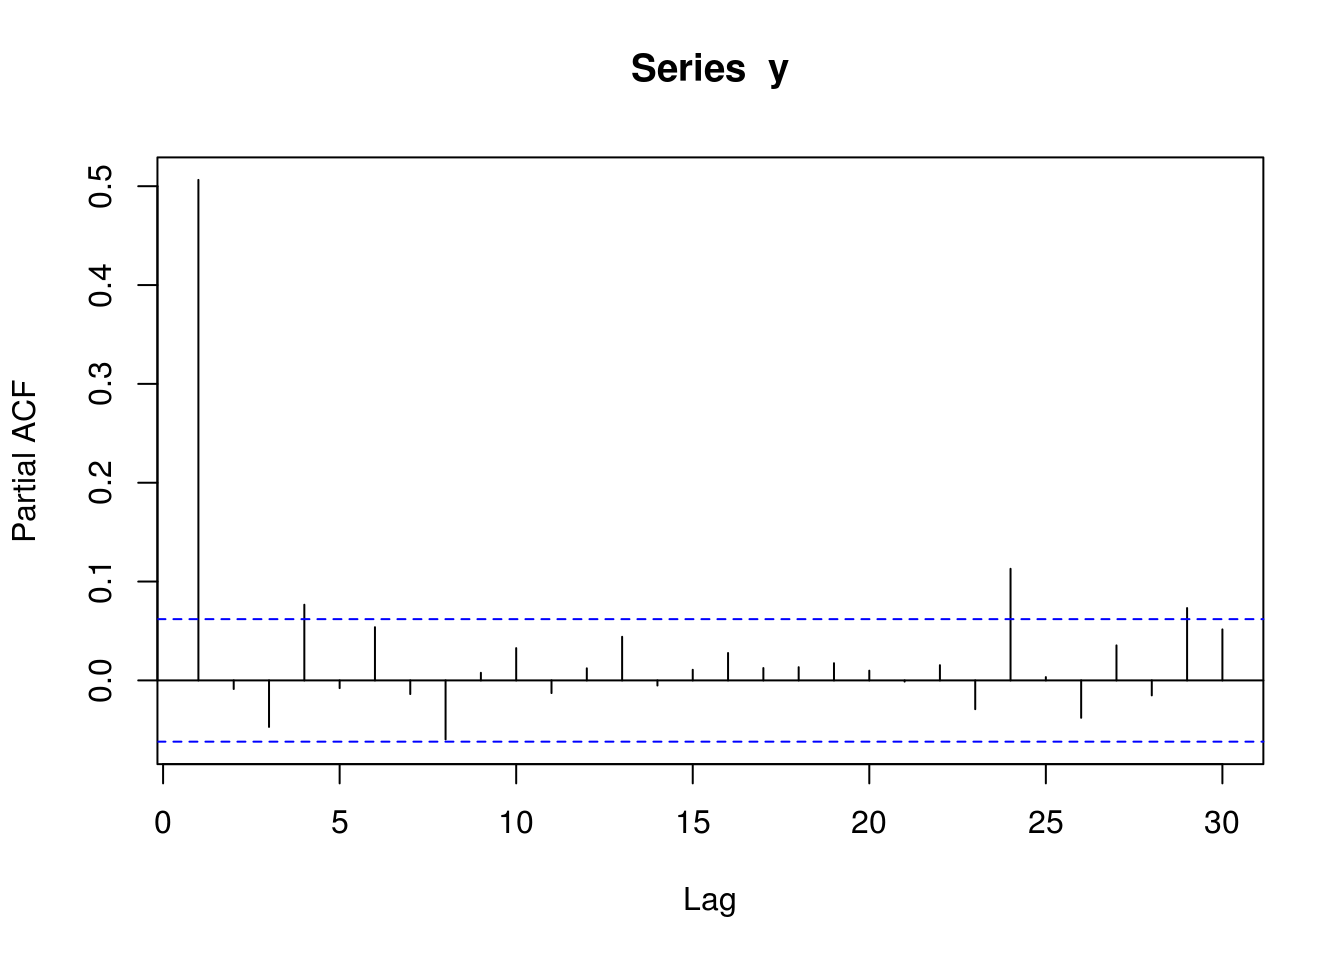
\includegraphics{website_files/figure-latex/unnamed-chunk-7-1.pdf}

\newpage

With \texttt{autoregressive} data, an \texttt{acf} plot contains a
number of decreasing lines. The following \texttt{acf} plot represents
some sort of \texttt{AR} data. Note that the \texttt{acf} plot displays
\texttt{lag\ 0} (which is pointless and can be ignored), while the
\texttt{pacf} plot does not.

\begin{Shaded}
\begin{Highlighting}[]
\KeywordTok{acf}\NormalTok{(y)}
\end{Highlighting}
\end{Shaded}

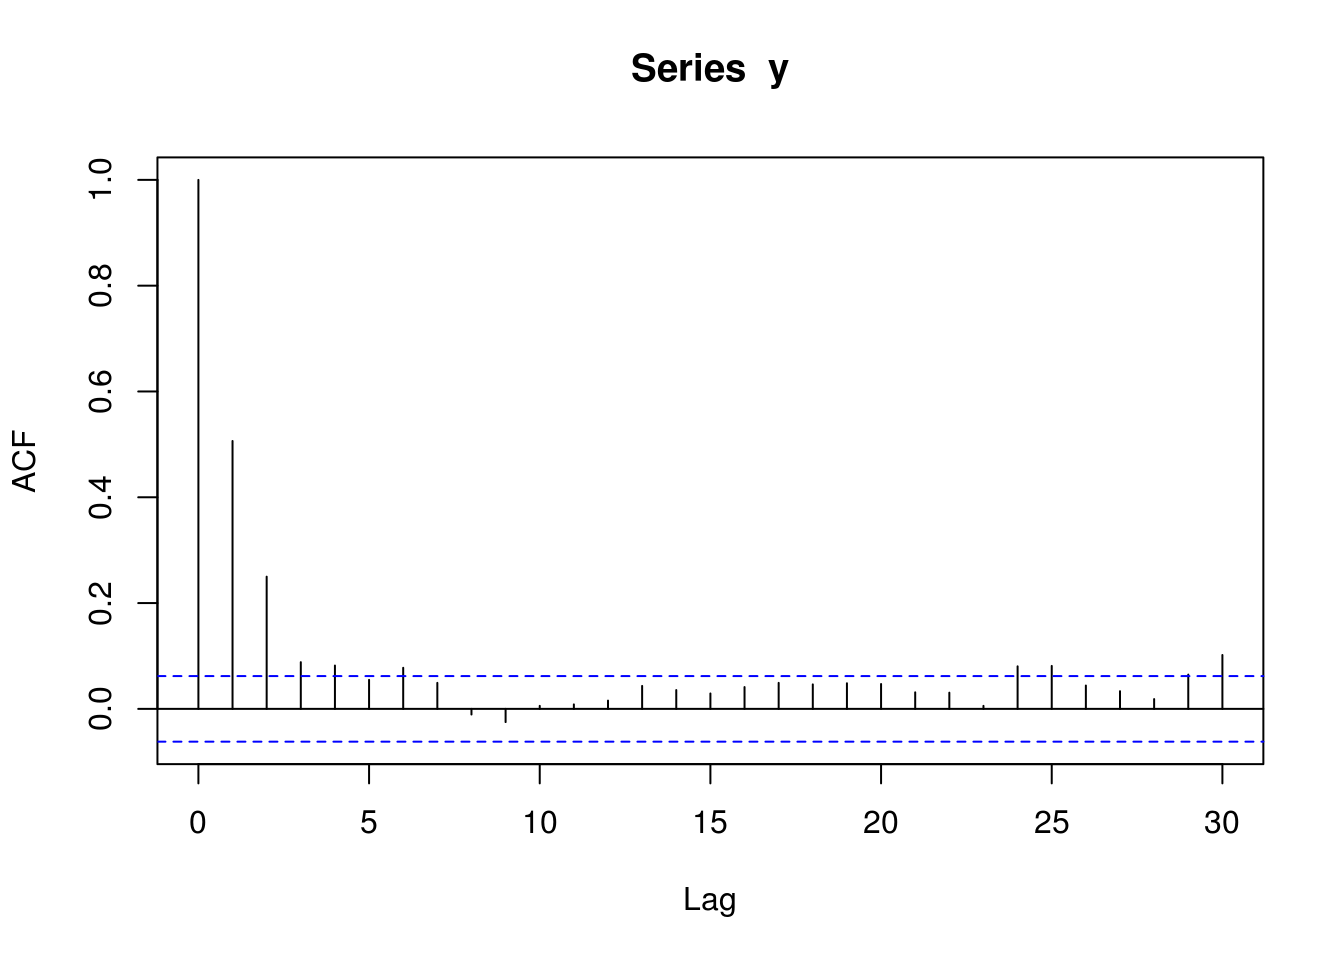
\includegraphics{website_files/figure-latex/unnamed-chunk-8-1.pdf}

\newpage 

\subsection{AR(2) data}\label{ar2-data}

\begin{Shaded}
\begin{Highlighting}[]
\NormalTok{y <-}\StringTok{ }\KeywordTok{round}\NormalTok{(}\KeywordTok{as.numeric}\NormalTok{(}\KeywordTok{arima.sim}\NormalTok{(}\DataTypeTok{model=}\KeywordTok{list}\NormalTok{(}\StringTok{"ar"}\NormalTok{=}\KeywordTok{c}\NormalTok{(}\FloatTok{0.5}\NormalTok{,}\FloatTok{0.4}\NormalTok{)), }\DataTypeTok{rand.gen =}\NormalTok{ rnorm, }\DataTypeTok{n=}\DecValTok{1000}\NormalTok{)))}
\end{Highlighting}
\end{Shaded}

The following \texttt{pacf} plot represents \texttt{AR(2)} data. This
means that each observation is correlated with its two preceeding
observations (\texttt{AR(2)}).

\begin{Shaded}
\begin{Highlighting}[]
\KeywordTok{pacf}\NormalTok{(y)}
\end{Highlighting}
\end{Shaded}

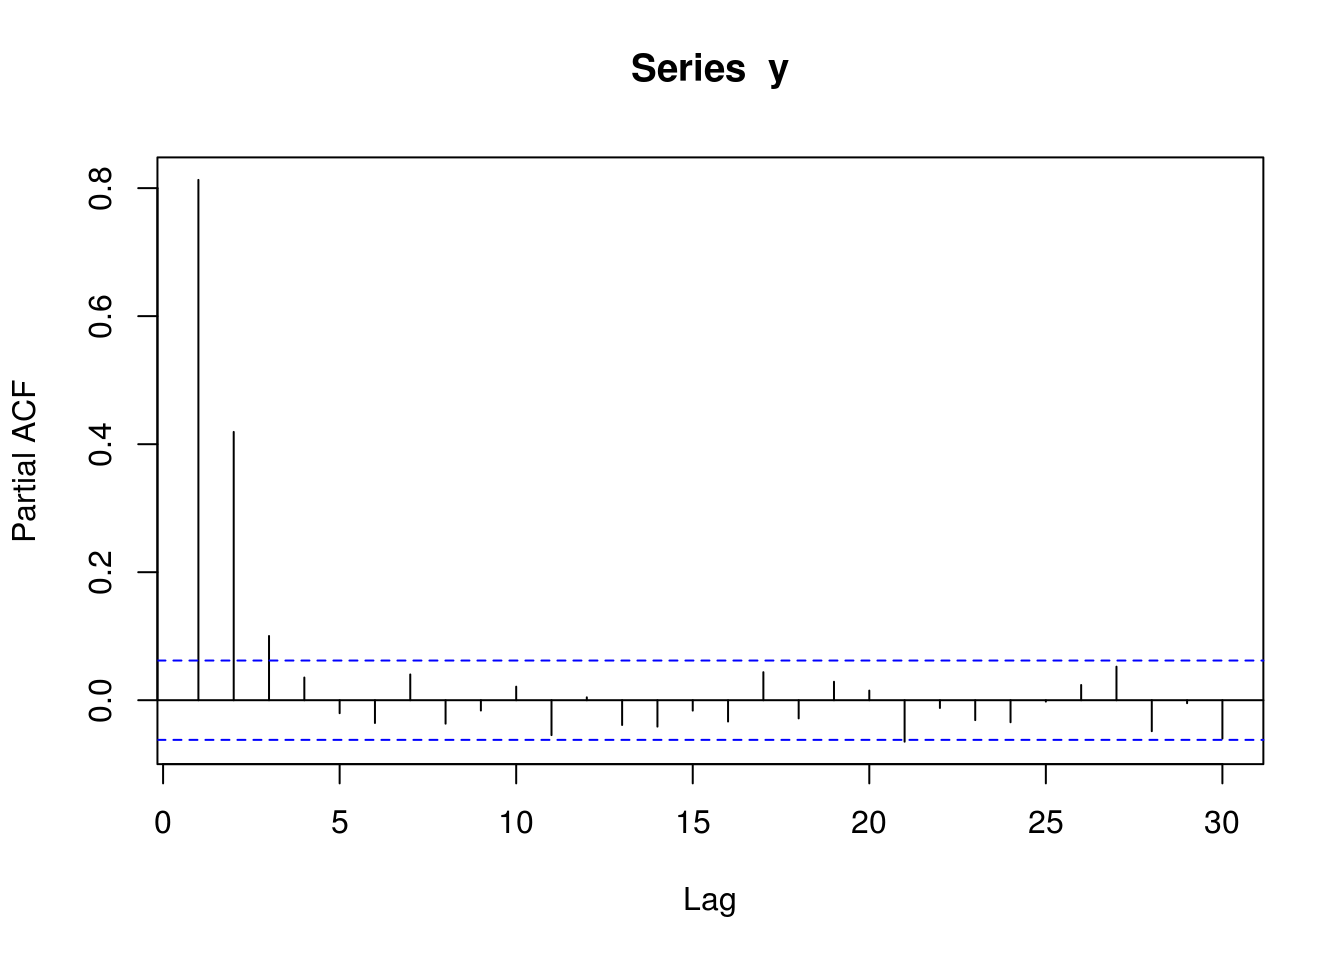
\includegraphics{website_files/figure-latex/unnamed-chunk-10-1.pdf}

\newpage

The following \texttt{acf} plot represents some sort of \texttt{AR}
data:

\begin{Shaded}
\begin{Highlighting}[]
\KeywordTok{acf}\NormalTok{(y)}
\end{Highlighting}
\end{Shaded}

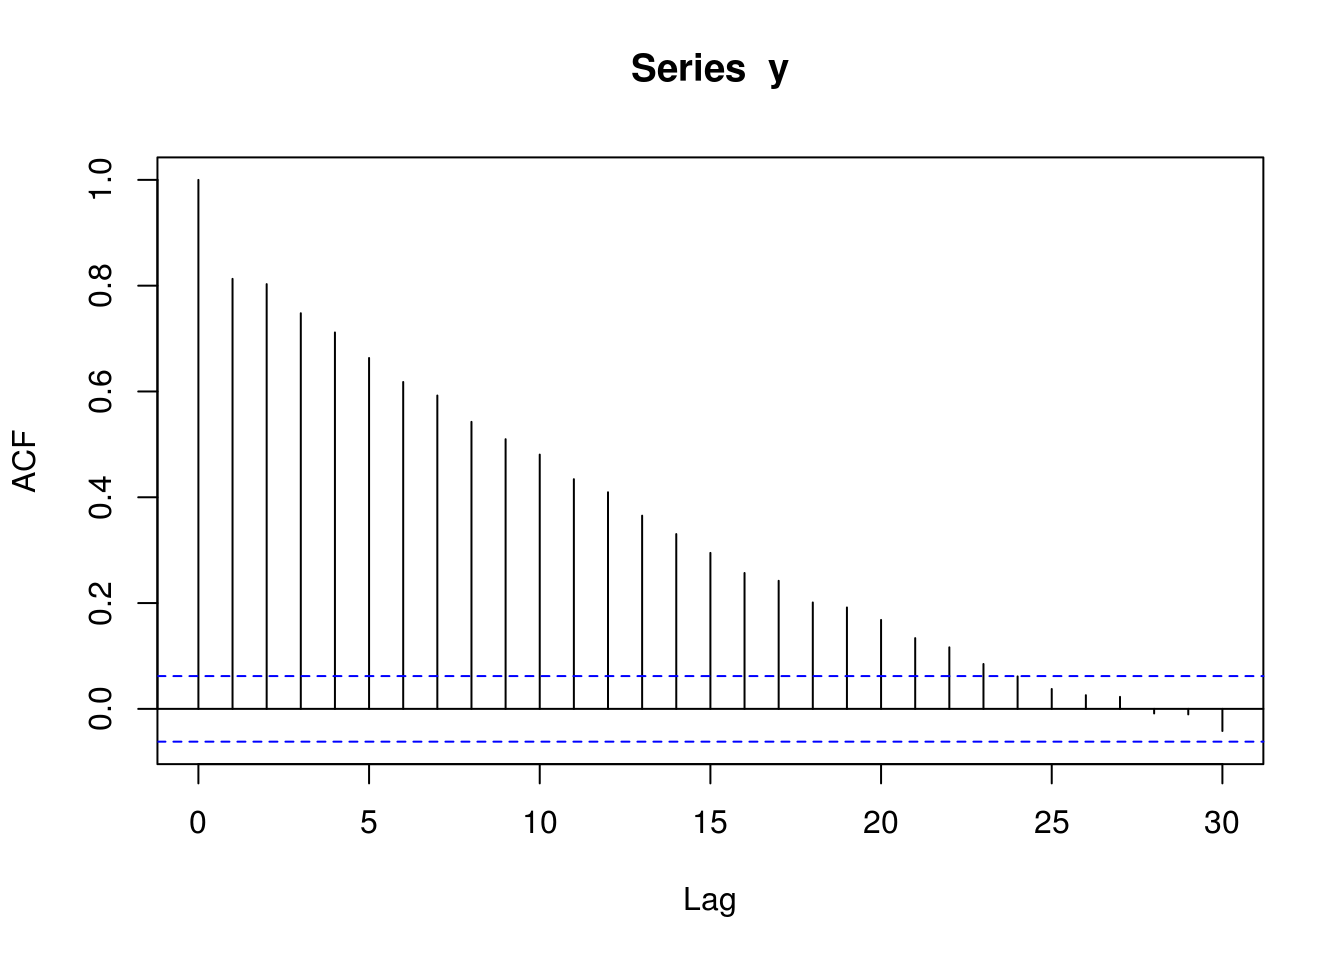
\includegraphics{website_files/figure-latex/unnamed-chunk-11-1.pdf}

\newpage 

\subsection{MA(1) data}\label{ma1-data}

\begin{Shaded}
\begin{Highlighting}[]
\NormalTok{y <-}\StringTok{ }\KeywordTok{round}\NormalTok{(}\KeywordTok{as.numeric}\NormalTok{(}\KeywordTok{arima.sim}\NormalTok{(}\DataTypeTok{model=}\KeywordTok{list}\NormalTok{(}\StringTok{"ma"}\NormalTok{=}\KeywordTok{c}\NormalTok{(}\FloatTok{0.9}\NormalTok{)), }\DataTypeTok{rand.gen =}\NormalTok{ rnorm, }\DataTypeTok{n=}\DecValTok{1000}\NormalTok{)))}
\end{Highlighting}
\end{Shaded}

With \texttt{moving\ average} data, a \texttt{pacf} plot contains a
number of decreasing lines. The following \texttt{pacf} plot represents
some sort of \texttt{MA} data.:

\begin{Shaded}
\begin{Highlighting}[]
\KeywordTok{pacf}\NormalTok{(y)}
\end{Highlighting}
\end{Shaded}

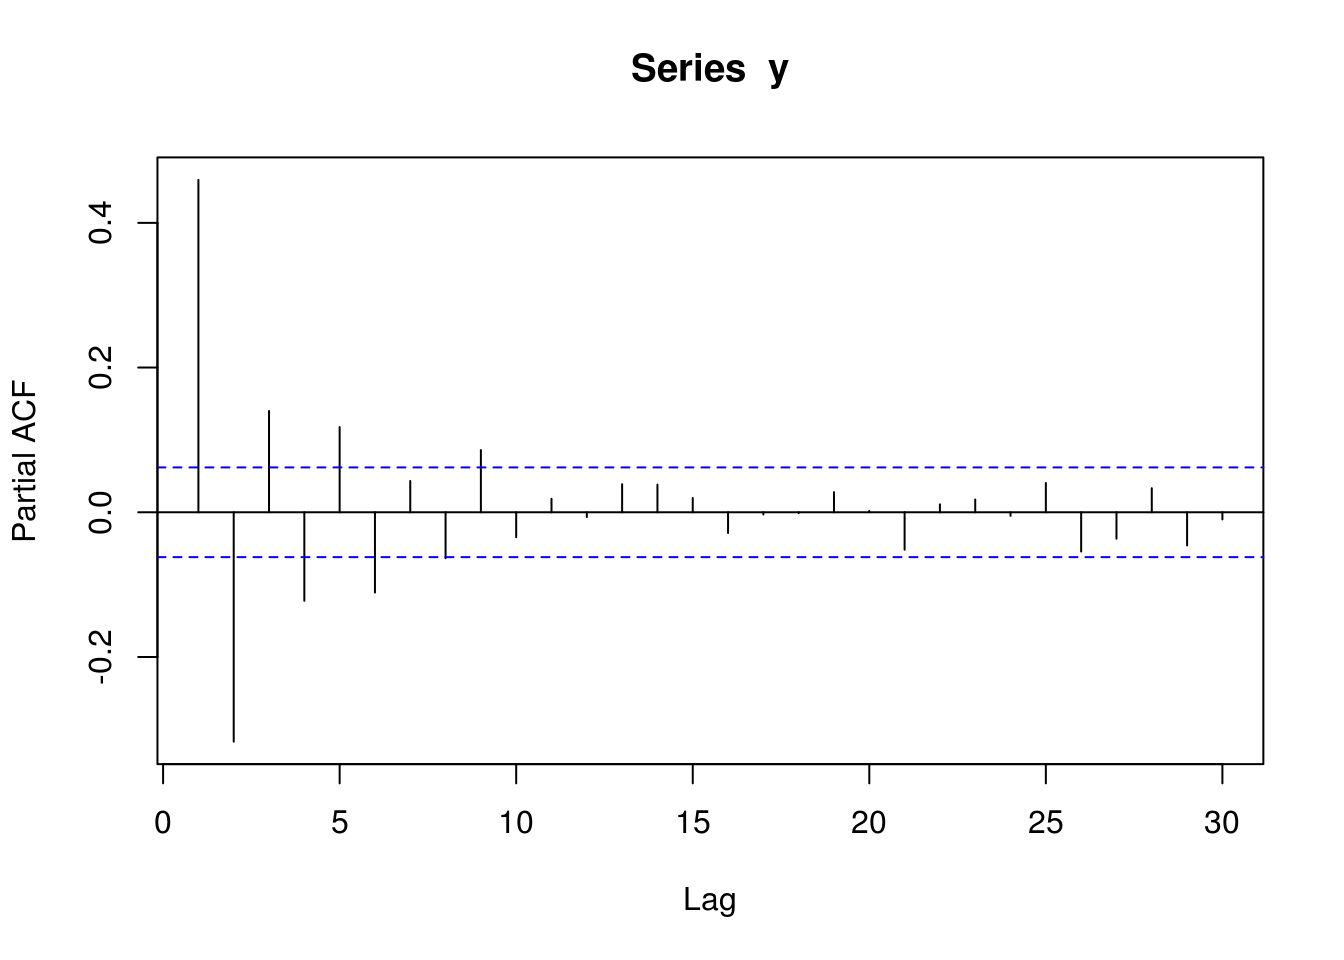
\includegraphics{website_files/figure-latex/unnamed-chunk-13-1.pdf}

\newpage

With \texttt{moving\ average} data, an \texttt{acf} plot contains a
number of sharp significant lines, demarking how many subsequent
observations have autocorrelation. i.e.~if one line is significant, it
means that each observation is only correlated with its preceeding
observation. If two lines are significant, it means that each
observation is correlated with its two preceeding observations. The
following plot represents \texttt{MA(1)} data. Note that the
\texttt{acf} plot displays \texttt{lag\ 0} (which is pointless and can
be ignored), while the \texttt{pacf} plot does not.

\begin{Shaded}
\begin{Highlighting}[]
\KeywordTok{acf}\NormalTok{(y)}
\end{Highlighting}
\end{Shaded}

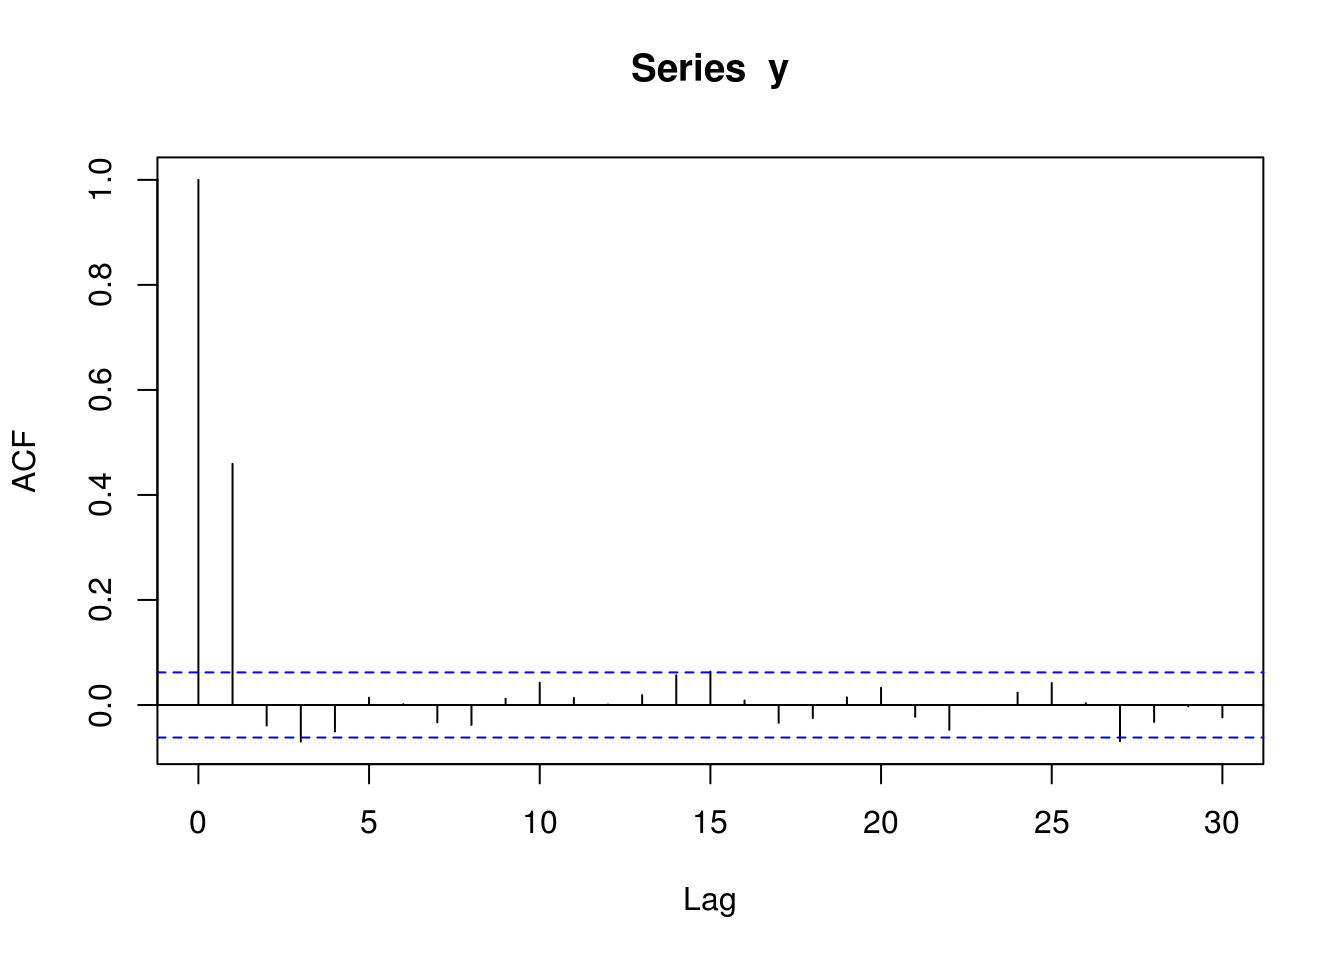
\includegraphics{website_files/figure-latex/unnamed-chunk-14-1.pdf}

\newpage 

\subsection{MA(2) data}\label{ma2-data}

\begin{Shaded}
\begin{Highlighting}[]
\NormalTok{y <-}\StringTok{ }\KeywordTok{round}\NormalTok{(}\KeywordTok{as.numeric}\NormalTok{(}\KeywordTok{arima.sim}\NormalTok{(}\DataTypeTok{model=}\KeywordTok{list}\NormalTok{(}\StringTok{"ma"}\NormalTok{=}\KeywordTok{c}\NormalTok{(}\FloatTok{0.9}\NormalTok{,}\FloatTok{0.6}\NormalTok{)), }\DataTypeTok{rand.gen =}\NormalTok{ rnorm, }\DataTypeTok{n=}\DecValTok{1000}\NormalTok{)))}
\end{Highlighting}
\end{Shaded}

The following \texttt{pacf} plot represents some sort of \texttt{MA}
data.

\begin{Shaded}
\begin{Highlighting}[]
\KeywordTok{pacf}\NormalTok{(y)}
\end{Highlighting}
\end{Shaded}

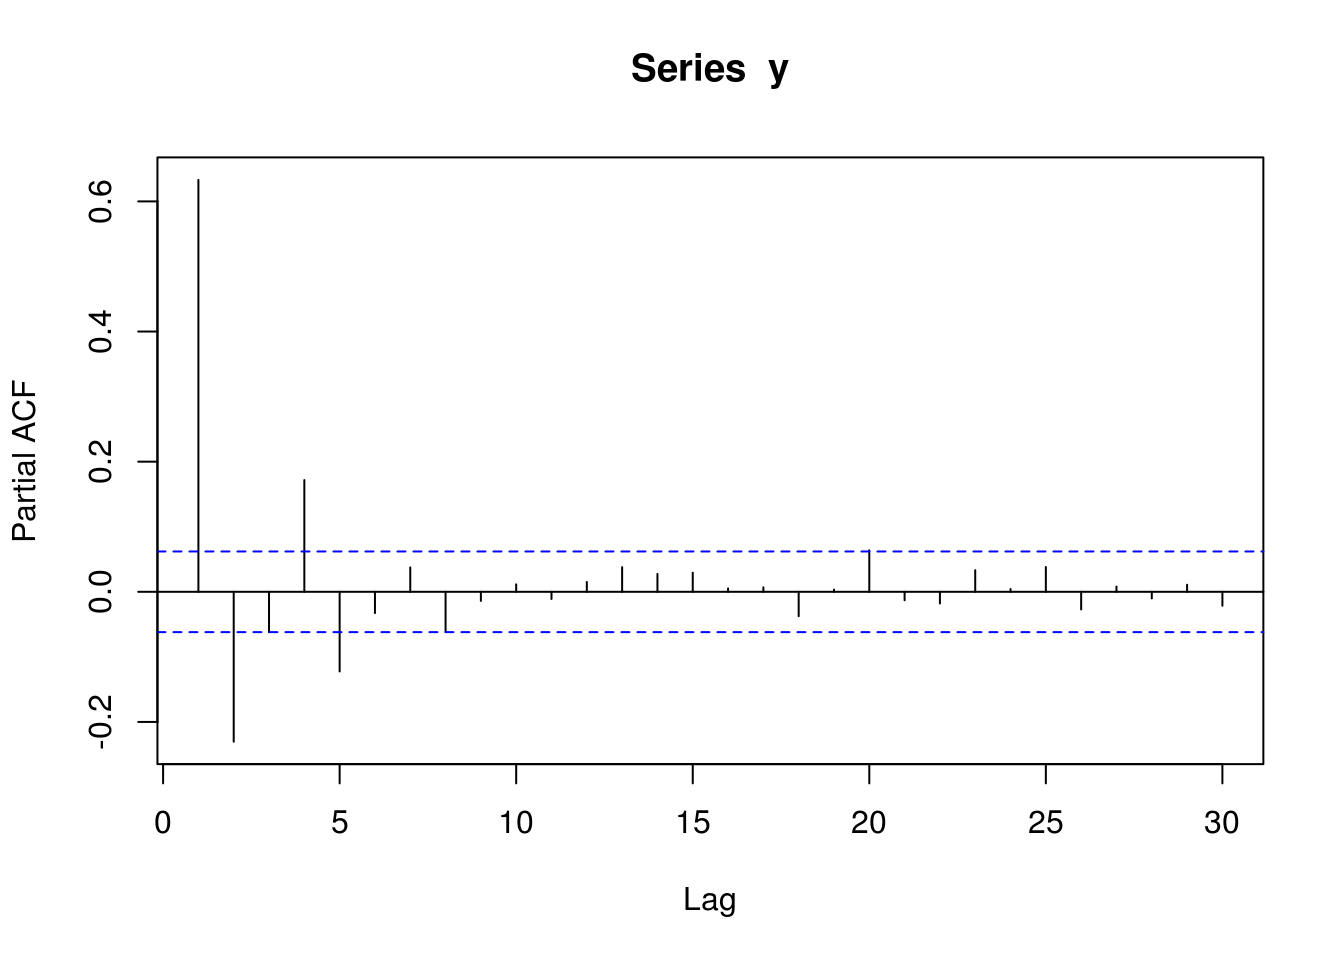
\includegraphics{website_files/figure-latex/unnamed-chunk-16-1.pdf}

\newpage

The following \texttt{acf} plot represents \texttt{MA(2)} data. This
means that each observation is correlated with its two preceeding
observations.

\begin{Shaded}
\begin{Highlighting}[]
\KeywordTok{acf}\NormalTok{(y)}
\end{Highlighting}
\end{Shaded}

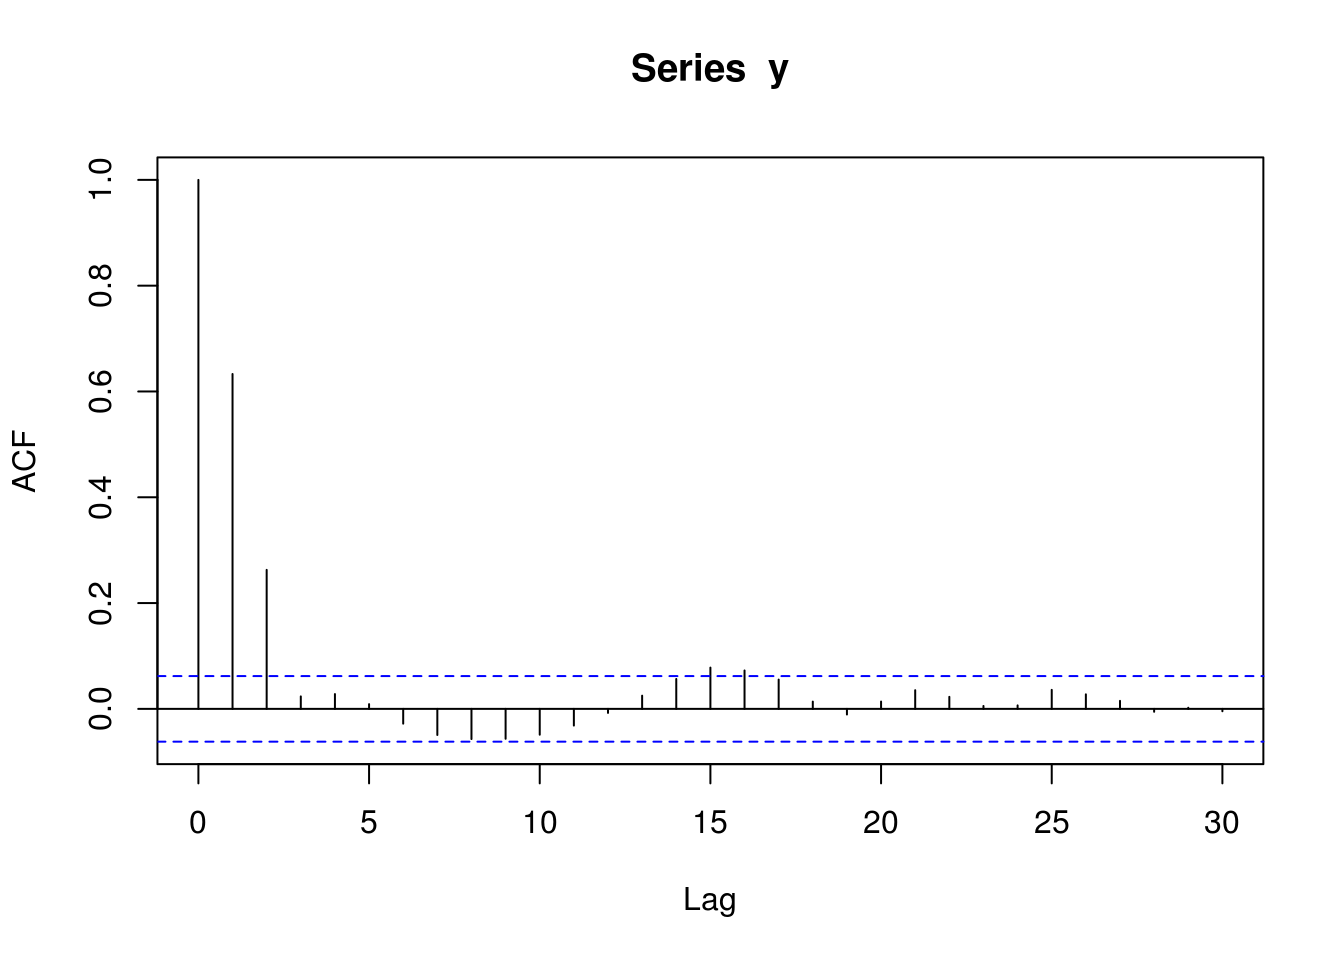
\includegraphics{website_files/figure-latex/unnamed-chunk-17-1.pdf}

\chapter{Panel data: One area without
autocorrelation}\label{panel-data-one-area-without-autocorrelation}

\section{Aim}\label{aim}

We are given a dataset containing daily counts of diseases from one
geographical area. We want to identify:

\begin{itemize}
\tightlist
\item
  Does seasonality exist?
\item
  If seasonality exists, when are the high/low seasons?
\item
  Is there a general yearly trend (i.e.~increasing or decreasing from
  year to year?)
\item
  Is daily rainfall associated with the number of cases?
\end{itemize}

\newpage

\section{Creating the data}\label{creating-the-data}

The data for this chapter is available at:
\url{http://rwhite.no/longitudinal_analysis/data/chapter_3.csv}

\begin{Shaded}
\begin{Highlighting}[]
\CommentTok{# R CODE}

\KeywordTok{dir.create}\NormalTok{(}\StringTok{"data"}\NormalTok{)}

\KeywordTok{library}\NormalTok{(data.table)}
\KeywordTok{library}\NormalTok{(ggplot2)}
\KeywordTok{set.seed}\NormalTok{(}\DecValTok{4}\NormalTok{)}

\NormalTok{AMPLITUDE <-}\StringTok{ }\FloatTok{1.5}
\NormalTok{SEASONAL_HORIZONTAL_SHIFT <-}\StringTok{ }\DecValTok{20}

\NormalTok{d <-}\StringTok{ }\KeywordTok{data.table}\NormalTok{(}\DataTypeTok{date=}\KeywordTok{seq.Date}\NormalTok{(}
  \DataTypeTok{from=}\KeywordTok{as.Date}\NormalTok{(}\StringTok{"2000-01-01"}\NormalTok{),}
  \DataTypeTok{to=}\KeywordTok{as.Date}\NormalTok{(}\StringTok{"2018-12-31"}\NormalTok{),}
  \DataTypeTok{by=}\DecValTok{1}\NormalTok{))}
\NormalTok{d[,year}\OperatorTok{:}\ErrorTok{=}\KeywordTok{as.numeric}\NormalTok{(}\KeywordTok{format.Date}\NormalTok{(date,}\StringTok{"%G"}\NormalTok{))]}
\NormalTok{d[,week}\OperatorTok{:}\ErrorTok{=}\KeywordTok{as.numeric}\NormalTok{(}\KeywordTok{format.Date}\NormalTok{(date,}\StringTok{"%V"}\NormalTok{))]}
\NormalTok{d[,month}\OperatorTok{:}\ErrorTok{=}\KeywordTok{as.numeric}\NormalTok{(}\KeywordTok{format.Date}\NormalTok{(date,}\StringTok{"%m"}\NormalTok{))]}
\NormalTok{d[,yearMinus2000}\OperatorTok{:}\ErrorTok{=}\NormalTok{year}\OperatorTok{-}\DecValTok{2000}\NormalTok{]}
\NormalTok{d[,dailyrainfall}\OperatorTok{:}\ErrorTok{=}\KeywordTok{runif}\NormalTok{(.N, }\DataTypeTok{min=}\DecValTok{0}\NormalTok{, }\DataTypeTok{max=}\DecValTok{10}\NormalTok{)]}

\NormalTok{d[,dayOfYear}\OperatorTok{:}\ErrorTok{=}\KeywordTok{as.numeric}\NormalTok{(}\KeywordTok{format.Date}\NormalTok{(date,}\StringTok{"%j"}\NormalTok{))]}
\NormalTok{d[,seasonalEffect}\OperatorTok{:}\ErrorTok{=}\KeywordTok{sin}\NormalTok{(}\DecValTok{2}\OperatorTok{*}\NormalTok{pi}\OperatorTok{*}\NormalTok{(dayOfYear}\OperatorTok{-}\NormalTok{SEASONAL_HORIZONTAL_SHIFT)}\OperatorTok{/}\DecValTok{365}\NormalTok{)]}
\NormalTok{d[,mu }\OperatorTok{:}\ErrorTok{=}\StringTok{ }\KeywordTok{exp}\NormalTok{(}\FloatTok{0.1} \OperatorTok{+}\StringTok{ }\NormalTok{yearMinus2000}\OperatorTok{*}\FloatTok{0.1} \OperatorTok{+}\StringTok{ }\NormalTok{seasonalEffect}\OperatorTok{*}\NormalTok{AMPLITUDE)]}
\NormalTok{d[,y}\OperatorTok{:}\ErrorTok{=}\KeywordTok{rpois}\NormalTok{(.N,mu)]}

\KeywordTok{fwrite}\NormalTok{(d,}\StringTok{"data/chapter_3.csv"}\NormalTok{)}
\end{Highlighting}
\end{Shaded}

\newpage

\section{True data}\label{true-data}

Here we show the true data, and note that there is an increasing annual
trend (the data gets higher as time goes on) and there is a seasonal
pattern (one peak/trough per year)

\begin{Shaded}
\begin{Highlighting}[]
\NormalTok{q <-}\StringTok{ }\KeywordTok{ggplot}\NormalTok{(d,}\KeywordTok{aes}\NormalTok{(}\DataTypeTok{x=}\NormalTok{date))}
\NormalTok{q <-}\StringTok{ }\NormalTok{q }\OperatorTok{+}\StringTok{ }\KeywordTok{geom_point}\NormalTok{(}\DataTypeTok{mapping=}\KeywordTok{aes}\NormalTok{(}\DataTypeTok{y=}\NormalTok{y))}
\NormalTok{q <-}\StringTok{ }\NormalTok{q }\OperatorTok{+}\StringTok{ }\KeywordTok{geom_line}\NormalTok{(}\DataTypeTok{mapping=}\KeywordTok{aes}\NormalTok{(}\DataTypeTok{y=}\NormalTok{mu),}\DataTypeTok{colour=}\StringTok{"red"}\NormalTok{)}
\NormalTok{q}
\end{Highlighting}
\end{Shaded}

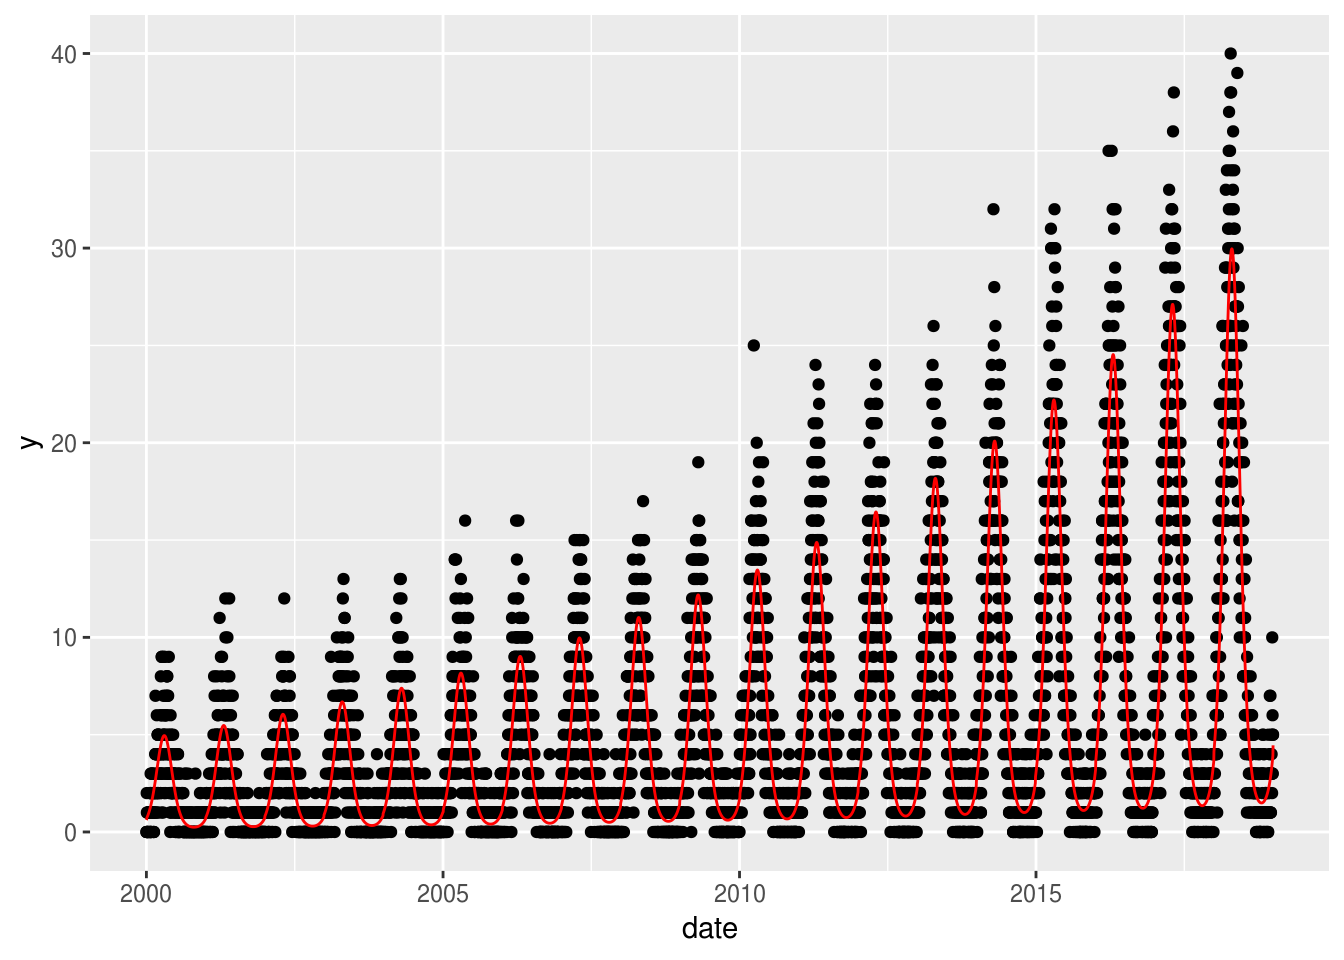
\includegraphics{website_files/figure-latex/unnamed-chunk-19-1.pdf}

\newpage

\section{Investigation}\label{investigation}

Pretending we have no prior knowledge of our dataset, we display the
data for few years and see a clear seasonal trend

\begin{Shaded}
\begin{Highlighting}[]
\NormalTok{q <-}\StringTok{ }\KeywordTok{ggplot}\NormalTok{(d[year }\OperatorTok\StringTok{ }\KeywordTok{c}\NormalTok{(}\DecValTok{2005}\OperatorTok{:}\DecValTok{2010}\NormalTok{)],}\KeywordTok{aes}\NormalTok{(}\DataTypeTok{x=}\NormalTok{dayOfYear,}\DataTypeTok{y=}\NormalTok{y))}
\NormalTok{q <-}\StringTok{ }\NormalTok{q }\OperatorTok{+}\StringTok{ }\KeywordTok{facet_wrap}\NormalTok{(}\OperatorTok{~}\NormalTok{year)}
\NormalTok{q <-}\StringTok{ }\NormalTok{q }\OperatorTok{+}\StringTok{ }\KeywordTok{geom_point}\NormalTok{()}
\NormalTok{q <-}\StringTok{ }\NormalTok{q }\OperatorTok{+}\StringTok{ }\KeywordTok{stat_smooth}\NormalTok{(}\DataTypeTok{colour=}\StringTok{"red"}\NormalTok{)}
\NormalTok{q}
\end{Highlighting}
\end{Shaded}

\begin{verbatim}
## `geom_smooth()` using method = 'loess' and formula 'y ~ x'
\end{verbatim}

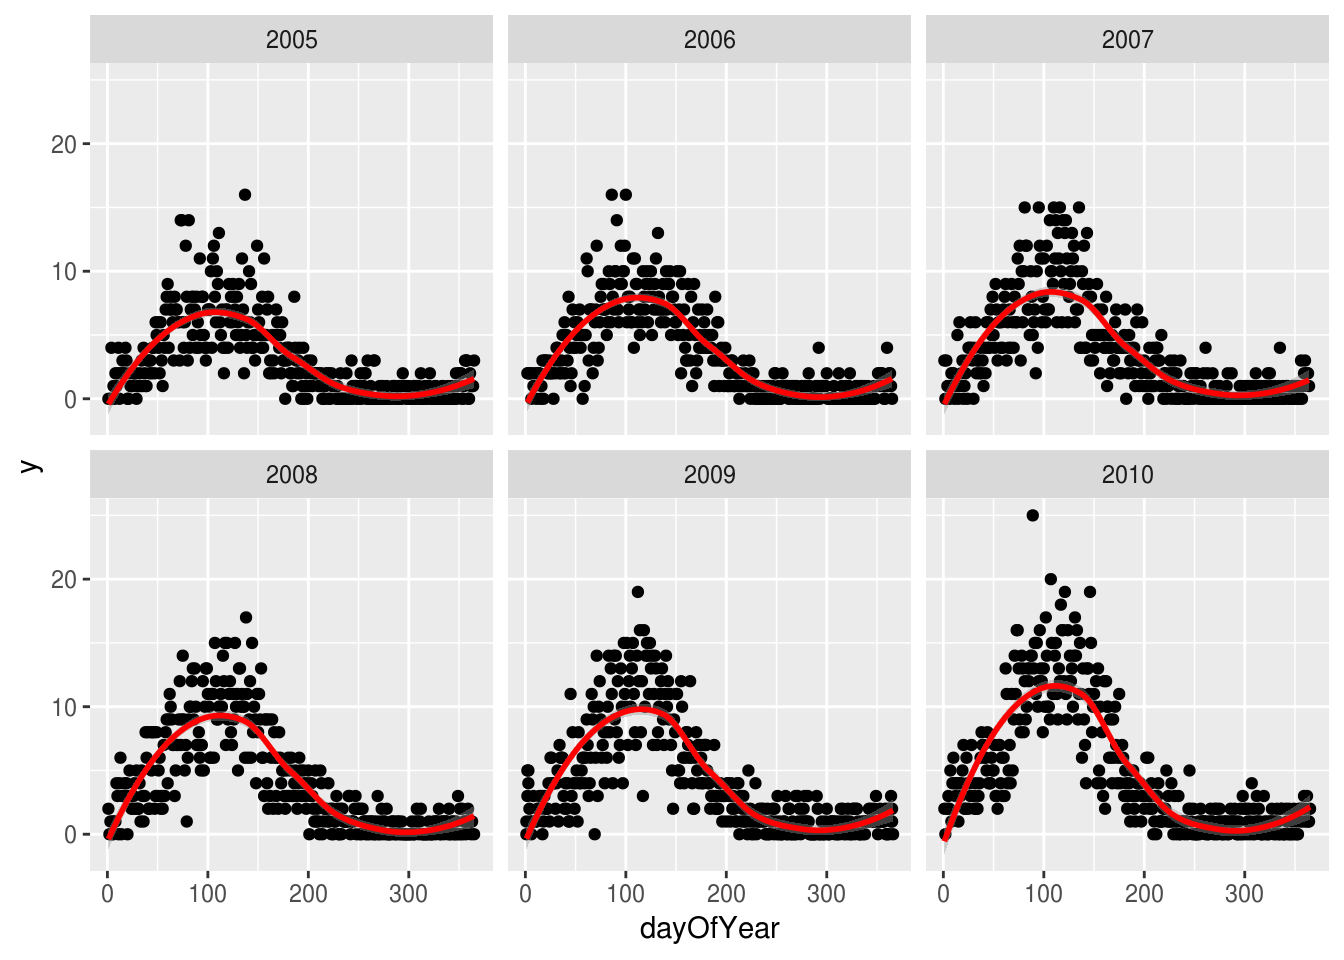
\includegraphics{website_files/figure-latex/unnamed-chunk-20-1.pdf}

\newpage

\section{Seasonality}\label{seasonality}

If we want to investigate the seasonality of our data, and identify when
are the peaks and troughs, we have a few ways to approach this.

Non-parametric approaches are flexible and easy to implement, but they
can lack power and be hard to interpret:

\begin{itemize}
\tightlist
\item
  Create a categorical variable for the seasons (e.g. \texttt{spring},
  \texttt{summer}, \texttt{autumn}, \texttt{winter}) and include this in
  the regression model
\item
  Create a categorical variable for the months (e.g. \texttt{Jan},
  \texttt{Feb}, \ldots{}, \texttt{Dec}) and include this in the
  regression model
\end{itemize}

Parametric approaches are more powerful but require more effort:

\begin{itemize}
\tightlist
\item
  Identify the periodicity of the seasonality (how many days between
  peaks?)
\item
  Using trigonometry, transform \texttt{day\ of\ year} into variables
  that appropriately model the observed periodicity
\item
  Obtain coefficient estimates
\item
  Back-transform these estimates into human-understandable values (day
  of peak, day of trough)
\end{itemize}

The non-parametric approaches are simple and we will therefore not cover
them in this course. We will briefly examine the parametric approach.

\emph{NOTE:} You don't always have to investigate seasonality! It
depends entirely on what the purpose of your analysis is!

\newpage

The Lomb-Scargle Periodogram shows a clear seasonality with a period of
365 days.

\begin{verbatim}
// STATA CODE STARTS
insheet using "chapter_3.csv", clear

sort date
gen time=_n
tsset time, daily

wntestb y

cumsp y, gen(cumulative_spec_dist)
gen period=_N/_n

browse cumulative_spec_dist period
// STATA CODE ENDS
\end{verbatim}

\begin{Shaded}
\begin{Highlighting}[]
\CommentTok{# R CODE }
\NormalTok{lomb}\OperatorTok{::}\KeywordTok{lsp}\NormalTok{(d}\OperatorTok{$}\NormalTok{y,}\DataTypeTok{from=}\DecValTok{100}\NormalTok{,}\DataTypeTok{to=}\DecValTok{500}\NormalTok{,}\DataTypeTok{ofac=}\DecValTok{1}\NormalTok{,}\DataTypeTok{type=}\StringTok{"period"}\NormalTok{)}
\end{Highlighting}
\end{Shaded}

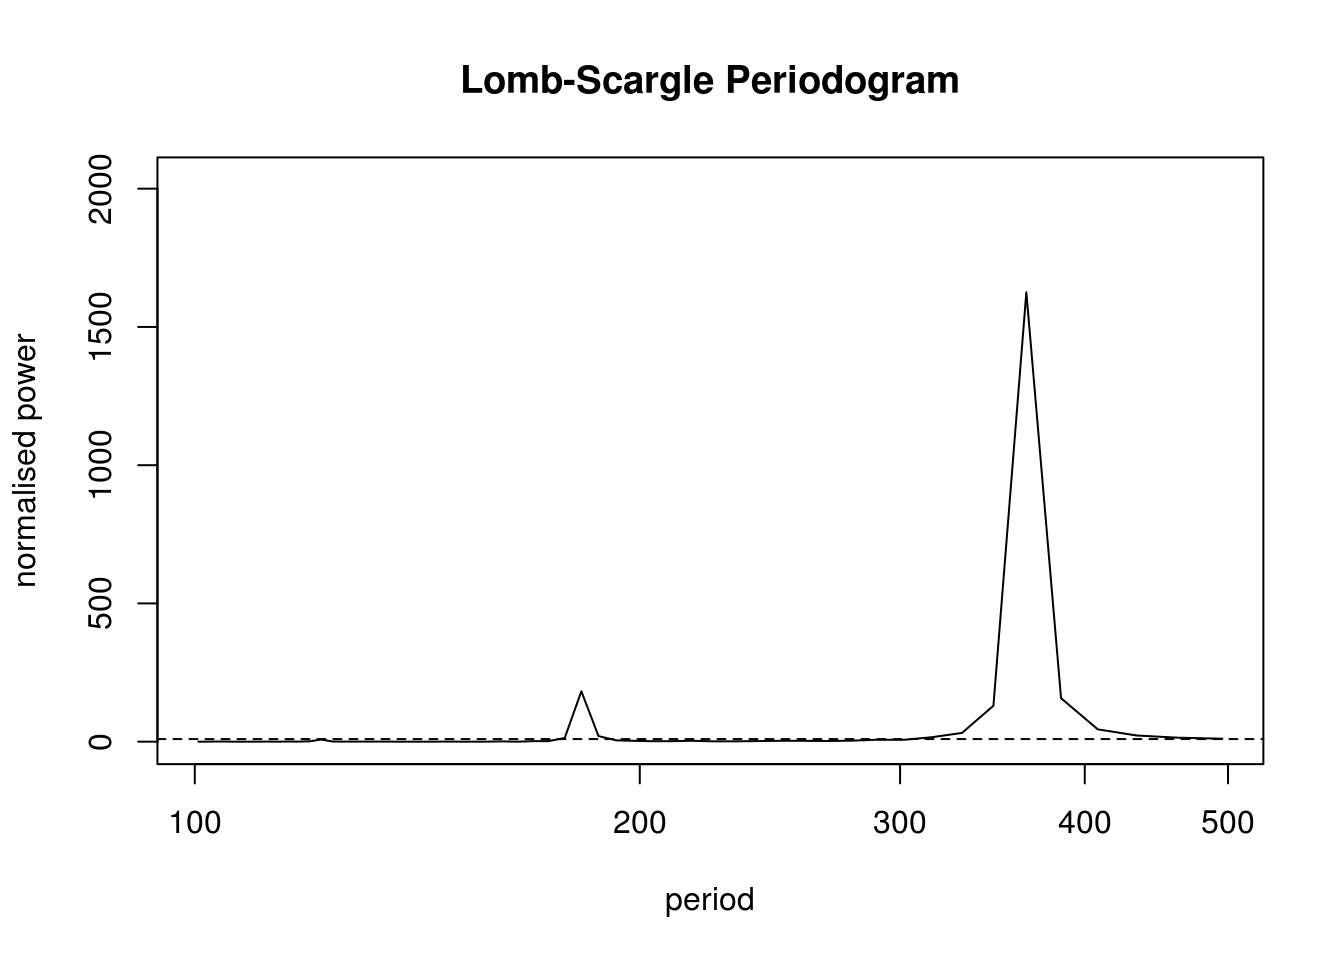
\includegraphics{website_files/figure-latex/unnamed-chunk-21-1.pdf}

\newpage

We then generate two new variables \texttt{cos365} and \texttt{sin365}
and perform a likelihood ratio test to see if they are significant or
not. This is done with two simple poisson regressions.

When we do not have autocorrelation, we can use the \texttt{glm}
function in R and in STATA. Note that it is very important to specify
the \texttt{family} (as this is how we differentiate between
linear/logistic/poisson regressions).

\begin{verbatim}
// STATA CODE STARTS
gen cos365=cos(dayofyear*2*_pi/365)
gen sin365=sin(dayofyear*2*_pi/365)

glm y yearminus2000 dailyrainfall, family(poisson)
estimates store m1
glm y yearminus2000 dailyrainfall cos365 sin365, family(poisson)
estimates store m2

predict resid, anscombe

lrtest m1 m2
// STATA CODE ENDS
\end{verbatim}

\begin{Shaded}
\begin{Highlighting}[]
\CommentTok{# R CODE}
\NormalTok{d[,cos365}\OperatorTok{:}\ErrorTok{=}\KeywordTok{cos}\NormalTok{(dayOfYear}\OperatorTok{*}\DecValTok{2}\OperatorTok{*}\NormalTok{pi}\OperatorTok{/}\DecValTok{365}\NormalTok{)]}
\NormalTok{d[,sin365}\OperatorTok{:}\ErrorTok{=}\KeywordTok{sin}\NormalTok{(dayOfYear}\OperatorTok{*}\DecValTok{2}\OperatorTok{*}\NormalTok{pi}\OperatorTok{/}\DecValTok{365}\NormalTok{)]}

\NormalTok{fit0 <-}\StringTok{ }\KeywordTok{glm}\NormalTok{(y}\OperatorTok{~}\NormalTok{yearMinus2000 }\OperatorTok{+}\StringTok{ }\NormalTok{dailyrainfall, }\DataTypeTok{data=}\NormalTok{d, }\DataTypeTok{family=}\KeywordTok{poisson}\NormalTok{())}
\NormalTok{fit1 <-}\StringTok{ }\KeywordTok{glm}\NormalTok{(y}\OperatorTok{~}\NormalTok{yearMinus2000 }\OperatorTok{+}\StringTok{ }\NormalTok{dailyrainfall }\OperatorTok{+}\StringTok{ }\NormalTok{sin365 }\OperatorTok{+}\StringTok{ }\NormalTok{cos365, }\DataTypeTok{data=}\NormalTok{d, }\DataTypeTok{family=}\KeywordTok{poisson}\NormalTok{())}

\KeywordTok{print}\NormalTok{(lmtest}\OperatorTok{::}\KeywordTok{lrtest}\NormalTok{(fit0, fit1))}
\end{Highlighting}
\end{Shaded}

\begin{verbatim}
## Likelihood ratio test
## 
## Model 1: y ~ yearMinus2000 + dailyrainfall
## Model 2: y ~ yearMinus2000 + dailyrainfall + sin365 + cos365
##   #Df LogLik Df Chisq Pr(>Chisq)    
## 1   3 -26904                        
## 2   5 -12892  2 28024  < 2.2e-16 ***
## ---
## Signif. codes:  0 '***' 0.001 '**' 0.01 '*' 0.05 '.' 0.1 ' ' 1
\end{verbatim}

We see that the likelihood ratio test for \texttt{sin365} and
\texttt{cos365} was significant, meaning that there is significant
seasonality with a 365 day periodicity in our data (which we already
strongly suspected due to the periodogram).

\newpage

We can now run/look at the results of our main regression.

\begin{Shaded}
\begin{Highlighting}[]
\KeywordTok{print}\NormalTok{(}\KeywordTok{summary}\NormalTok{(fit1))}
\end{Highlighting}
\end{Shaded}

\begin{verbatim}
## 
## Call:
## glm(formula = y ~ yearMinus2000 + dailyrainfall + sin365 + cos365, 
##     family = poisson(), data = d)
## 
## Deviance Residuals: 
##     Min       1Q   Median       3Q      Max  
## -4.0676  -0.9229  -0.1170   0.5861   3.4103  
## 
## Coefficients:
##                 Estimate Std. Error z value Pr(>|z|)    
## (Intercept)    0.0887436  0.0176742   5.021 5.14e-07 ***
## yearMinus2000  0.1016117  0.0010525  96.539  < 2e-16 ***
## dailyrainfall  0.0002287  0.0018476   0.124    0.901    
## sin365         1.3972586  0.0103200 135.393  < 2e-16 ***
## cos365        -0.5035265  0.0086308 -58.341  < 2e-16 ***
## ---
## Signif. codes:  0 '***' 0.001 '**' 0.01 '*' 0.05 '.' 0.1 ' ' 1
## 
## (Dispersion parameter for poisson family taken to be 1)
## 
##     Null deviance: 45536.8  on 6939  degrees of freedom
## Residual deviance:  7328.5  on 6935  degrees of freedom
## AIC: 25794
## 
## Number of Fisher Scoring iterations: 5
\end{verbatim}

We also see that the (significant!) coefficient for \texttt{year} is
\texttt{0.1} which means that for each additional year, the outcome
increases by \texttt{exp(0.1)=1.11}. We also see that the coefficient
for \texttt{dailyrainfall} was not significant, which means that we did
not find a significant association between the outcome and
\texttt{dailyrainfall}.

\emph{NOTE:} See that this is basically the same as a normal regression.

\newpage

Through the likelihood ratio test we saw a clear significant seasonal
effect. We can now use trigonometry to back-calculate the amplitude and
location of peak/troughs from the \texttt{cos365} and \texttt{sin365}
estimates:

\begin{Shaded}
\begin{Highlighting}[]
\NormalTok{b1 <-}\StringTok{ }\FloatTok{1.428417} \CommentTok{# sin coefficient}
\NormalTok{b2 <-}\StringTok{ }\OperatorTok{-}\FloatTok{0.512912} \CommentTok{# cos coefficient}
\NormalTok{amplitude <-}\StringTok{ }\KeywordTok{sqrt}\NormalTok{(b1}\OperatorTok{^}\DecValTok{2} \OperatorTok{+}\StringTok{ }\NormalTok{b2}\OperatorTok{^}\DecValTok{2}\NormalTok{)}
\NormalTok{p <-}\StringTok{ }\KeywordTok{atan}\NormalTok{(b1}\OperatorTok{/}\NormalTok{b2) }\OperatorTok{*}\StringTok{ }\DecValTok{365}\OperatorTok{/}\DecValTok{2}\OperatorTok{/}\NormalTok{pi}
\ControlFlowTok{if}\NormalTok{ (p }\OperatorTok{>}\StringTok{ }\DecValTok{0}\NormalTok{) \{}
\NormalTok{    peak <-}\StringTok{ }\NormalTok{p}
\NormalTok{    trough <-}\StringTok{ }\NormalTok{p }\OperatorTok{+}\StringTok{ }\DecValTok{365}\OperatorTok{/}\DecValTok{2}
\NormalTok{\} }\ControlFlowTok{else}\NormalTok{ \{}
\NormalTok{    peak <-}\StringTok{ }\NormalTok{p }\OperatorTok{+}\StringTok{ }\DecValTok{365}\OperatorTok{/}\DecValTok{2}
\NormalTok{    trough <-}\StringTok{ }\NormalTok{p }\OperatorTok{+}\StringTok{ }\DecValTok{365}
\NormalTok{\}}
\ControlFlowTok{if}\NormalTok{ (b1 }\OperatorTok{<}\StringTok{ }\DecValTok{0}\NormalTok{) \{}
\NormalTok{    g <-}\StringTok{ }\NormalTok{peak}
\NormalTok{    peak <-}\StringTok{ }\NormalTok{trough}
\NormalTok{    trough <-}\StringTok{ }\NormalTok{g}
\NormalTok{\}}
\KeywordTok{print}\NormalTok{(}\KeywordTok{sprintf}\NormalTok{(}\StringTok{"amplitude is estimated as %s, peak is estimated as %s, trough is estimated as %s"}\NormalTok{,}\KeywordTok{round}\NormalTok{(amplitude,}\DecValTok{2}\NormalTok{),}\KeywordTok{round}\NormalTok{(peak),}\KeywordTok{round}\NormalTok{(trough)))}
\end{Highlighting}
\end{Shaded}

\begin{verbatim}
## [1] "amplitude is estimated as 1.52, peak is estimated as 111, trough is estimated as 294"
\end{verbatim}

\begin{Shaded}
\begin{Highlighting}[]
\KeywordTok{print}\NormalTok{(}\KeywordTok{sprintf}\NormalTok{(}\StringTok{"true values are: amplitude: %s, peak: %s, trough: %s"}\NormalTok{,}\KeywordTok{round}\NormalTok{(AMPLITUDE,}\DecValTok{2}\NormalTok{),}\KeywordTok{round}\NormalTok{(}\DecValTok{365}\OperatorTok{/}\DecValTok{4}\OperatorTok{+}\NormalTok{SEASONAL_HORIZONTAL_SHIFT),}\KeywordTok{round}\NormalTok{(}\DecValTok{3}\OperatorTok{*}\DecValTok{365}\OperatorTok{/}\DecValTok{4}\OperatorTok{+}\NormalTok{SEASONAL_HORIZONTAL_SHIFT)))}
\end{Highlighting}
\end{Shaded}

\begin{verbatim}
## [1] "true values are: amplitude: 1.5, peak: 111, trough: 294"
\end{verbatim}

\emph{NOTE:} An amplitude of 1.5 means that when comparing the average
time of year to the peak, the peak is expected to be
\texttt{exp(1.5)=4.5} times higher than average. We take the exponential
because we have run a poisson regression (so think incident rate ratio).

\newpage

We now investigate our residuals to determine if we have a good fit:

\begin{Shaded}
\begin{Highlighting}[]
\NormalTok{d[,residuals}\OperatorTok{:}\ErrorTok{=}\KeywordTok{residuals}\NormalTok{(fit1, }\DataTypeTok{type =} \StringTok{"response"}\NormalTok{)]}
\NormalTok{d[,predicted}\OperatorTok{:}\ErrorTok{=}\KeywordTok{predict}\NormalTok{(fit1, }\DataTypeTok{type =} \StringTok{"response"}\NormalTok{)]}
\NormalTok{q <-}\StringTok{ }\KeywordTok{ggplot}\NormalTok{(d,}\KeywordTok{aes}\NormalTok{(}\DataTypeTok{x=}\NormalTok{predicted,}\DataTypeTok{y=}\NormalTok{residuals))}
\NormalTok{q <-}\StringTok{ }\NormalTok{q }\OperatorTok{+}\StringTok{ }\KeywordTok{geom_point}\NormalTok{()}
\NormalTok{q <-}\StringTok{ }\NormalTok{q }\OperatorTok{+}\StringTok{ }\KeywordTok{stat_smooth}\NormalTok{(}\DataTypeTok{colour=}\StringTok{"red"}\NormalTok{)}
\NormalTok{q}
\end{Highlighting}
\end{Shaded}

\begin{verbatim}
## `geom_smooth()` using method = 'gam' and formula 'y ~ s(x, bs = "cs")'
\end{verbatim}

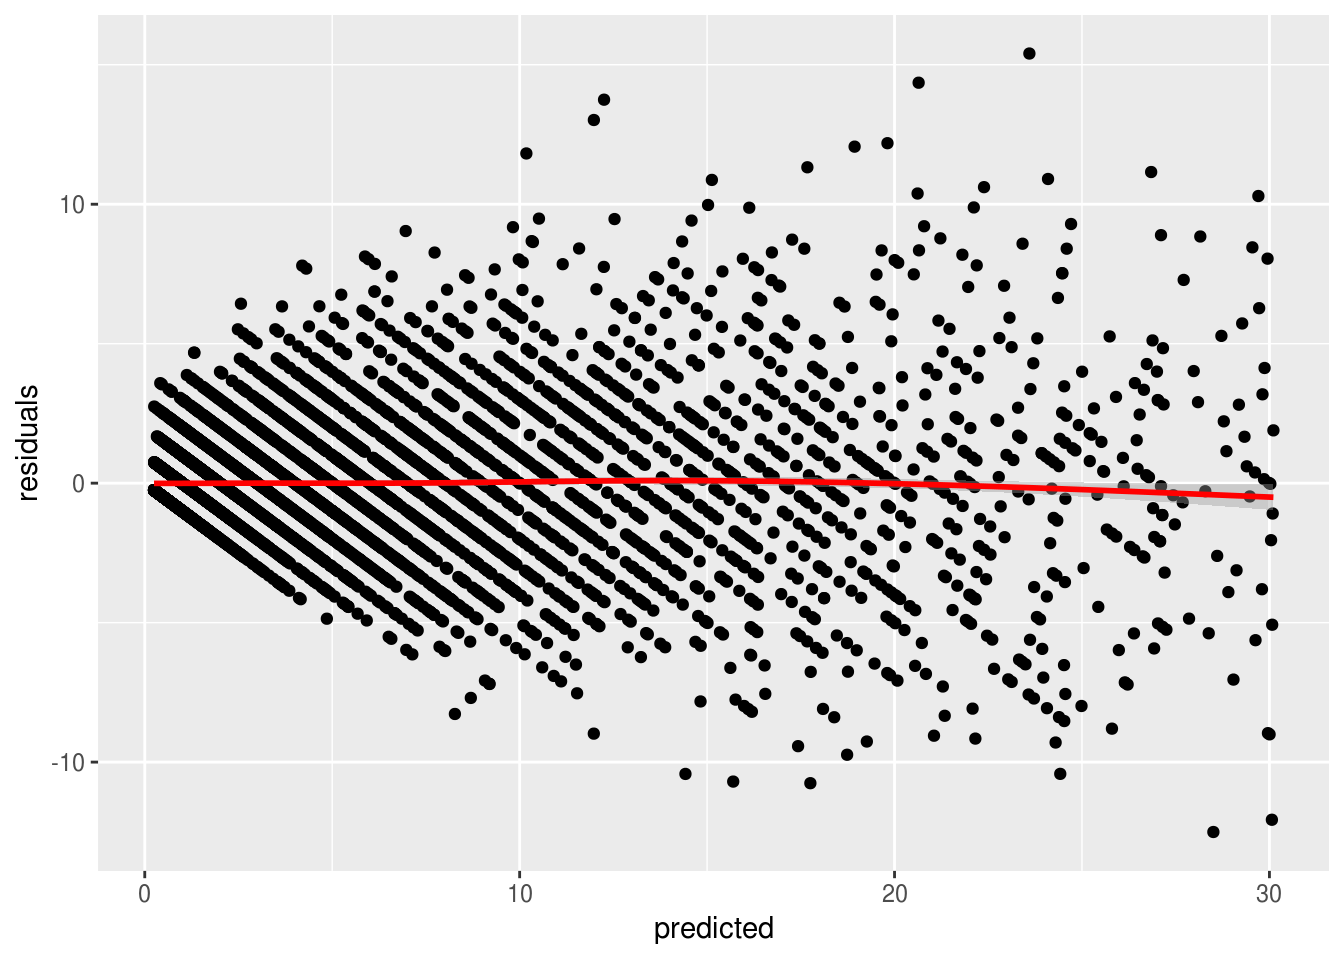
\includegraphics{website_files/figure-latex/unnamed-chunk-25-1.pdf}

\newpage

We check the \texttt{pacf} of the residuals to ensure that it is not
\texttt{AR}. If we observe \texttt{AR} in our residuals, then this model
was not appropriate and we need to use a different model.

\begin{verbatim}
// STATA CODE STARTS
pac resid
// STATA CODE ENDS
\end{verbatim}

\begin{Shaded}
\begin{Highlighting}[]
\CommentTok{# R CODE}
\CommentTok{# this is for AR}
\KeywordTok{pacf}\NormalTok{(d}\OperatorTok{$}\NormalTok{residuals)}
\end{Highlighting}
\end{Shaded}

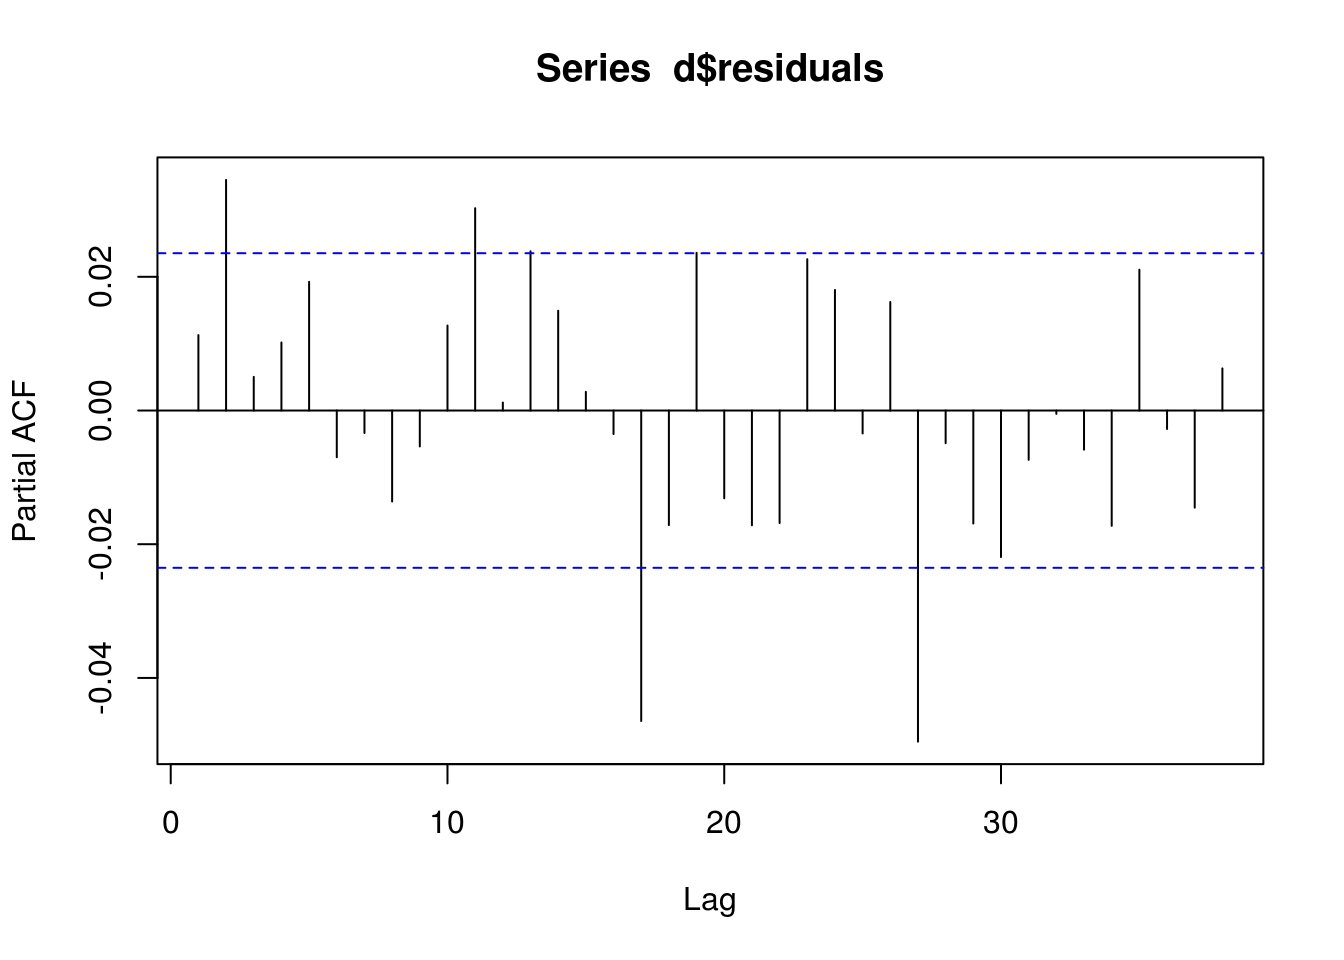
\includegraphics{website_files/figure-latex/unnamed-chunk-26-1.pdf}

\newpage

We check the \texttt{acf} of the residuals to ensure that it is not
\texttt{MA}. If we observe \texttt{MA} in our residuals, then this model
was not appropriate and we need to use a different model.

\begin{verbatim}
// STATA CODE STARTS
ac resid
// STATA CODE ENDS
\end{verbatim}

\begin{Shaded}
\begin{Highlighting}[]
\CommentTok{# R CODE}
\CommentTok{# this is for MA}
\KeywordTok{acf}\NormalTok{(d}\OperatorTok{$}\NormalTok{residuals)}
\end{Highlighting}
\end{Shaded}

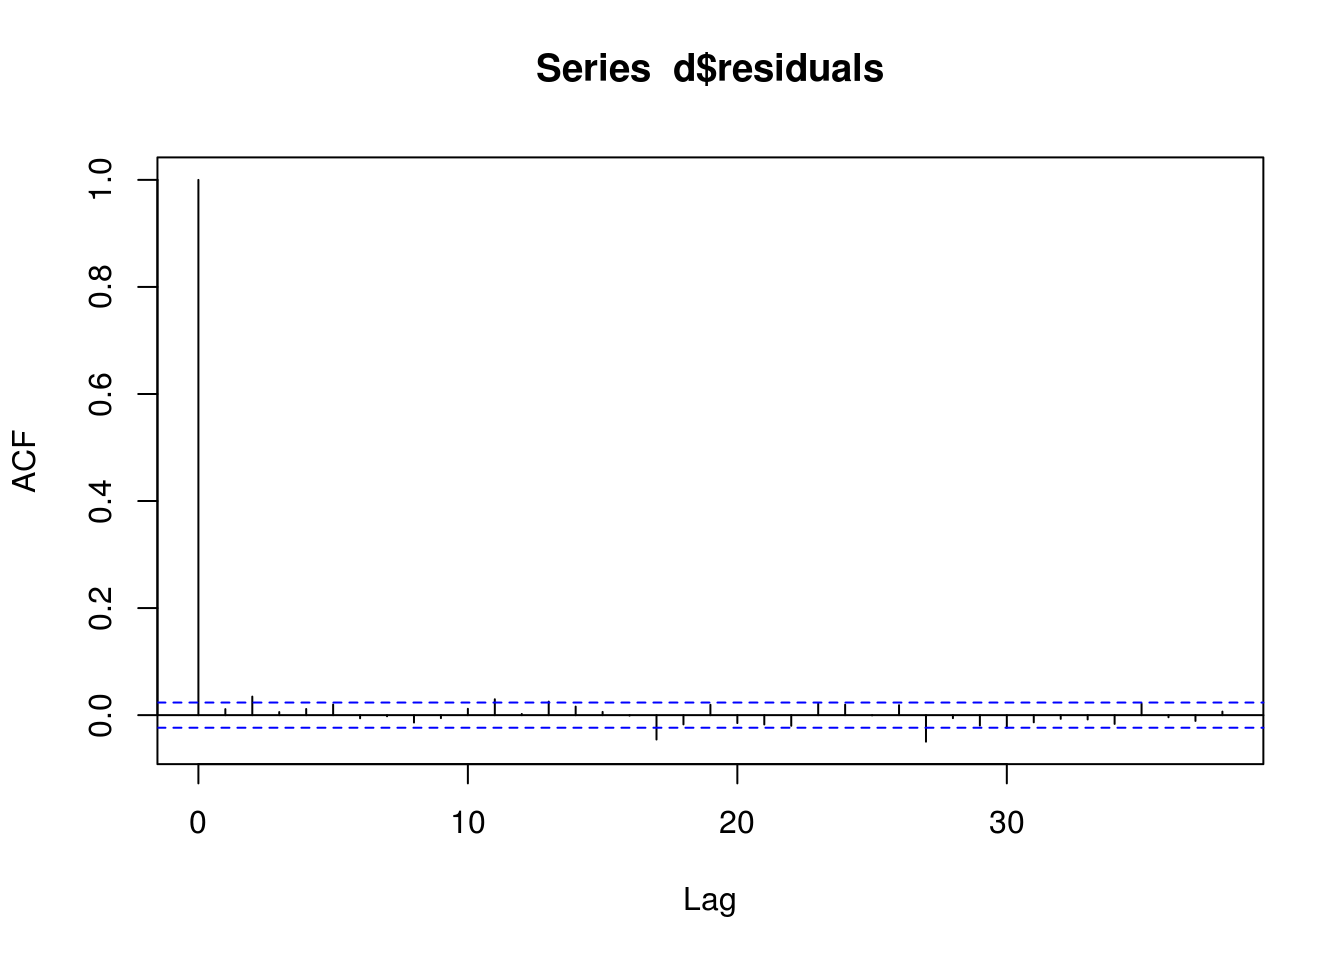
\includegraphics{website_files/figure-latex/unnamed-chunk-27-1.pdf}

\chapter{Panel data: One area with
autocorrelation}\label{panel-data-one-area-with-autocorrelation}

\section{Aim}\label{aim-1}

We are given a dataset containing daily counts of diseases from one
geographical area. We want to identify:

\begin{itemize}
\tightlist
\item
  Does seasonality exist?
\item
  If seasonality exists, when are the high/low seasons?
\item
  Is there a general yearly trend (i.e.~increasing or decreasing from
  year to year?)
\end{itemize}

(We remove the question about rainfall in order to simplify and
streamline the exercise)

\newpage

\section{Creating the data}\label{creating-the-data-1}

The data for this chapter is available at:
\url{http://rwhite.no/longitudinal_analysis/data/chapter_4.csv}

\begin{Shaded}
\begin{Highlighting}[]
\KeywordTok{library}\NormalTok{(data.table)}
\KeywordTok{library}\NormalTok{(ggplot2)}
\KeywordTok{set.seed}\NormalTok{(}\DecValTok{4}\NormalTok{)}

\NormalTok{AMPLITUDE <-}\StringTok{ }\FloatTok{1.5}
\NormalTok{SEASONAL_HORIZONTAL_SHIFT <-}\StringTok{ }\DecValTok{20}

\NormalTok{d <-}\StringTok{ }\KeywordTok{data.table}\NormalTok{(}\DataTypeTok{date=}\KeywordTok{seq.Date}\NormalTok{(}
  \DataTypeTok{from=}\KeywordTok{as.Date}\NormalTok{(}\StringTok{"2000-01-01"}\NormalTok{),}
  \DataTypeTok{to=}\KeywordTok{as.Date}\NormalTok{(}\StringTok{"2018-12-31"}\NormalTok{),}
  \DataTypeTok{by=}\DecValTok{1}\NormalTok{))}
\NormalTok{d[,year}\OperatorTok{:}\ErrorTok{=}\KeywordTok{as.numeric}\NormalTok{(}\KeywordTok{format.Date}\NormalTok{(date,}\StringTok{"%G"}\NormalTok{))]}
\NormalTok{d[,week}\OperatorTok{:}\ErrorTok{=}\KeywordTok{as.numeric}\NormalTok{(}\KeywordTok{format.Date}\NormalTok{(date,}\StringTok{"%V"}\NormalTok{))]}
\NormalTok{d[,month}\OperatorTok{:}\ErrorTok{=}\KeywordTok{as.numeric}\NormalTok{(}\KeywordTok{format.Date}\NormalTok{(date,}\StringTok{"%m"}\NormalTok{))]}
\NormalTok{d[,yearMinus2000}\OperatorTok{:}\ErrorTok{=}\NormalTok{year}\OperatorTok{-}\DecValTok{2000}\NormalTok{]}
\NormalTok{d[,dayOfSeries}\OperatorTok{:}\ErrorTok{=}\DecValTok{1}\OperatorTok{:}\NormalTok{.N]}

\NormalTok{d[,dayOfYear}\OperatorTok{:}\ErrorTok{=}\KeywordTok{as.numeric}\NormalTok{(}\KeywordTok{format.Date}\NormalTok{(date,}\StringTok{"%j"}\NormalTok{))]}
\NormalTok{d[,seasonalEffect}\OperatorTok{:}\ErrorTok{=}\KeywordTok{sin}\NormalTok{(}\DecValTok{2}\OperatorTok{*}\NormalTok{pi}\OperatorTok{*}\NormalTok{(dayOfYear}\OperatorTok{-}\NormalTok{SEASONAL_HORIZONTAL_SHIFT)}\OperatorTok{/}\DecValTok{365}\NormalTok{)]}
\NormalTok{d[,mu }\OperatorTok{:}\ErrorTok{=}\StringTok{ }\KeywordTok{exp}\NormalTok{(}\FloatTok{0.1} \OperatorTok{+}\StringTok{ }\NormalTok{yearMinus2000}\OperatorTok{*}\FloatTok{0.1} \OperatorTok{+}\StringTok{ }\NormalTok{seasonalEffect}\OperatorTok{*}\NormalTok{AMPLITUDE)]}
\NormalTok{d[,y}\OperatorTok{:}\ErrorTok{=}\KeywordTok{rpois}\NormalTok{(.N,mu)]}
\NormalTok{d[,y}\OperatorTok{:}\ErrorTok{=}\KeywordTok{round}\NormalTok{(}\KeywordTok{as.numeric}\NormalTok{(}\KeywordTok{arima.sim}\NormalTok{(}\DataTypeTok{model=}\KeywordTok{list}\NormalTok{(}\StringTok{"ar"}\NormalTok{=}\KeywordTok{c}\NormalTok{(}\FloatTok{0.5}\NormalTok{)), }\DataTypeTok{rand.gen =}\NormalTok{ rpois, }\DataTypeTok{n=}\KeywordTok{nrow}\NormalTok{(d), }\DataTypeTok{lambda=}\NormalTok{mu)))]}

\KeywordTok{fwrite}\NormalTok{(d,}\StringTok{"data/chapter_4.csv"}\NormalTok{)}
\end{Highlighting}
\end{Shaded}

\newpage

\section{Investigation}\label{investigation-1}

We display the data for few years and see a clear seasonal trend

\begin{Shaded}
\begin{Highlighting}[]
\NormalTok{q <-}\StringTok{ }\KeywordTok{ggplot}\NormalTok{(d[year }\OperatorTok\StringTok{ }\KeywordTok{c}\NormalTok{(}\DecValTok{2005}\OperatorTok{:}\DecValTok{2010}\NormalTok{)],}\KeywordTok{aes}\NormalTok{(}\DataTypeTok{x=}\NormalTok{dayOfYear,}\DataTypeTok{y=}\NormalTok{y))}
\NormalTok{q <-}\StringTok{ }\NormalTok{q }\OperatorTok{+}\StringTok{ }\KeywordTok{facet_wrap}\NormalTok{(}\OperatorTok{~}\NormalTok{year)}
\NormalTok{q <-}\StringTok{ }\NormalTok{q }\OperatorTok{+}\StringTok{ }\KeywordTok{geom_point}\NormalTok{()}
\NormalTok{q <-}\StringTok{ }\NormalTok{q }\OperatorTok{+}\StringTok{ }\KeywordTok{stat_smooth}\NormalTok{(}\DataTypeTok{colour=}\StringTok{"red"}\NormalTok{)}
\NormalTok{q}
\end{Highlighting}
\end{Shaded}

\begin{verbatim}
## `geom_smooth()` using method = 'loess' and formula 'y ~ x'
\end{verbatim}

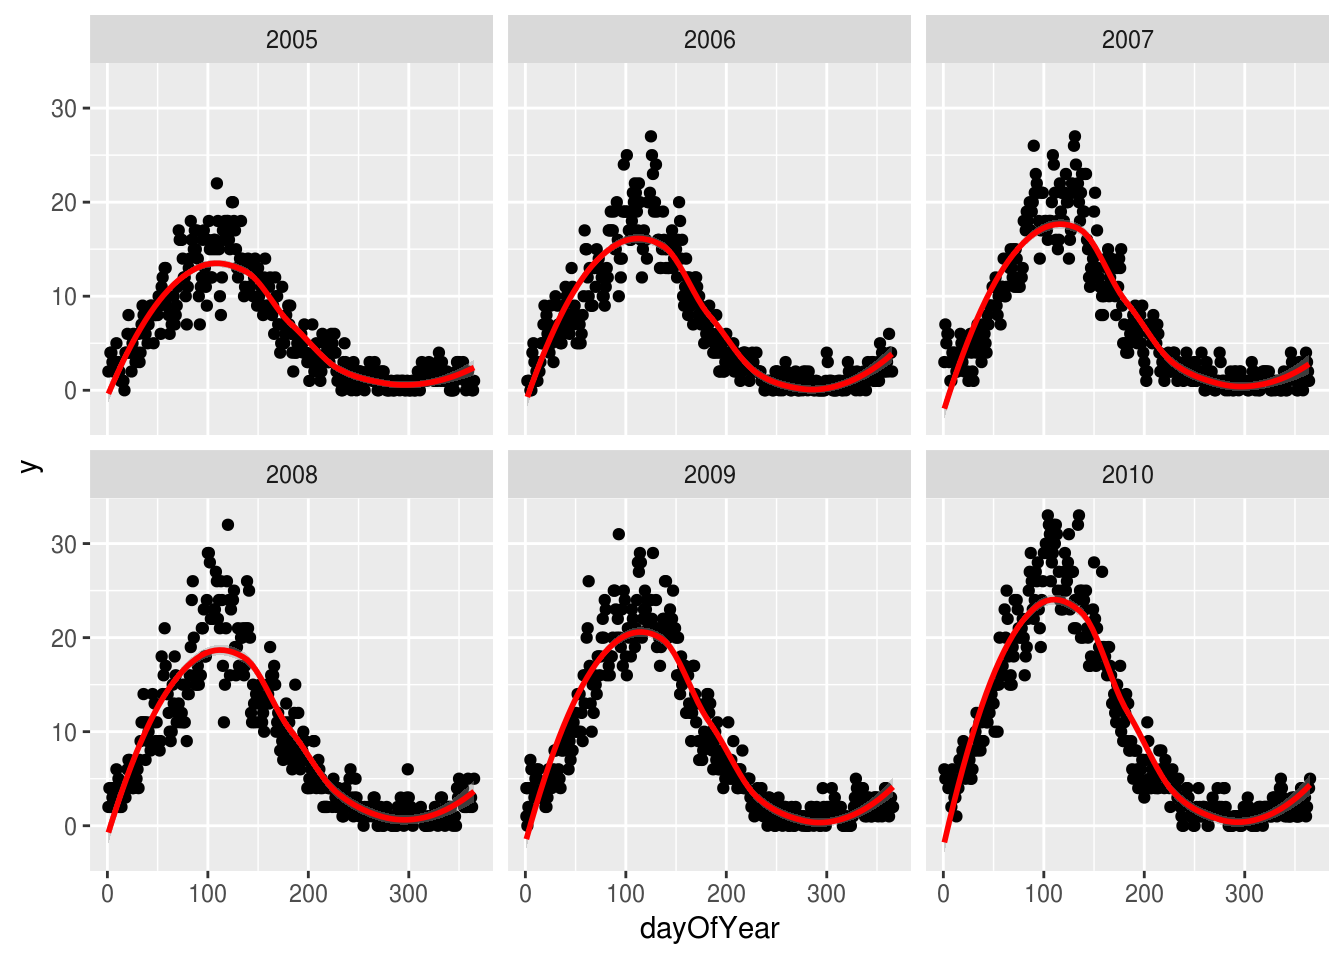
\includegraphics{website_files/figure-latex/unnamed-chunk-29-1.pdf}

\newpage

The Lomb-Scargle Periodogram shows a clear seasonality with a period of
365 days

\begin{verbatim}
// STATA CODE STARTS
insheet using "chapter_4.csv", clear

sort date
gen time=_n
tsset time, daily

wntestb y

cumsp y, gen(cumulative_spec_dist)
gen period=_N/_n

browse cumulative_spec_dist period
// STATA CODE ENDS
\end{verbatim}

\begin{Shaded}
\begin{Highlighting}[]
\CommentTok{# R CODE}
\NormalTok{lomb}\OperatorTok{::}\KeywordTok{lsp}\NormalTok{(d}\OperatorTok{$}\NormalTok{y,}\DataTypeTok{from=}\DecValTok{50}\NormalTok{,}\DataTypeTok{to=}\DecValTok{500}\NormalTok{,}\DataTypeTok{ofac=}\DecValTok{1}\NormalTok{,}\DataTypeTok{type=}\StringTok{"period"}\NormalTok{)}
\end{Highlighting}
\end{Shaded}

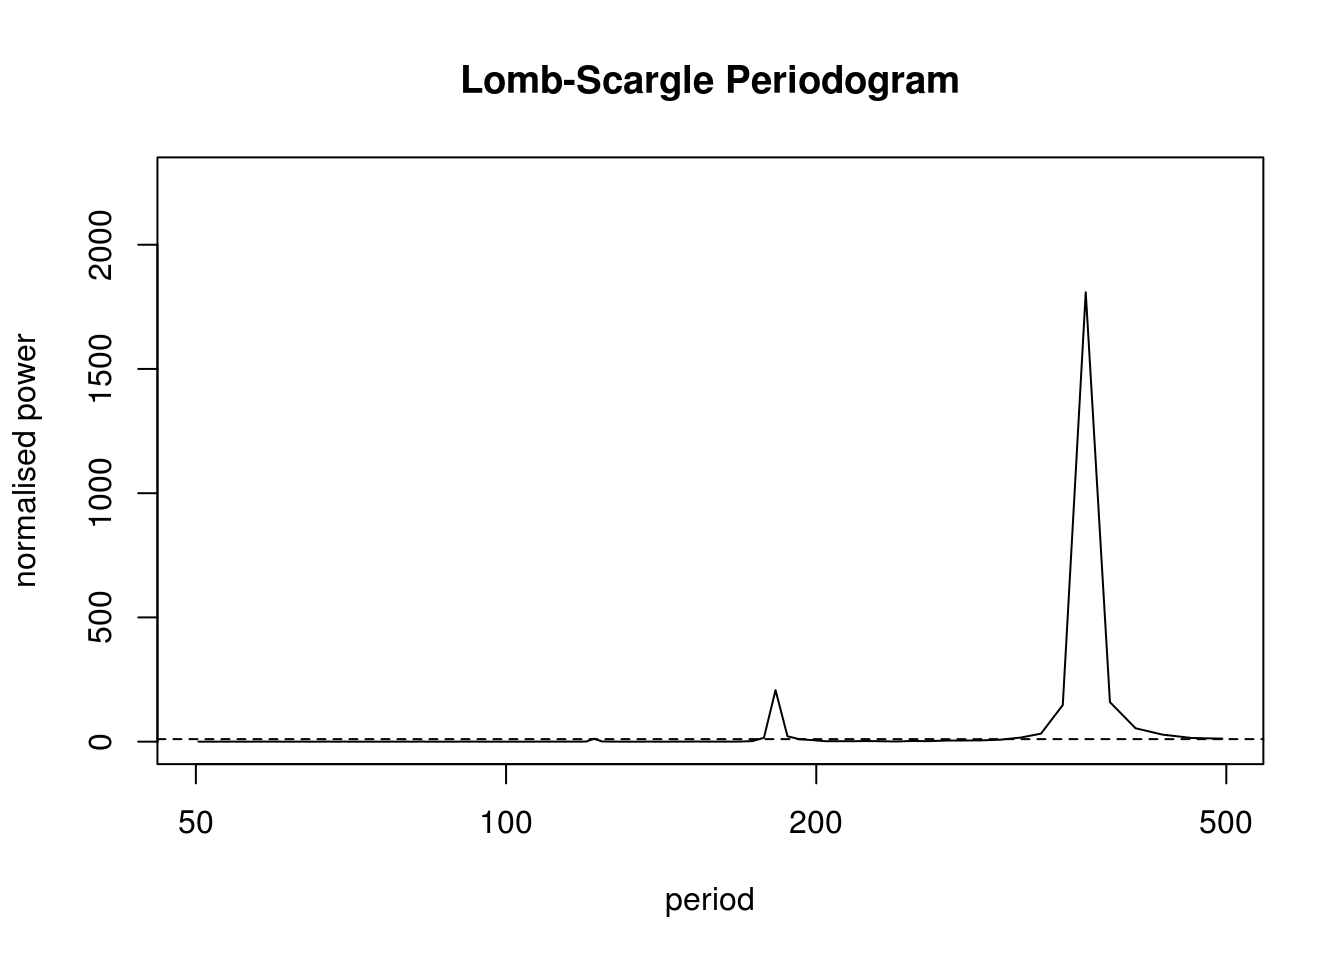
\includegraphics{website_files/figure-latex/unnamed-chunk-30-1.pdf}

\newpage

\section{Regressions}\label{regressions}

We then generate two new variables \texttt{cos365} and \texttt{sin365}
and perform a likelihood ratio test to see if they are significant or
not. This is done with two simple poisson regressions.

\begin{verbatim}
// STATA CODE STARTS
gen cos365=cos(dayofyear*2*_pi/365)
gen sin365=sin(dayofyear*2*_pi/365)

glm y yearminus2000, family(poisson)
estimates store m1
glm y yearminus2000 cos365 sin365, family(poisson)
estimates store m2

predict resid, anscombe

lrtest m1 m2
// STATA CODE ENDS
\end{verbatim}

\begin{Shaded}
\begin{Highlighting}[]
\CommentTok{# R CODE}
\NormalTok{d[,cos365}\OperatorTok{:}\ErrorTok{=}\KeywordTok{cos}\NormalTok{(dayOfYear}\OperatorTok{*}\DecValTok{2}\OperatorTok{*}\NormalTok{pi}\OperatorTok{/}\DecValTok{365}\NormalTok{)]}
\NormalTok{d[,sin365}\OperatorTok{:}\ErrorTok{=}\KeywordTok{sin}\NormalTok{(dayOfYear}\OperatorTok{*}\DecValTok{2}\OperatorTok{*}\NormalTok{pi}\OperatorTok{/}\DecValTok{365}\NormalTok{)]}

\NormalTok{fit0 <-}\StringTok{ }\KeywordTok{glm}\NormalTok{(y}\OperatorTok{~}\NormalTok{yearMinus2000, }\DataTypeTok{data=}\NormalTok{d, }\DataTypeTok{family=}\KeywordTok{poisson}\NormalTok{())}
\NormalTok{fit1 <-}\StringTok{ }\KeywordTok{glm}\NormalTok{(y}\OperatorTok{~}\NormalTok{yearMinus2000}\OperatorTok{+}\NormalTok{sin365 }\OperatorTok{+}\StringTok{ }\NormalTok{cos365, }\DataTypeTok{data=}\NormalTok{d, }\DataTypeTok{family=}\KeywordTok{poisson}\NormalTok{())}

\KeywordTok{print}\NormalTok{(lmtest}\OperatorTok{::}\KeywordTok{lrtest}\NormalTok{(fit0, fit1))}
\end{Highlighting}
\end{Shaded}

\begin{verbatim}
## Likelihood ratio test
## 
## Model 1: y ~ yearMinus2000
## Model 2: y ~ yearMinus2000 + sin365 + cos365
##   #Df LogLik Df Chisq Pr(>Chisq)    
## 1   2 -43124                        
## 2   4 -14542  2 57163  < 2.2e-16 ***
## ---
## Signif. codes:  0 '***' 0.001 '**' 0.01 '*' 0.05 '.' 0.1 ' ' 1
\end{verbatim}

We see that the likelihood ratio test for \texttt{sin365} and
\texttt{cos365} was significant, meaning that there is significant
seasonality with a 365 day periodicity in our data (which we already
strongly suspected due to the periodogram).

\newpage

We can now run/look at the results of our main regression.

\begin{Shaded}
\begin{Highlighting}[]
\KeywordTok{print}\NormalTok{(}\KeywordTok{summary}\NormalTok{(fit1))}
\end{Highlighting}
\end{Shaded}

\begin{verbatim}
## 
## Call:
## glm(formula = y ~ yearMinus2000 + sin365 + cos365, family = poisson(), 
##     data = d)
## 
## Deviance Residuals: 
##     Min       1Q   Median       3Q      Max  
## -2.6774  -0.6738  -0.0503   0.4920   3.5820  
## 
## Coefficients:
##                 Estimate Std. Error z value Pr(>|z|)    
## (Intercept)    0.7981246  0.0105300   75.80   <2e-16 ***
## yearMinus2000  0.0991480  0.0007416  133.70   <2e-16 ***
## sin365         1.4074818  0.0073418  191.71   <2e-16 ***
## cos365        -0.5390314  0.0061513  -87.63   <2e-16 ***
## ---
## Signif. codes:  0 '***' 0.001 '**' 0.01 '*' 0.05 '.' 0.1 ' ' 1
## 
## (Dispersion parameter for poisson family taken to be 1)
## 
##     Null deviance: 81832.6  on 6939  degrees of freedom
## Residual deviance:  5217.8  on 6936  degrees of freedom
## AIC: 29093
## 
## Number of Fisher Scoring iterations: 4
\end{verbatim}

We also see that the coefficient for year is \texttt{0.1} which means
that for each additional year, the outcome increases by
\texttt{exp(0.1)=1.11}.

\newpage

\section{Residual analysis}\label{residual-analysis}

\begin{Shaded}
\begin{Highlighting}[]
\NormalTok{d[,residuals}\OperatorTok{:}\ErrorTok{=}\KeywordTok{residuals}\NormalTok{(fit1, }\DataTypeTok{type =} \StringTok{"response"}\NormalTok{)]}
\NormalTok{d[,predicted}\OperatorTok{:}\ErrorTok{=}\KeywordTok{predict}\NormalTok{(fit1, }\DataTypeTok{type =} \StringTok{"response"}\NormalTok{)]}
\end{Highlighting}
\end{Shaded}

We can see a clear \texttt{AR(1)} pattern in our residuals.

\begin{verbatim}
// STATA CODE STARTS
pac resid
// STATA CODE ENDS
\end{verbatim}

\begin{Shaded}
\begin{Highlighting}[]
\CommentTok{# R CODE}
\CommentTok{# this is for AR}
\KeywordTok{pacf}\NormalTok{(d}\OperatorTok{$}\NormalTok{residuals)}
\end{Highlighting}
\end{Shaded}

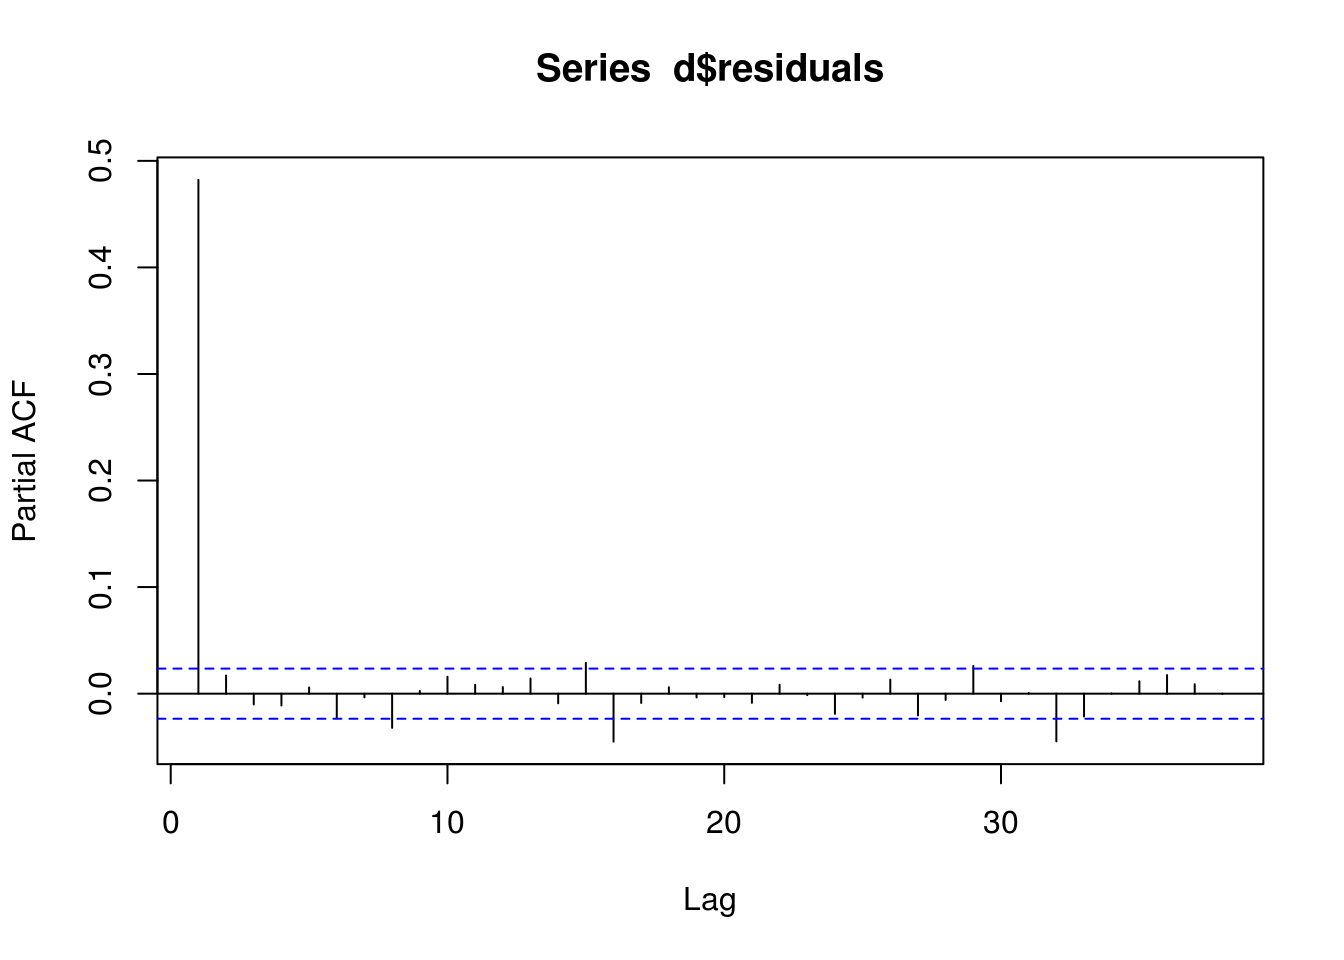
\includegraphics{website_files/figure-latex/unnamed-chunk-34-1.pdf}

\newpage

And again we see some sort of \texttt{AR} pattern in our residuals.

\begin{verbatim}
// STATA CODE STARTS
ac resid
// STATA CODE ENDS
\end{verbatim}

\begin{Shaded}
\begin{Highlighting}[]
\CommentTok{# R CODE}
\CommentTok{# this is for MA}
\KeywordTok{acf}\NormalTok{(d}\OperatorTok{$}\NormalTok{residuals)}
\end{Highlighting}
\end{Shaded}

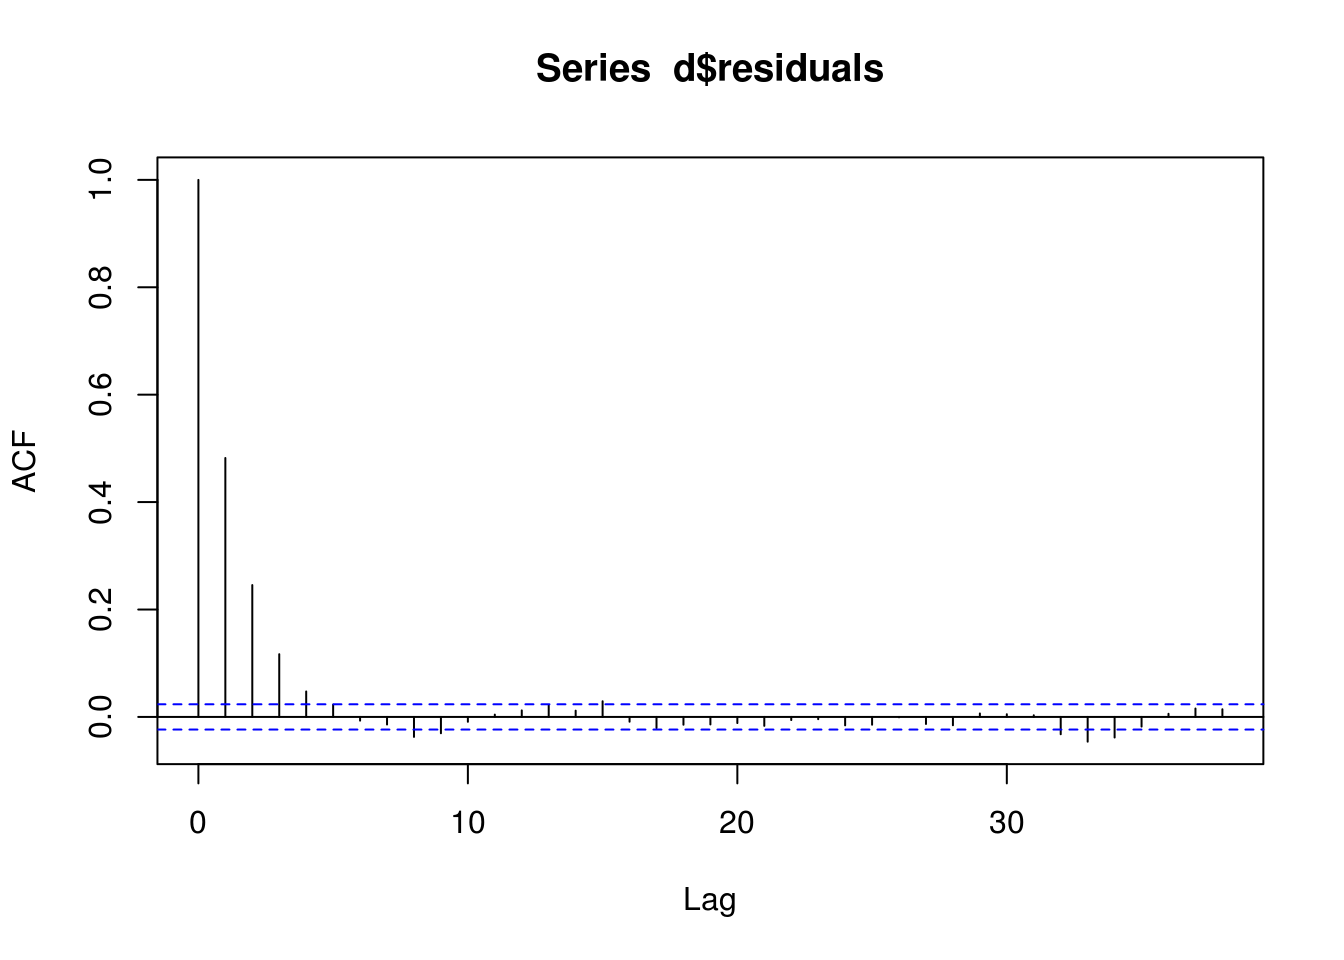
\includegraphics{website_files/figure-latex/unnamed-chunk-35-1.pdf}

This means our model is bad, we have autocorrelation. We now need to
change our model to account for this \texttt{AR(1)} autocorrelation!

\newpage

\section{(R ONLY) Regression with AR(1) correlation in
residuals}\label{r-only-regression-with-ar1-correlation-in-residuals}

First we create an \texttt{id} variable. This generally corresponds to
geographical locations, or people. In this case, we only have one
geographical location, so our \texttt{id} for all observations is
\texttt{1}. This lets the computer know that all data belongs to the
same group.

When we have autocorrelation in the residuals, we can use the
\texttt{MASS::glmPQL} function in R.

\begin{Shaded}
\begin{Highlighting}[]
\NormalTok{d[,ID}\OperatorTok{:}\ErrorTok{=}\DecValTok{1}\NormalTok{]}
\CommentTok{# this is for MA}
\NormalTok{fit <-}\StringTok{ }\NormalTok{MASS}\OperatorTok{::}\KeywordTok{glmmPQL}\NormalTok{(y}\OperatorTok{~}\NormalTok{yearMinus2000}\OperatorTok{+}\NormalTok{sin365 }\OperatorTok{+}\StringTok{ }\NormalTok{cos365, }\DataTypeTok{random =} \OperatorTok{~}\StringTok{ }\DecValTok{1} \OperatorTok{|}\StringTok{ }\NormalTok{ID,}
                \DataTypeTok{family =}\NormalTok{ poisson, }\DataTypeTok{data =}\NormalTok{ d,}
                \DataTypeTok{correlation=}\NormalTok{nlme}\OperatorTok{::}\KeywordTok{corAR1}\NormalTok{(}\DataTypeTok{form=}\OperatorTok{~}\NormalTok{dayOfSeries}\OperatorTok{|}\NormalTok{ID))}
\end{Highlighting}
\end{Shaded}

\begin{verbatim}
## iteration 1
\end{verbatim}

\begin{Shaded}
\begin{Highlighting}[]
\KeywordTok{summary}\NormalTok{(fit)}
\end{Highlighting}
\end{Shaded}

\begin{verbatim}
## Linear mixed-effects model fit by maximum likelihood
##  Data: d 
##   AIC BIC logLik
##    NA  NA     NA
## 
## Random effects:
##  Formula: ~1 | ID
##          (Intercept) Residual
## StdDev: 1.149087e-05 0.841689
## 
## Correlation Structure: AR(1)
##  Formula: ~dayOfSeries | ID 
##  Parameter estimate(s):
##       Phi 
## 0.4926123 
## Variance function:
##  Structure: fixed weights
##  Formula: ~invwt 
## Fixed effects: y ~ yearMinus2000 + sin365 + cos365 
##                    Value   Std.Error   DF   t-value p-value
## (Intercept)    0.7980540 0.015203158 6936  52.49265       0
## yearMinus2000  0.0991582 0.001070583 6936  92.62077       0
## sin365         1.4074339 0.010596650 6936 132.81876       0
## cos365        -0.5389807 0.008876448 6936 -60.72031       0
##  Correlation: 
##               (Intr) yM2000 sin365
## yearMinus2000 -0.832              
## sin365        -0.409  0.000       
## cos365         0.186  0.000 -0.158
## 
## Standardized Within-Group Residuals:
##         Min          Q1         Med          Q3         Max 
## -2.89886750 -0.75775061 -0.05982255  0.60730689  6.49964489 
## 
## Number of Observations: 6940
## Number of Groups: 1
\end{verbatim}

\newpage 

We can see that the residuals no longer display any signs of
autocorrelation.

\begin{Shaded}
\begin{Highlighting}[]
\KeywordTok{pacf}\NormalTok{(}\KeywordTok{residuals}\NormalTok{(fit, }\DataTypeTok{type =} \StringTok{"normalized"}\NormalTok{)) }\CommentTok{# this is for AR}
\end{Highlighting}
\end{Shaded}

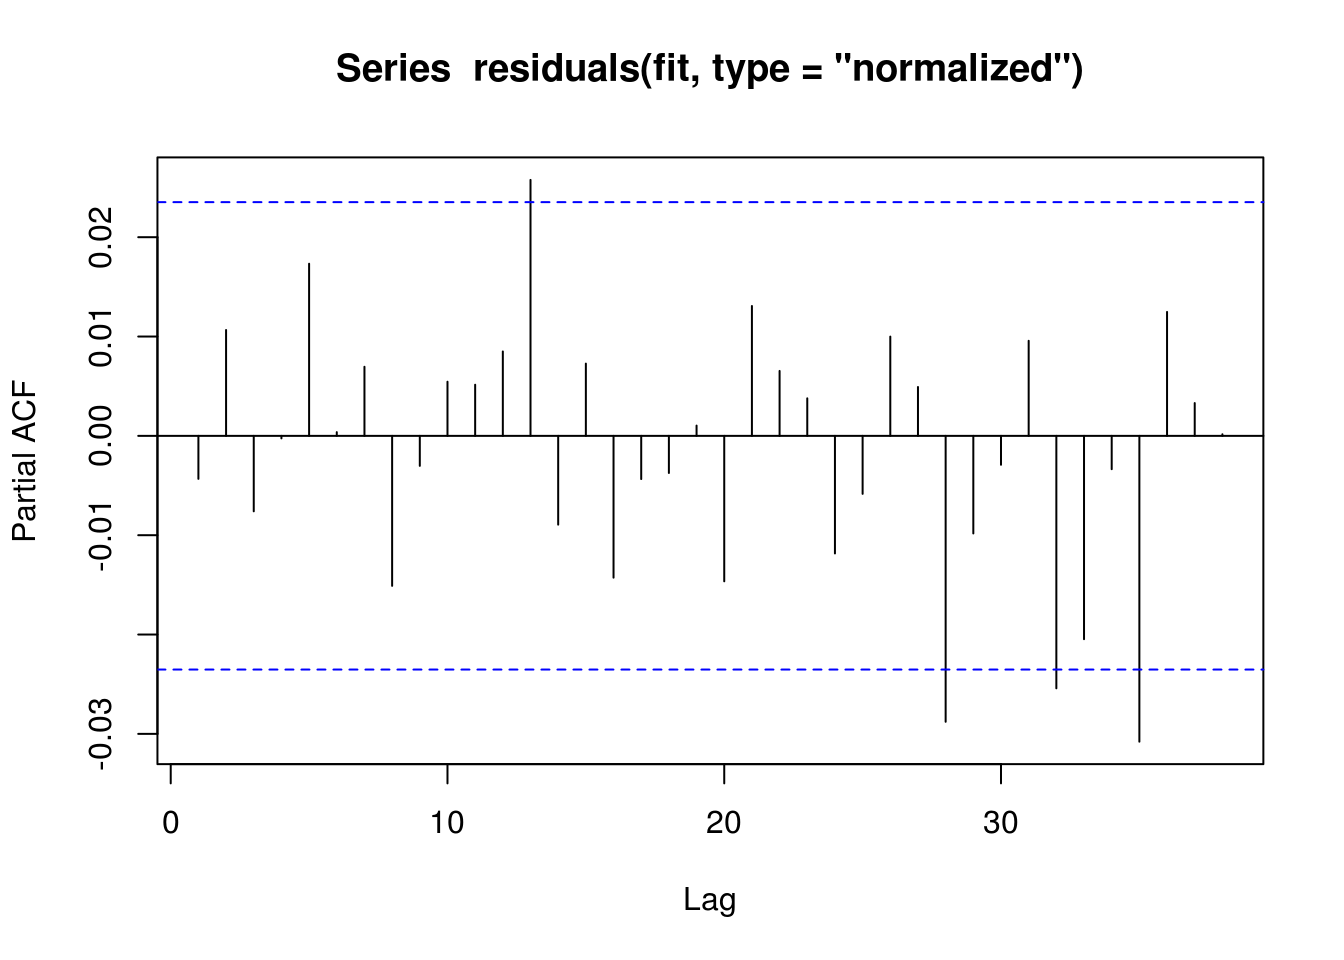
\includegraphics{website_files/figure-latex/unnamed-chunk-37-1.pdf}

\newpage

We can see that the residuals no longer display any signs of
autocorrelation.

\begin{Shaded}
\begin{Highlighting}[]
\KeywordTok{acf}\NormalTok{(}\KeywordTok{residuals}\NormalTok{(fit, }\DataTypeTok{type =} \StringTok{"normalized"}\NormalTok{)) }\CommentTok{# this is for MA}
\end{Highlighting}
\end{Shaded}

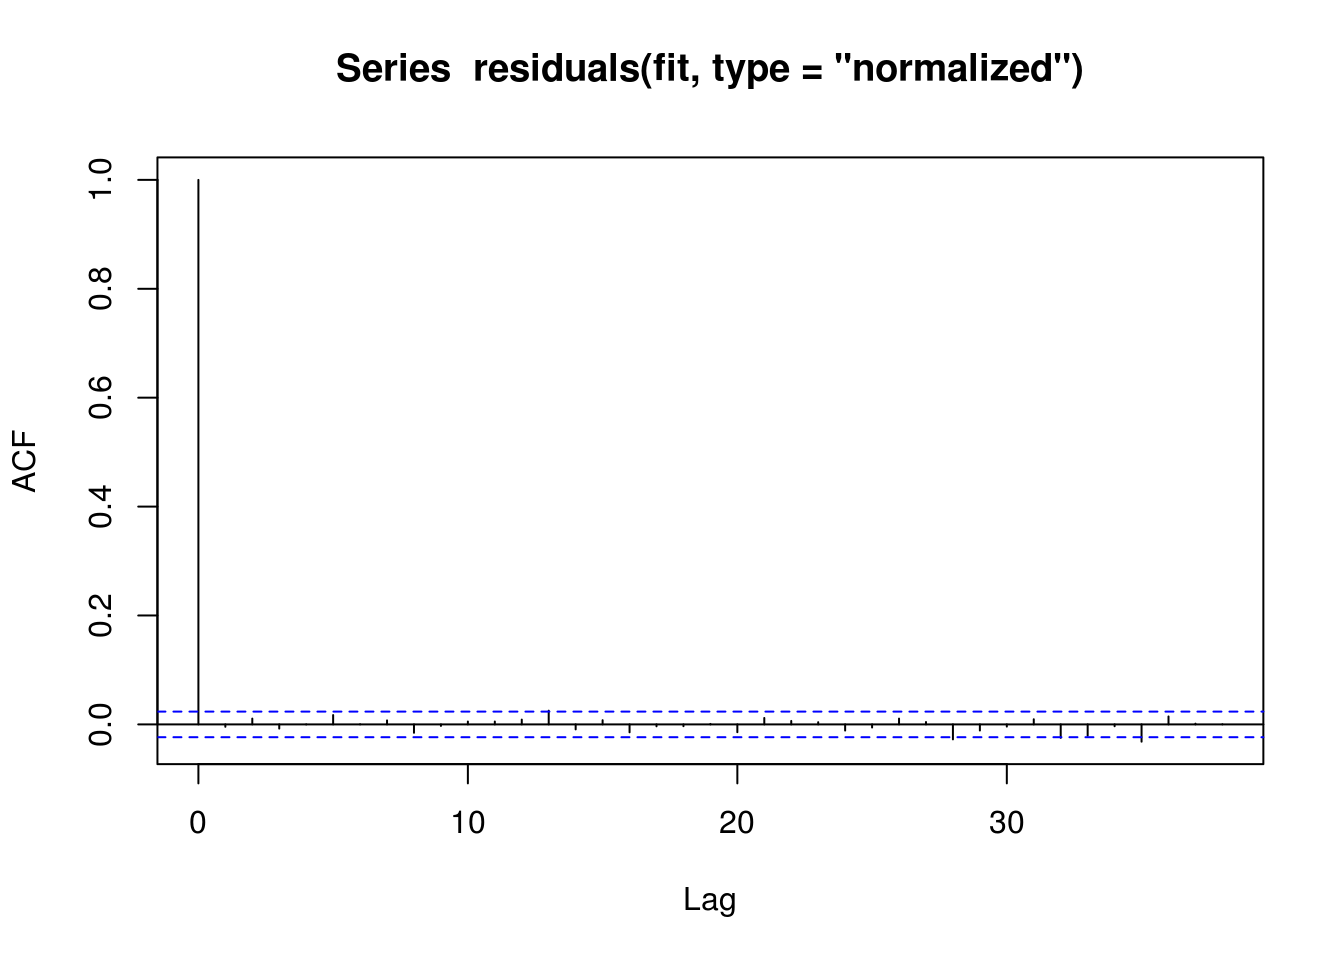
\includegraphics{website_files/figure-latex/unnamed-chunk-38-1.pdf}

\newpage

We also obtain the same estimates that we did in the last chapter.

\begin{Shaded}
\begin{Highlighting}[]
\NormalTok{b1 <-}\StringTok{ }\FloatTok{1.3936185} \CommentTok{# sin coefficient}
\NormalTok{b2 <-}\StringTok{ }\OperatorTok{-}\FloatTok{0.5233866} \CommentTok{# cos coefficient}
\NormalTok{amplitude <-}\StringTok{ }\KeywordTok{sqrt}\NormalTok{(b1}\OperatorTok{^}\DecValTok{2} \OperatorTok{+}\StringTok{ }\NormalTok{b2}\OperatorTok{^}\DecValTok{2}\NormalTok{)}
\NormalTok{p <-}\StringTok{ }\KeywordTok{atan}\NormalTok{(b1}\OperatorTok{/}\NormalTok{b2) }\OperatorTok{*}\StringTok{ }\DecValTok{365}\OperatorTok{/}\DecValTok{2}\OperatorTok{/}\NormalTok{pi}
\ControlFlowTok{if}\NormalTok{ (p }\OperatorTok{>}\StringTok{ }\DecValTok{0}\NormalTok{) \{}
\NormalTok{    peak <-}\StringTok{ }\NormalTok{p}
\NormalTok{    trough <-}\StringTok{ }\NormalTok{p }\OperatorTok{+}\StringTok{ }\DecValTok{365}\OperatorTok{/}\DecValTok{2}
\NormalTok{\} }\ControlFlowTok{else}\NormalTok{ \{}
\NormalTok{    peak <-}\StringTok{ }\NormalTok{p }\OperatorTok{+}\StringTok{ }\DecValTok{365}\OperatorTok{/}\DecValTok{2}
\NormalTok{    trough <-}\StringTok{ }\NormalTok{p }\OperatorTok{+}\StringTok{ }\DecValTok{365}
\NormalTok{\}}
\ControlFlowTok{if}\NormalTok{ (b1 }\OperatorTok{<}\StringTok{ }\DecValTok{0}\NormalTok{) \{}
\NormalTok{    g <-}\StringTok{ }\NormalTok{peak}
\NormalTok{    peak <-}\StringTok{ }\NormalTok{trough}
\NormalTok{    trough <-}\StringTok{ }\NormalTok{g}
\NormalTok{\}}
\KeywordTok{print}\NormalTok{(}\KeywordTok{sprintf}\NormalTok{(}\StringTok{"amplitude is estimated as %s, peak is estimated as %s, trough is estimated as %s"}\NormalTok{,}\KeywordTok{round}\NormalTok{(amplitude,}\DecValTok{2}\NormalTok{),}\KeywordTok{round}\NormalTok{(peak),}\KeywordTok{round}\NormalTok{(trough)))}
\end{Highlighting}
\end{Shaded}

\begin{verbatim}
## [1] "amplitude is estimated as 1.49, peak is estimated as 112, trough is estimated as 295"
\end{verbatim}

\begin{Shaded}
\begin{Highlighting}[]
\KeywordTok{print}\NormalTok{(}\KeywordTok{sprintf}\NormalTok{(}\StringTok{"true values are: amplitude: %s, peak: %s, trough: %s"}\NormalTok{,}\KeywordTok{round}\NormalTok{(AMPLITUDE,}\DecValTok{2}\NormalTok{),}\KeywordTok{round}\NormalTok{(}\DecValTok{365}\OperatorTok{/}\DecValTok{4}\OperatorTok{+}\NormalTok{SEASONAL_HORIZONTAL_SHIFT),}\KeywordTok{round}\NormalTok{(}\DecValTok{3}\OperatorTok{*}\DecValTok{365}\OperatorTok{/}\DecValTok{4}\OperatorTok{+}\NormalTok{SEASONAL_HORIZONTAL_SHIFT)))}
\end{Highlighting}
\end{Shaded}

\begin{verbatim}
## [1] "true values are: amplitude: 1.5, peak: 111, trough: 294"
\end{verbatim}

\newpage

\section{(STATA ONLY) Regression with robust standard
errors}\label{stata-only-regression-with-robust-standard-errors}

In STATA it is not possible to explicitly model autocorrelation in the
residuals (with the exception of linear regression). Since most of our
work deals with logistic and poisson regressions, we will be focusing on
modelling strategies that work with all kinds of regressions.

The STATA approach to autocorrelation is to estimate more
\texttt{robust} standard errors. That is, STATA makes the standard
errors larger to account for the model mispecification. This is done
through the \texttt{vce(robust)} option.

\begin{verbatim}
// STATA CODE STARTS
glm y yearminus2000 cos365 sin365, family(poisson) vce(robust)
// STATA CODE ENDS
\end{verbatim}

\chapter{Not panel data: Multiple
areas}\label{not-panel-data-multiple-areas}

\section{Aim}\label{aim-2}

We are given a dataset containing counts of diseases from multiple
geographical areas. We want to identify:

\begin{itemize}
\tightlist
\item
  Is there a general yearly trend (i.e.~increasing or decreasing from
  year to year?)
\item
  Is variable \texttt{x} associated with the outcome?
\end{itemize}

\newpage

\section{Creating the data}\label{creating-the-data-2}

The data for this chapter is available at:
\url{http://rwhite.no/longitudinal_analysis/data/chapter_5.csv}

\begin{Shaded}
\begin{Highlighting}[]
\KeywordTok{library}\NormalTok{(data.table)}
\KeywordTok{library}\NormalTok{(lme4)}
\end{Highlighting}
\end{Shaded}

\begin{verbatim}
## Loading required package: Matrix
\end{verbatim}

\begin{Shaded}
\begin{Highlighting}[]
\KeywordTok{set.seed}\NormalTok{(}\DecValTok{4}\NormalTok{)}

\NormalTok{fylkeIntercepts <-}\StringTok{ }\KeywordTok{data.table}\NormalTok{(}\DataTypeTok{fylke=}\DecValTok{1}\OperatorTok{:}\DecValTok{20}\NormalTok{,}\DataTypeTok{fylkeIntercepts=}\KeywordTok{rnorm}\NormalTok{(}\DecValTok{20}\NormalTok{))}

\NormalTok{d <-}\StringTok{ }\KeywordTok{data.table}\NormalTok{(}\DataTypeTok{fylke=}\KeywordTok{rep}\NormalTok{(}\DecValTok{1}\OperatorTok{:}\DecValTok{20}\NormalTok{,}\DataTypeTok{each=}\DecValTok{100}\NormalTok{))}
\NormalTok{d <-}\StringTok{ }\KeywordTok{merge}\NormalTok{(d,fylkeIntercepts,}\DataTypeTok{by=}\StringTok{"fylke"}\NormalTok{)}
\NormalTok{d[,mainIntercept}\OperatorTok{:}\ErrorTok{=}\DecValTok{3}\NormalTok{]}
\NormalTok{d[,x}\OperatorTok{:}\ErrorTok{=}\KeywordTok{runif}\NormalTok{(.N)]}
\NormalTok{d[,year}\OperatorTok{:}\ErrorTok{=}\KeywordTok{sample}\NormalTok{(}\KeywordTok{c}\NormalTok{(}\DecValTok{1950}\OperatorTok{:}\DecValTok{2018}\NormalTok{),.N,}\DataTypeTok{replace=}\NormalTok{T)]}
\NormalTok{d[,mu }\OperatorTok{:}\ErrorTok{=}\StringTok{ }\KeywordTok{exp}\NormalTok{(mainIntercept }\OperatorTok{+}\StringTok{ }\NormalTok{fylkeIntercepts }\OperatorTok{+}\StringTok{ }\DecValTok{3}\OperatorTok{*}\NormalTok{x)]}
\NormalTok{d[,y}\OperatorTok{:}\ErrorTok{=}\KeywordTok{rpois}\NormalTok{(.N,mu)]}

\KeywordTok{fwrite}\NormalTok{(d,}\StringTok{"data/chapter_5.csv"}\NormalTok{)}
\end{Highlighting}
\end{Shaded}

\newpage

\section{Investigating the data}\label{investigating-the-data}

We can see from the data that we have 20 geographical areas
(\texttt{fylke}) with 100 observations for each fylke, but the sampling
did not happen consistently (some years have multiple measurements,
other years have no measurements).

This means we have:

\begin{itemize}
\tightlist
\item
  multiple geographical areas
\item
  multiple observations in each geographical area
\item
  not panel data
\end{itemize}

\begin{Shaded}
\begin{Highlighting}[]
\KeywordTok{print}\NormalTok{(d)}
\end{Highlighting}
\end{Shaded}

\begin{verbatim}
##       fylke fylkeIntercepts mainIntercept          x year        mu   y
##    1:     1       0.2167549             3 0.93831909 1966 416.42739 392
##    2:     1       0.2167549             3 0.24217109 1981  51.58692  51
##    3:     1       0.2167549             3 0.56559453 1972 136.12022 135
##    4:     1       0.2167549             3 0.18089910 1950  42.92490  39
##    5:     1       0.2167549             3 0.90449929 1951 376.24959 367
##   ---                                                                  
## 1996:    20      -0.2834446             3 0.89237059 1995 220.00872 209
## 1997:    20      -0.2834446             3 0.80522348 2006 169.39375 157
## 1998:    20      -0.2834446             3 0.59989167 1955  91.49007  96
## 1999:    20      -0.2834446             3 0.04148228 1996  17.13293  18
## 2000:    20      -0.2834446             3 0.77673920 2002 155.51980 152
\end{verbatim}

\newpage

\section{Regression}\label{regression}

For this scenario, we use the \texttt{lme4::glmer} function in R. We
need to introduce a \texttt{(1\textbar{}fylke)} term to identify the
geographical areas (i.e.~clusters). In STATA we use the \texttt{meglm}
function and introduce a \texttt{\textbar{}\textbar{}\ fylke:} term to
identify the geographical areas (i.e.~clusters).

\begin{verbatim}
// STATA CODE STARTS
insheet using "chapter_5.csv", clear

gen yearMinus2000 = year-2000
meglm y x yearMinus2000 || fylke:, family(poisson)
// STATA CODE ENDS
\end{verbatim}

\begin{Shaded}
\begin{Highlighting}[]
\CommentTok{# R CODE}
\NormalTok{d[,yearMinus2000}\OperatorTok{:}\ErrorTok{=}\NormalTok{year}\OperatorTok{-}\DecValTok{2000}\NormalTok{]}
\KeywordTok{summary}\NormalTok{(fit <-}\StringTok{ }\NormalTok{lme4}\OperatorTok{::}\KeywordTok{glmer}\NormalTok{(y}\OperatorTok{~}\NormalTok{x }\OperatorTok{+}\StringTok{ }\NormalTok{yearMinus2000 }\OperatorTok{+}\StringTok{ }\NormalTok{(}\DecValTok{1}\OperatorTok{|}\NormalTok{fylke),}\DataTypeTok{data=}\NormalTok{d,}\DataTypeTok{family=}\KeywordTok{poisson}\NormalTok{()))}
\end{Highlighting}
\end{Shaded}

\begin{verbatim}
## Generalized linear mixed model fit by maximum likelihood (Laplace
##   Approximation) [glmerMod]
##  Family: poisson  ( log )
## Formula: y ~ x + yearMinus2000 + (1 | fylke)
##    Data: d
## 
##      AIC      BIC   logLik deviance df.resid 
##  15415.5  15437.9  -7703.8  15407.5     1996 
## 
## Scaled residuals: 
##     Min      1Q  Median      3Q     Max 
## -3.0448 -0.6432 -0.0067  0.6452  4.2338 
## 
## Random effects:
##  Groups Name        Variance Std.Dev.
##  fylke  (Intercept) 0.6114   0.7819  
## Number of obs: 2000, groups:  fylke, 20
## 
## Fixed effects:
##                 Estimate Std. Error z value Pr(>|z|)    
## (Intercept)    3.375e+00  1.749e-01  19.295   <2e-16 ***
## x              3.002e+00  5.994e-03 500.874   <2e-16 ***
## yearMinus2000 -9.943e-07  7.192e-05  -0.014    0.989    
## ---
## Signif. codes:  0 '***' 0.001 '**' 0.01 '*' 0.05 '.' 0.1 ' ' 1
## 
## Correlation of Fixed Effects:
##             (Intr) x     
## x           -0.025       
## yearMns2000  0.007 -0.030
## convergence code: 0
## Model is nearly unidentifiable: very large eigenvalue
##  - Rescale variables?
## Model is nearly unidentifiable: large eigenvalue ratio
##  - Rescale variables?
\end{verbatim}

You can see that the format of the results is the same as an ordinary
regression.

\chapter{Panel data: multiple areas without
autocorrelation}\label{panel-data-multiple-areas-without-autocorrelation}

\section{Aim}\label{aim-3}

We are given a dataset containing daily counts of diseases from multiple
geographical areas. We want to identify:

\begin{itemize}
\tightlist
\item
  Does seasonality exist?
\item
  If seasonality exists, when are the high/low seasons?
\item
  Is there a general yearly trend (i.e.~increasing or decreasing from
  year to year?)
\end{itemize}

\newpage

\section{Creating the data}\label{creating-the-data-3}

The data for this chapter is available at:
\url{http://rwhite.no/longitudinal_analysis/data/chapter_6.csv}

\begin{Shaded}
\begin{Highlighting}[]
\KeywordTok{library}\NormalTok{(data.table)}
\KeywordTok{library}\NormalTok{(ggplot2)}
\KeywordTok{set.seed}\NormalTok{(}\DecValTok{4}\NormalTok{)}

\NormalTok{AMPLITUDE <-}\StringTok{ }\FloatTok{1.5}
\NormalTok{SEASONAL_HORIZONTAL_SHIFT <-}\StringTok{ }\DecValTok{20}

\NormalTok{fylkeIntercepts <-}\StringTok{ }\KeywordTok{data.table}\NormalTok{(}\DataTypeTok{fylke=}\DecValTok{1}\OperatorTok{:}\DecValTok{20}\NormalTok{,}\DataTypeTok{fylkeIntercepts=}\KeywordTok{rnorm}\NormalTok{(}\DecValTok{20}\NormalTok{))}

\NormalTok{d <-}\StringTok{ }\KeywordTok{data.table}\NormalTok{(}\DataTypeTok{date=}\KeywordTok{seq.Date}\NormalTok{(}
  \DataTypeTok{from=}\KeywordTok{as.Date}\NormalTok{(}\StringTok{"2010-01-01"}\NormalTok{),}
  \DataTypeTok{to=}\KeywordTok{as.Date}\NormalTok{(}\StringTok{"2015-12-31"}\NormalTok{),}
  \DataTypeTok{by=}\DecValTok{1}\NormalTok{))}
\NormalTok{d[,year}\OperatorTok{:}\ErrorTok{=}\KeywordTok{as.numeric}\NormalTok{(}\KeywordTok{format.Date}\NormalTok{(date,}\StringTok{"%G"}\NormalTok{))]}
\NormalTok{d[,week}\OperatorTok{:}\ErrorTok{=}\KeywordTok{as.numeric}\NormalTok{(}\KeywordTok{format.Date}\NormalTok{(date,}\StringTok{"%V"}\NormalTok{))]}
\NormalTok{d[,month}\OperatorTok{:}\ErrorTok{=}\KeywordTok{as.numeric}\NormalTok{(}\KeywordTok{format.Date}\NormalTok{(date,}\StringTok{"%m"}\NormalTok{))]}

\NormalTok{temp <-}\StringTok{ }\KeywordTok{vector}\NormalTok{(}\StringTok{"list"}\NormalTok{,}\DataTypeTok{length=}\DecValTok{20}\NormalTok{)}
\ControlFlowTok{for}\NormalTok{(i }\ControlFlowTok{in} \DecValTok{1}\OperatorTok{:}\DecValTok{20}\NormalTok{)\{}
\NormalTok{  temp[[i]] <-}\StringTok{ }\KeywordTok{copy}\NormalTok{(d)}
\NormalTok{  temp[[i]][,fylke}\OperatorTok{:}\ErrorTok{=}\NormalTok{i]}
\NormalTok{\}}
\NormalTok{d <-}\StringTok{ }\KeywordTok{rbindlist}\NormalTok{(temp)}

\NormalTok{d[,yearMinus2000}\OperatorTok{:}\ErrorTok{=}\NormalTok{year}\OperatorTok{-}\DecValTok{2000}\NormalTok{]}
\NormalTok{d[,dayOfSeries}\OperatorTok{:}\ErrorTok{=}\DecValTok{1}\OperatorTok{:}\NormalTok{.N]}

\NormalTok{d[,dayOfYear}\OperatorTok{:}\ErrorTok{=}\KeywordTok{as.numeric}\NormalTok{(}\KeywordTok{format.Date}\NormalTok{(date,}\StringTok{"%j"}\NormalTok{))]}
\NormalTok{d[,seasonalEffect}\OperatorTok{:}\ErrorTok{=}\KeywordTok{sin}\NormalTok{(}\DecValTok{2}\OperatorTok{*}\NormalTok{pi}\OperatorTok{*}\NormalTok{(dayOfYear}\OperatorTok{-}\NormalTok{SEASONAL_HORIZONTAL_SHIFT)}\OperatorTok{/}\DecValTok{365}\NormalTok{)]}
\NormalTok{d[,mu }\OperatorTok{:}\ErrorTok{=}\StringTok{ }\KeywordTok{exp}\NormalTok{(}\FloatTok{0.1} \OperatorTok{+}\StringTok{ }\NormalTok{yearMinus2000}\OperatorTok{*}\FloatTok{0.1} \OperatorTok{+}\StringTok{ }\NormalTok{seasonalEffect}\OperatorTok{*}\NormalTok{AMPLITUDE)]}
\NormalTok{d[,y}\OperatorTok{:}\ErrorTok{=}\KeywordTok{rpois}\NormalTok{(.N,mu)]}

\KeywordTok{fwrite}\NormalTok{(d,}\StringTok{"data/chapter_6.csv"}\NormalTok{)}
\end{Highlighting}
\end{Shaded}

\newpage

\section{Investigation}\label{investigation-2}

We then drill down into a few years for fylke 1, and see a clear
seasonal trend

\begin{Shaded}
\begin{Highlighting}[]
\NormalTok{q <-}\StringTok{ }\KeywordTok{ggplot}\NormalTok{(d[fylke}\OperatorTok{==}\DecValTok{1}\NormalTok{],}\KeywordTok{aes}\NormalTok{(}\DataTypeTok{x=}\NormalTok{dayOfYear,}\DataTypeTok{y=}\NormalTok{y))}
\NormalTok{q <-}\StringTok{ }\NormalTok{q }\OperatorTok{+}\StringTok{ }\KeywordTok{facet_wrap}\NormalTok{(}\OperatorTok{~}\NormalTok{year)}
\NormalTok{q <-}\StringTok{ }\NormalTok{q }\OperatorTok{+}\StringTok{ }\KeywordTok{geom_point}\NormalTok{()}
\NormalTok{q <-}\StringTok{ }\NormalTok{q }\OperatorTok{+}\StringTok{ }\KeywordTok{stat_smooth}\NormalTok{(}\DataTypeTok{colour=}\StringTok{"red"}\NormalTok{)}
\NormalTok{q}
\end{Highlighting}
\end{Shaded}

\begin{verbatim}
## `geom_smooth()` using method = 'loess' and formula 'y ~ x'
\end{verbatim}

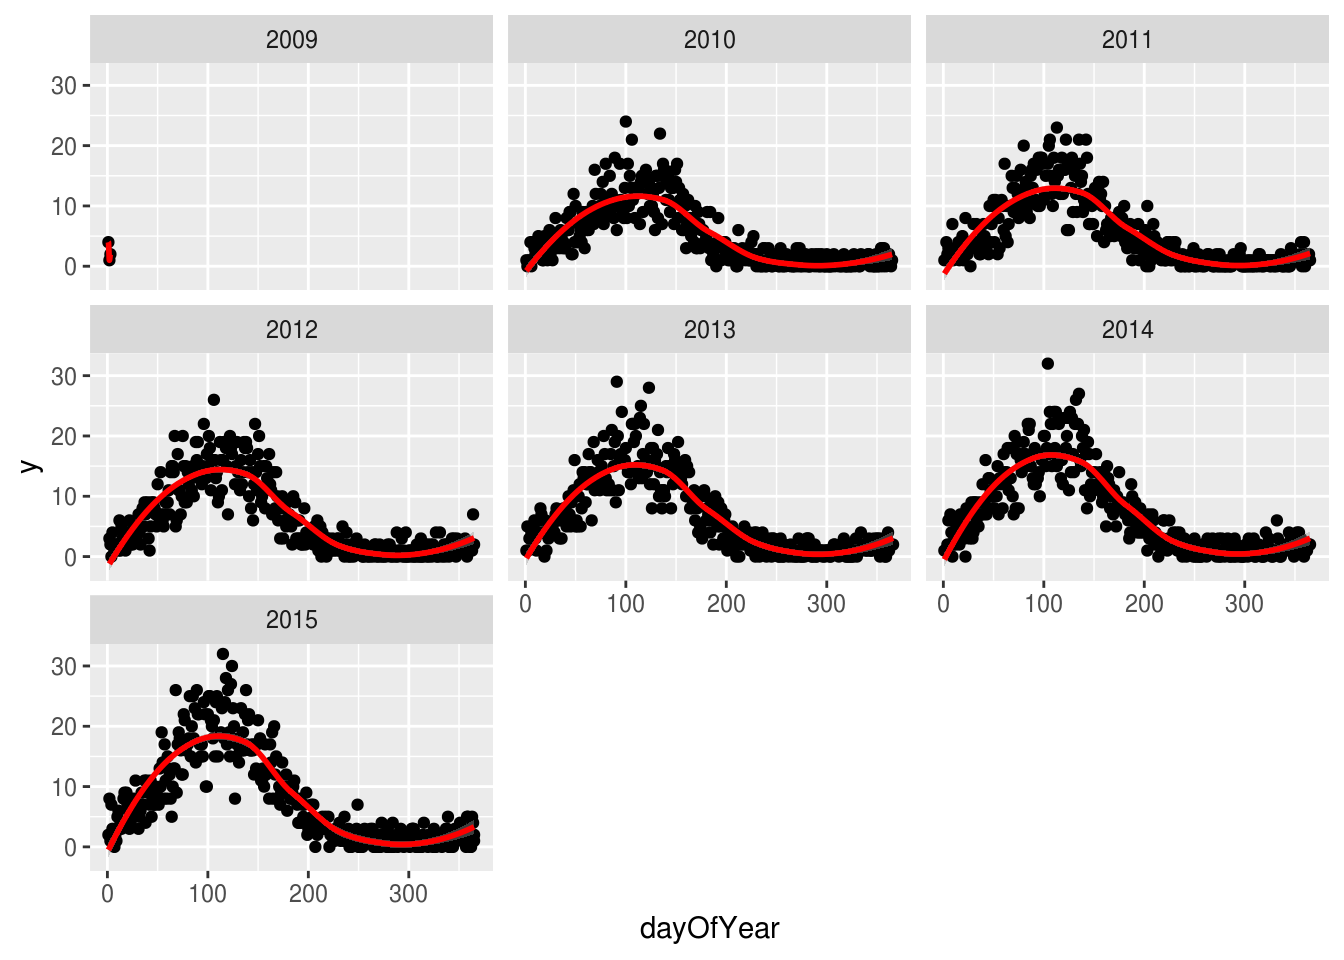
\includegraphics{website_files/figure-latex/unnamed-chunk-44-1.pdf}

\newpage

The Lomb-Scargle Periodogram shows a clear seasonality with a period of
365 days

\begin{verbatim}
// STATA CODE STARTS
insheet using "chapter_6.csv", clear

sort fylke date
by fylke: gen time=_n
tsset fylke time, daily

wntestb y if fylke==1

cumsp y if fylke==1, gen(cumulative_spec_dist)
by fylke: gen period=_N/_n

browse cumulative_spec_dist period
// STATA CODE ENDS
\end{verbatim}

\begin{Shaded}
\begin{Highlighting}[]
\CommentTok{# RCODE}
\NormalTok{lomb}\OperatorTok{::}\KeywordTok{lsp}\NormalTok{(d}\OperatorTok{$}\NormalTok{y,}\DataTypeTok{from=}\DecValTok{100}\NormalTok{,}\DataTypeTok{to=}\DecValTok{500}\NormalTok{,}\DataTypeTok{ofac=}\DecValTok{1}\NormalTok{,}\DataTypeTok{type=}\StringTok{"period"}\NormalTok{)}
\end{Highlighting}
\end{Shaded}

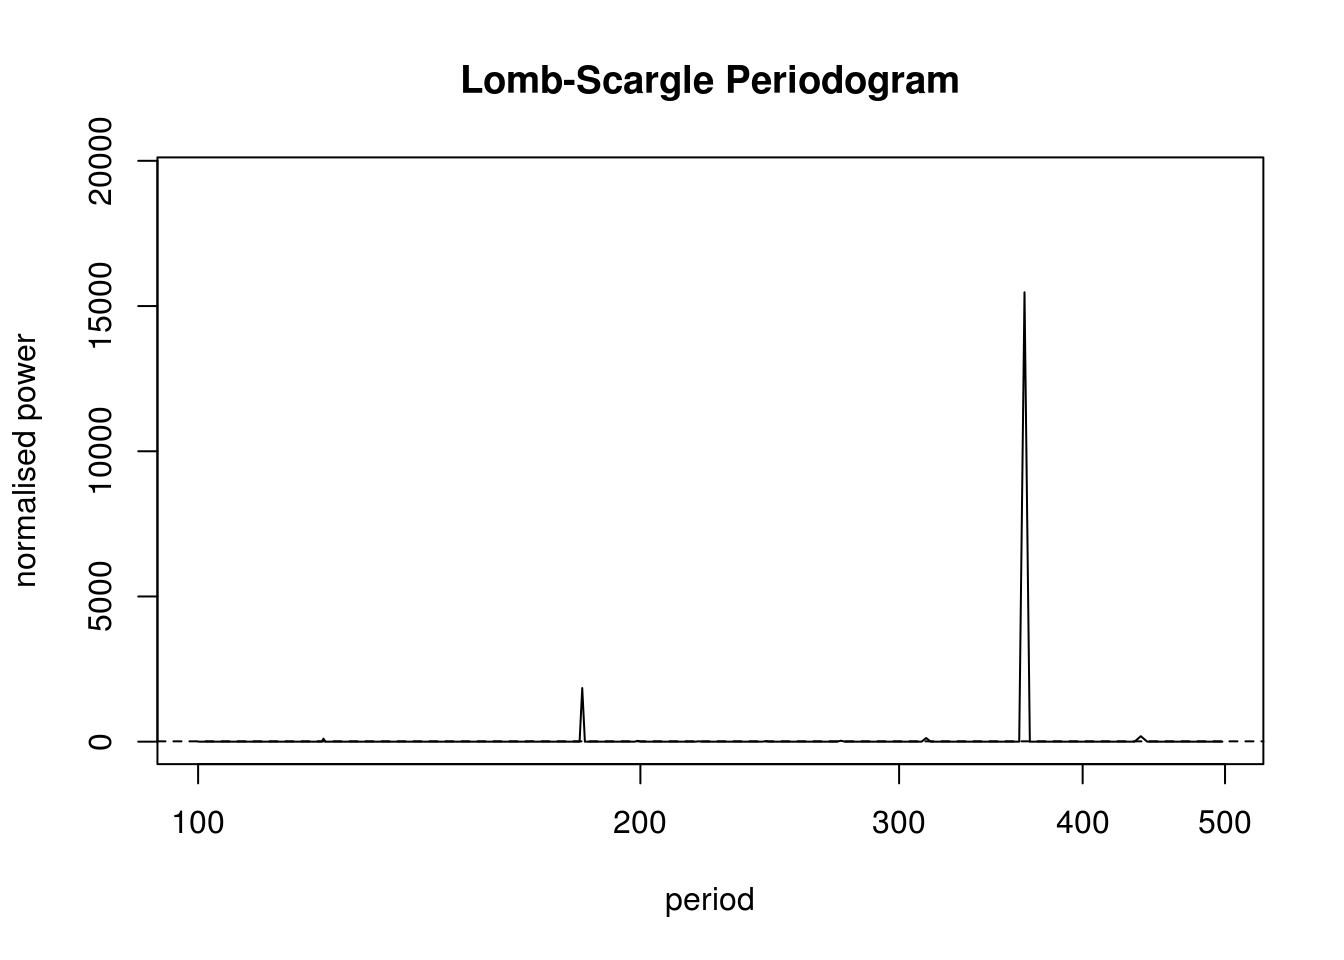
\includegraphics{website_files/figure-latex/unnamed-chunk-45-1.pdf}

\newpage

\section{Regression}\label{regression-1}

First we create an \texttt{id} variable. This generally corresponds to
geographical locations, or people. In this case, we only have one
geographical location, so our \texttt{id} for all observations is
\texttt{1}. This lets the computer know that all data belongs to the
same group.

When we have panel data with multiple areas, we use the
\texttt{MASS::glmPQL} function in R and the \texttt{meglm} function in
STATA. In R we identify the geographical areas with
\texttt{random\ =\ \textasciitilde{}\ 1\ \textbar{}\ fylke} and in STATA
with \texttt{\textbar{}\textbar{}\ fylke:}.

\begin{verbatim}
// STATA CODE STARTS
gen cos365=cos(dayofyear*2*_pi/365)
gen sin365=sin(dayofyear*2*_pi/365)

meglm y yearminus2000 || fylke:, family(poisson) iter(10)
estimates store m1
meglm y yearminus2000 cos365 sin365 || fylke:, family(poisson) iter(10)
estimates store m2

predict resid, anscombe

lrtest m1 m2
// STATA CODE ENDS
\end{verbatim}

\begin{Shaded}
\begin{Highlighting}[]
\CommentTok{# R CODE}
\NormalTok{d[,cos365}\OperatorTok{:}\ErrorTok{=}\KeywordTok{cos}\NormalTok{(dayOfYear}\OperatorTok{*}\DecValTok{2}\OperatorTok{*}\NormalTok{pi}\OperatorTok{/}\DecValTok{365}\NormalTok{)]}
\NormalTok{d[,sin365}\OperatorTok{:}\ErrorTok{=}\KeywordTok{sin}\NormalTok{(dayOfYear}\OperatorTok{*}\DecValTok{2}\OperatorTok{*}\NormalTok{pi}\OperatorTok{/}\DecValTok{365}\NormalTok{)]}
\NormalTok{fit0 <-}\StringTok{ }\NormalTok{MASS}\OperatorTok{::}\KeywordTok{glmmPQL}\NormalTok{(y}\OperatorTok{~}\NormalTok{yearMinus2000, }\DataTypeTok{random =} \OperatorTok{~}\StringTok{ }\DecValTok{1} \OperatorTok{|}\StringTok{ }\NormalTok{fylke,}
                \DataTypeTok{family =}\NormalTok{ poisson, }\DataTypeTok{data =}\NormalTok{ d)}
\end{Highlighting}
\end{Shaded}

\begin{verbatim}
## iteration 1
\end{verbatim}

\begin{Shaded}
\begin{Highlighting}[]
\NormalTok{fit1 <-}\StringTok{ }\NormalTok{MASS}\OperatorTok{::}\KeywordTok{glmmPQL}\NormalTok{(y}\OperatorTok{~}\NormalTok{yearMinus2000 }\OperatorTok{+}\StringTok{ }\NormalTok{sin365 }\OperatorTok{+}\StringTok{ }\NormalTok{cos365, }\DataTypeTok{random =} \OperatorTok{~}\StringTok{ }\DecValTok{1} \OperatorTok{|}\StringTok{ }\NormalTok{fylke,}
                \DataTypeTok{family =}\NormalTok{ poisson, }\DataTypeTok{data =}\NormalTok{ d)}
\end{Highlighting}
\end{Shaded}

\begin{verbatim}
## iteration 1
\end{verbatim}

\begin{Shaded}
\begin{Highlighting}[]
\KeywordTok{print}\NormalTok{(lmtest}\OperatorTok{::}\KeywordTok{lrtest}\NormalTok{(fit0, fit1))}
\end{Highlighting}
\end{Shaded}

\begin{verbatim}
## Likelihood ratio test
## 
## Model 1: y ~ yearMinus2000
## Model 2: y ~ yearMinus2000 + sin365 + cos365
##   #Df LogLik Df Chisq Pr(>Chisq)
## 1   4                           
## 2   6         2
\end{verbatim}

We see that the likelihood ratio test for \texttt{sin365} and
\texttt{cos365} was significant, meaning that there is significant
seasonality with a 365 day periodicity in our data (which we already
strongly suspected due to the periodogram).

\newpage

We can now run/look at the results of our main regression.

\begin{Shaded}
\begin{Highlighting}[]
\KeywordTok{print}\NormalTok{(}\KeywordTok{summary}\NormalTok{(fit1))}
\end{Highlighting}
\end{Shaded}

\begin{verbatim}
## Linear mixed-effects model fit by maximum likelihood
##  Data: d 
##   AIC BIC logLik
##    NA  NA     NA
## 
## Random effects:
##  Formula: ~1 | fylke
##          (Intercept)  Residual
## StdDev: 1.583894e-05 0.9976713
## 
## Variance function:
##  Structure: fixed weights
##  Formula: ~invwt 
## Fixed effects: y ~ yearMinus2000 + sin365 + cos365 
##                    Value   Std.Error    DF   t-value p-value
## (Intercept)    0.1122536 0.014488403 43797    7.7478       0
## yearMinus2000  0.0989047 0.001109477 43797   89.1453       0
## sin365         1.4095095 0.003695341 43797  381.4288       0
## cos365        -0.5109375 0.003083683 43797 -165.6907       0
##  Correlation: 
##               (Intr) yM2000 sin365
## yearMinus2000 -0.979              
## sin365        -0.150  0.000       
## cos365         0.065 -0.001 -0.151
## 
## Standardized Within-Group Residuals:
##         Min          Q1         Med          Q3         Max 
## -3.19682240 -0.82387498 -0.07501834  0.63400484  5.82452468 
## 
## Number of Observations: 43820
## Number of Groups: 20
\end{verbatim}

\newpage

\section{Residual analysis}\label{residual-analysis-1}

We see that there is no evidence of autoregression in the residuals

\begin{verbatim}
// STATA CODE STARTS
pac resid if fylke==1
// STATA CODE ENDS
\end{verbatim}

\begin{Shaded}
\begin{Highlighting}[]
\CommentTok{# R CODE}
\KeywordTok{pacf}\NormalTok{(}\KeywordTok{residuals}\NormalTok{(fit1, }\DataTypeTok{type =} \StringTok{"normalized"}\NormalTok{)) }\CommentTok{# this is for AR}
\end{Highlighting}
\end{Shaded}

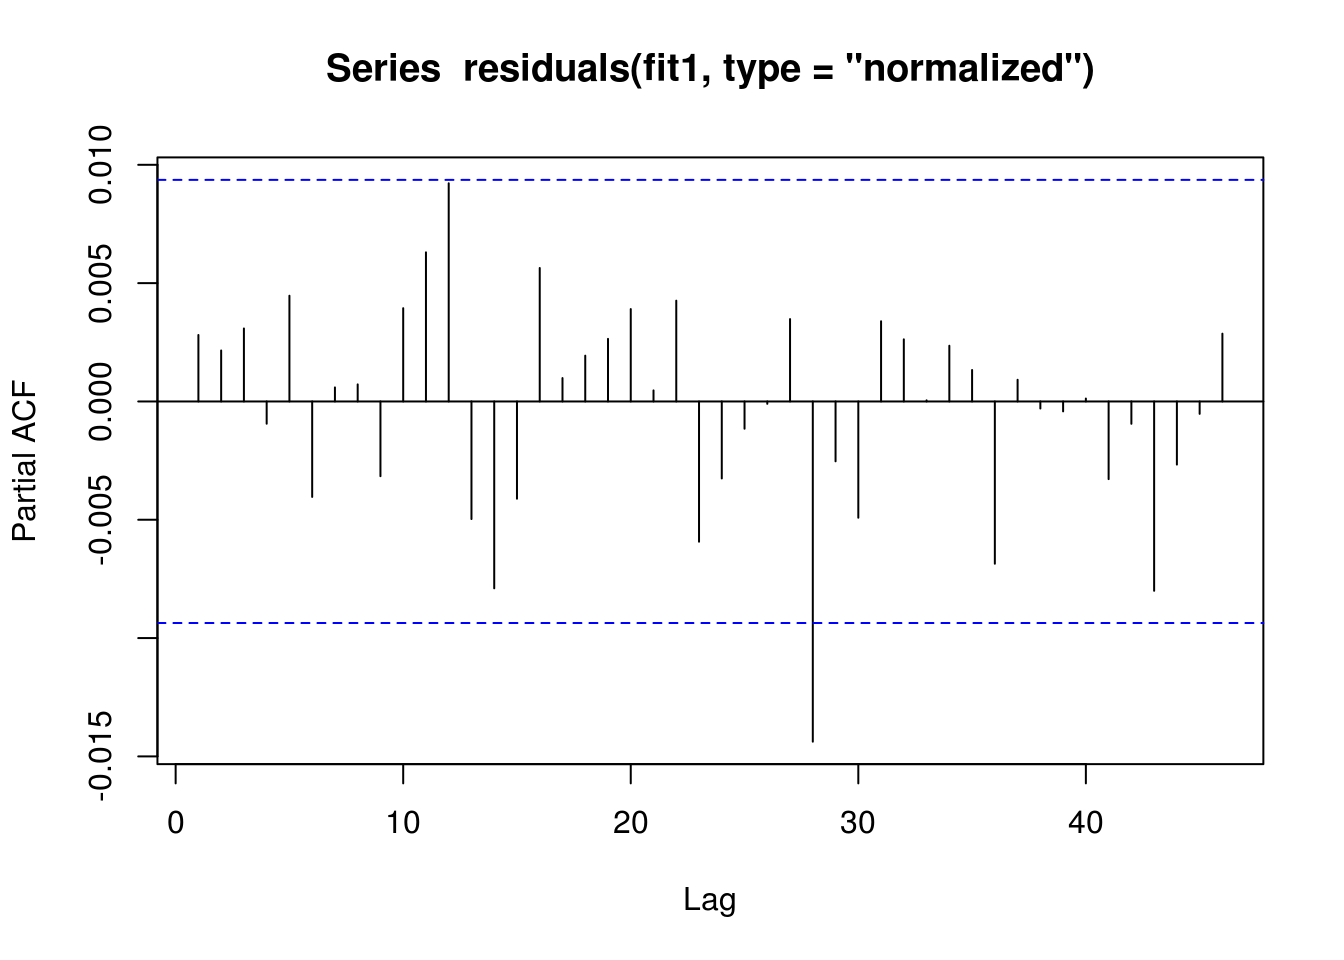
\includegraphics{website_files/figure-latex/unnamed-chunk-48-1.pdf}

\newpage

We see that there is no evidence of autoregression in the residuals

\begin{verbatim}
// STATA CODE STARTS
ac resid if fylke==1
// STATA CODE ENDS
\end{verbatim}

\begin{Shaded}
\begin{Highlighting}[]
\CommentTok{# R CODE}
\KeywordTok{acf}\NormalTok{(}\KeywordTok{residuals}\NormalTok{(fit1, }\DataTypeTok{type =} \StringTok{"normalized"}\NormalTok{)) }\CommentTok{# this is for MA}
\end{Highlighting}
\end{Shaded}

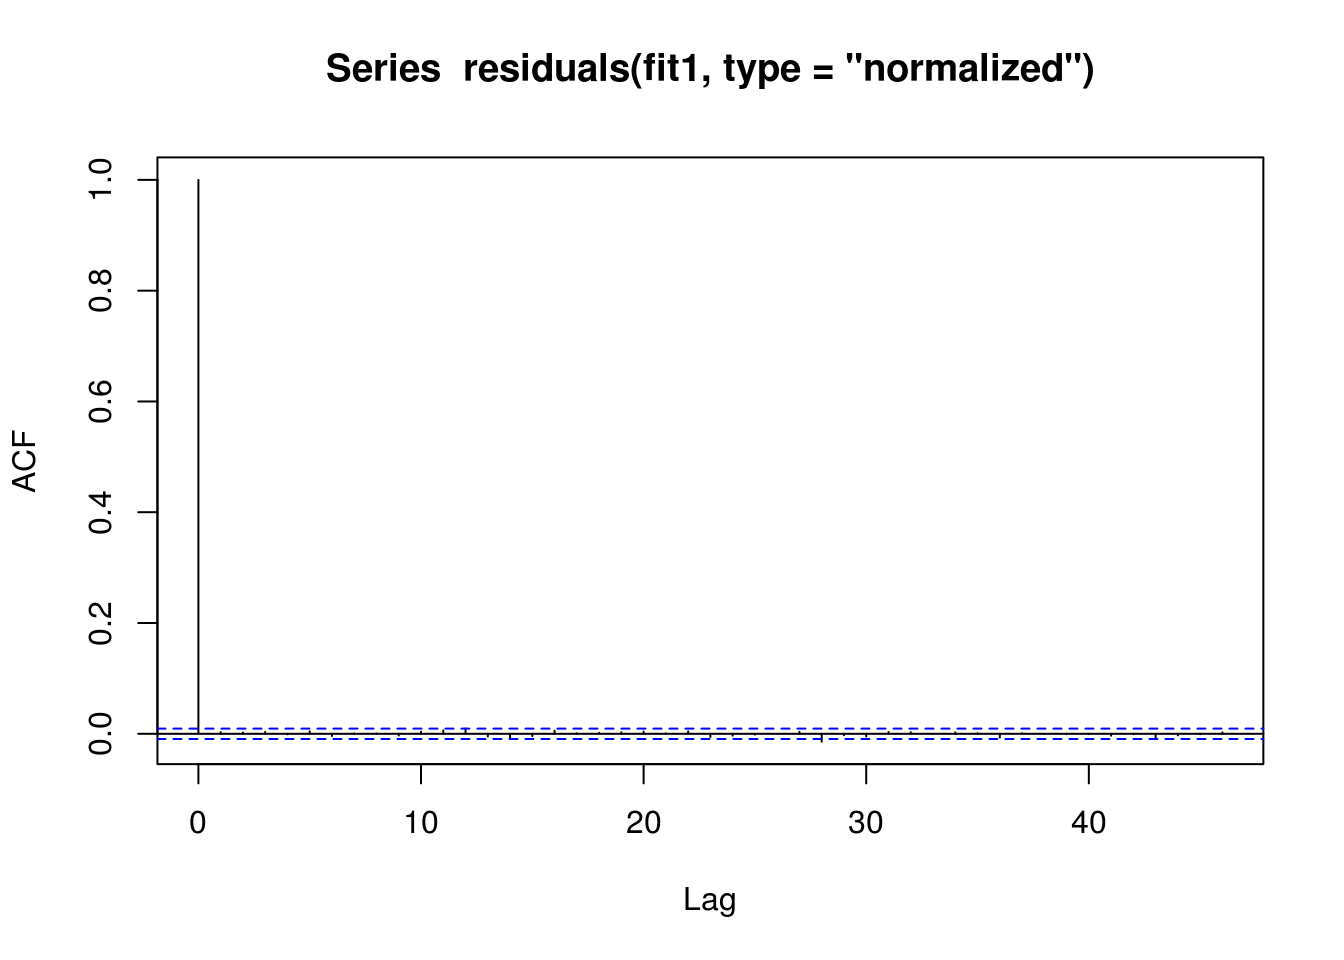
\includegraphics{website_files/figure-latex/unnamed-chunk-49-1.pdf}

\newpage

We also obtain the same estimates that we did in the last chapter.

\begin{Shaded}
\begin{Highlighting}[]
\NormalTok{b1 <-}\StringTok{ }\FloatTok{1.4007640} \CommentTok{# sin coefficient}
\NormalTok{b2 <-}\StringTok{ }\OperatorTok{-}\FloatTok{0.5234863} \CommentTok{# cos coefficient}
\NormalTok{amplitude <-}\StringTok{ }\KeywordTok{sqrt}\NormalTok{(b1}\OperatorTok{^}\DecValTok{2} \OperatorTok{+}\StringTok{ }\NormalTok{b2}\OperatorTok{^}\DecValTok{2}\NormalTok{)}
\NormalTok{p <-}\StringTok{ }\KeywordTok{atan}\NormalTok{(b1}\OperatorTok{/}\NormalTok{b2) }\OperatorTok{*}\StringTok{ }\DecValTok{365}\OperatorTok{/}\DecValTok{2}\OperatorTok{/}\NormalTok{pi}
\ControlFlowTok{if}\NormalTok{ (p }\OperatorTok{>}\StringTok{ }\DecValTok{0}\NormalTok{) \{}
\NormalTok{    peak <-}\StringTok{ }\NormalTok{p}
\NormalTok{    trough <-}\StringTok{ }\NormalTok{p }\OperatorTok{+}\StringTok{ }\DecValTok{365}\OperatorTok{/}\DecValTok{2}
\NormalTok{\} }\ControlFlowTok{else}\NormalTok{ \{}
\NormalTok{    peak <-}\StringTok{ }\NormalTok{p }\OperatorTok{+}\StringTok{ }\DecValTok{365}\OperatorTok{/}\DecValTok{2}
\NormalTok{    trough <-}\StringTok{ }\NormalTok{p }\OperatorTok{+}\StringTok{ }\DecValTok{365}
\NormalTok{\}}
\ControlFlowTok{if}\NormalTok{ (b1 }\OperatorTok{<}\StringTok{ }\DecValTok{0}\NormalTok{) \{}
\NormalTok{    g <-}\StringTok{ }\NormalTok{peak}
\NormalTok{    peak <-}\StringTok{ }\NormalTok{trough}
\NormalTok{    trough <-}\StringTok{ }\NormalTok{g}
\NormalTok{\}}
\KeywordTok{print}\NormalTok{(}\KeywordTok{sprintf}\NormalTok{(}\StringTok{"amplitude is estimated as %s, peak is estimated as %s, trough is estimated as %s"}\NormalTok{,}\KeywordTok{round}\NormalTok{(amplitude,}\DecValTok{2}\NormalTok{),}\KeywordTok{round}\NormalTok{(peak),}\KeywordTok{round}\NormalTok{(trough)))}
\end{Highlighting}
\end{Shaded}

\begin{verbatim}
## [1] "amplitude is estimated as 1.5, peak is estimated as 112, trough is estimated as 295"
\end{verbatim}

\begin{Shaded}
\begin{Highlighting}[]
\KeywordTok{print}\NormalTok{(}\KeywordTok{sprintf}\NormalTok{(}\StringTok{"true values are: amplitude: %s, peak: %s, trough: %s"}\NormalTok{,}\KeywordTok{round}\NormalTok{(AMPLITUDE,}\DecValTok{2}\NormalTok{),}\KeywordTok{round}\NormalTok{(}\DecValTok{365}\OperatorTok{/}\DecValTok{4}\OperatorTok{+}\NormalTok{SEASONAL_HORIZONTAL_SHIFT),}\KeywordTok{round}\NormalTok{(}\DecValTok{3}\OperatorTok{*}\DecValTok{365}\OperatorTok{/}\DecValTok{4}\OperatorTok{+}\NormalTok{SEASONAL_HORIZONTAL_SHIFT)))}
\end{Highlighting}
\end{Shaded}

\begin{verbatim}
## [1] "true values are: amplitude: 1.5, peak: 111, trough: 294"
\end{verbatim}

\chapter{Panel data: multiple areas with
autocorrelation}\label{panel-data-multiple-areas-with-autocorrelation}

\section{Aim}\label{aim-4}

We are given a dataset containing daily counts of diseases from multiple
geographical areas. We want to identify:

\begin{itemize}
\tightlist
\item
  Does seasonality exist?
\item
  If seasonality exists, when are the high/low seasons?
\item
  Is there a general yearly trend (i.e.~increasing or decreasing from
  year to year?)
\end{itemize}

\newpage

\section{Creating the data}\label{creating-the-data-4}

The data for this chapter is available at:
\url{http://rwhite.no/longitudinal_analysis/data/chapter_7.csv}

\begin{Shaded}
\begin{Highlighting}[]
\KeywordTok{library}\NormalTok{(data.table)}
\KeywordTok{library}\NormalTok{(ggplot2)}
\KeywordTok{set.seed}\NormalTok{(}\DecValTok{4}\NormalTok{)}

\NormalTok{AMPLITUDE <-}\StringTok{ }\FloatTok{1.5}
\NormalTok{SEASONAL_HORIZONTAL_SHIFT <-}\StringTok{ }\DecValTok{20}

\NormalTok{fylkeIntercepts <-}\StringTok{ }\KeywordTok{data.table}\NormalTok{(}\DataTypeTok{fylke=}\DecValTok{1}\OperatorTok{:}\DecValTok{20}\NormalTok{,}\DataTypeTok{fylkeIntercepts=}\KeywordTok{rnorm}\NormalTok{(}\DecValTok{20}\NormalTok{))}

\NormalTok{d <-}\StringTok{ }\KeywordTok{data.table}\NormalTok{(}\DataTypeTok{date=}\KeywordTok{seq.Date}\NormalTok{(}
  \DataTypeTok{from=}\KeywordTok{as.Date}\NormalTok{(}\StringTok{"2010-01-01"}\NormalTok{),}
  \DataTypeTok{to=}\KeywordTok{as.Date}\NormalTok{(}\StringTok{"2015-12-31"}\NormalTok{),}
  \DataTypeTok{by=}\DecValTok{1}\NormalTok{))}
\NormalTok{d[,year}\OperatorTok{:}\ErrorTok{=}\KeywordTok{as.numeric}\NormalTok{(}\KeywordTok{format.Date}\NormalTok{(date,}\StringTok{"%G"}\NormalTok{))]}
\NormalTok{d[,week}\OperatorTok{:}\ErrorTok{=}\KeywordTok{as.numeric}\NormalTok{(}\KeywordTok{format.Date}\NormalTok{(date,}\StringTok{"%V"}\NormalTok{))]}
\NormalTok{d[,month}\OperatorTok{:}\ErrorTok{=}\KeywordTok{as.numeric}\NormalTok{(}\KeywordTok{format.Date}\NormalTok{(date,}\StringTok{"%m"}\NormalTok{))]}

\NormalTok{temp <-}\StringTok{ }\KeywordTok{vector}\NormalTok{(}\StringTok{"list"}\NormalTok{,}\DataTypeTok{length=}\DecValTok{20}\NormalTok{)}
\ControlFlowTok{for}\NormalTok{(i }\ControlFlowTok{in} \DecValTok{1}\OperatorTok{:}\DecValTok{20}\NormalTok{)\{}
\NormalTok{  temp[[i]] <-}\StringTok{ }\KeywordTok{copy}\NormalTok{(d)}
\NormalTok{  temp[[i]][,fylke}\OperatorTok{:}\ErrorTok{=}\NormalTok{i]}
\NormalTok{\}}
\NormalTok{d <-}\StringTok{ }\KeywordTok{rbindlist}\NormalTok{(temp)}

\NormalTok{d[,yearMinus2000}\OperatorTok{:}\ErrorTok{=}\NormalTok{year}\OperatorTok{-}\DecValTok{2000}\NormalTok{]}
\NormalTok{d[,dayOfSeries}\OperatorTok{:}\ErrorTok{=}\DecValTok{1}\OperatorTok{:}\NormalTok{.N]}

\NormalTok{d[,dayOfYear}\OperatorTok{:}\ErrorTok{=}\KeywordTok{as.numeric}\NormalTok{(}\KeywordTok{format.Date}\NormalTok{(date,}\StringTok{"%j"}\NormalTok{))]}
\NormalTok{d[,seasonalEffect}\OperatorTok{:}\ErrorTok{=}\KeywordTok{sin}\NormalTok{(}\DecValTok{2}\OperatorTok{*}\NormalTok{pi}\OperatorTok{*}\NormalTok{(dayOfYear}\OperatorTok{-}\NormalTok{SEASONAL_HORIZONTAL_SHIFT)}\OperatorTok{/}\DecValTok{365}\NormalTok{)]}
\NormalTok{d[,mu }\OperatorTok{:}\ErrorTok{=}\StringTok{ }\KeywordTok{round}\NormalTok{(}\KeywordTok{exp}\NormalTok{(}\FloatTok{0.1} \OperatorTok{+}\StringTok{ }\NormalTok{yearMinus2000}\OperatorTok{*}\FloatTok{0.1} \OperatorTok{+}\StringTok{ }\NormalTok{seasonalEffect}\OperatorTok{*}\NormalTok{AMPLITUDE))]}
\NormalTok{d[,y}\OperatorTok{:}\ErrorTok{=}\KeywordTok{rpois}\NormalTok{(.N,mu)]}
\NormalTok{d[,y}\OperatorTok{:}\ErrorTok{=}\NormalTok{mu}\OperatorTok{+}\KeywordTok{round}\NormalTok{(}\KeywordTok{as.numeric}\NormalTok{(}\KeywordTok{arima.sim}\NormalTok{(}\DataTypeTok{model=}\KeywordTok{list}\NormalTok{(}\StringTok{"ar"}\NormalTok{=}\KeywordTok{c}\NormalTok{(}\FloatTok{0.5}\NormalTok{)), }\DataTypeTok{rand.gen =}\NormalTok{ rpois, }\DataTypeTok{n=}\KeywordTok{nrow}\NormalTok{(d), }\DataTypeTok{lambda=}\NormalTok{mu)))]}

\KeywordTok{fwrite}\NormalTok{(d,}\StringTok{"data/chapter_7.csv"}\NormalTok{)}
\end{Highlighting}
\end{Shaded}

\newpage

\section{Investigation}\label{investigation-3}

We drill down into a few years in fylke 1, and see a clear seasonal
trend

\begin{Shaded}
\begin{Highlighting}[]
\NormalTok{q <-}\StringTok{ }\KeywordTok{ggplot}\NormalTok{(d[fylke}\OperatorTok{==}\DecValTok{1}\NormalTok{],}\KeywordTok{aes}\NormalTok{(}\DataTypeTok{x=}\NormalTok{dayOfYear,}\DataTypeTok{y=}\NormalTok{y))}
\NormalTok{q <-}\StringTok{ }\NormalTok{q }\OperatorTok{+}\StringTok{ }\KeywordTok{facet_wrap}\NormalTok{(}\OperatorTok{~}\NormalTok{year)}
\NormalTok{q <-}\StringTok{ }\NormalTok{q }\OperatorTok{+}\StringTok{ }\KeywordTok{geom_point}\NormalTok{()}
\NormalTok{q <-}\StringTok{ }\NormalTok{q }\OperatorTok{+}\StringTok{ }\KeywordTok{stat_smooth}\NormalTok{(}\DataTypeTok{colour=}\StringTok{"red"}\NormalTok{)}
\NormalTok{q}
\end{Highlighting}
\end{Shaded}

\begin{verbatim}
## `geom_smooth()` using method = 'loess' and formula 'y ~ x'
\end{verbatim}

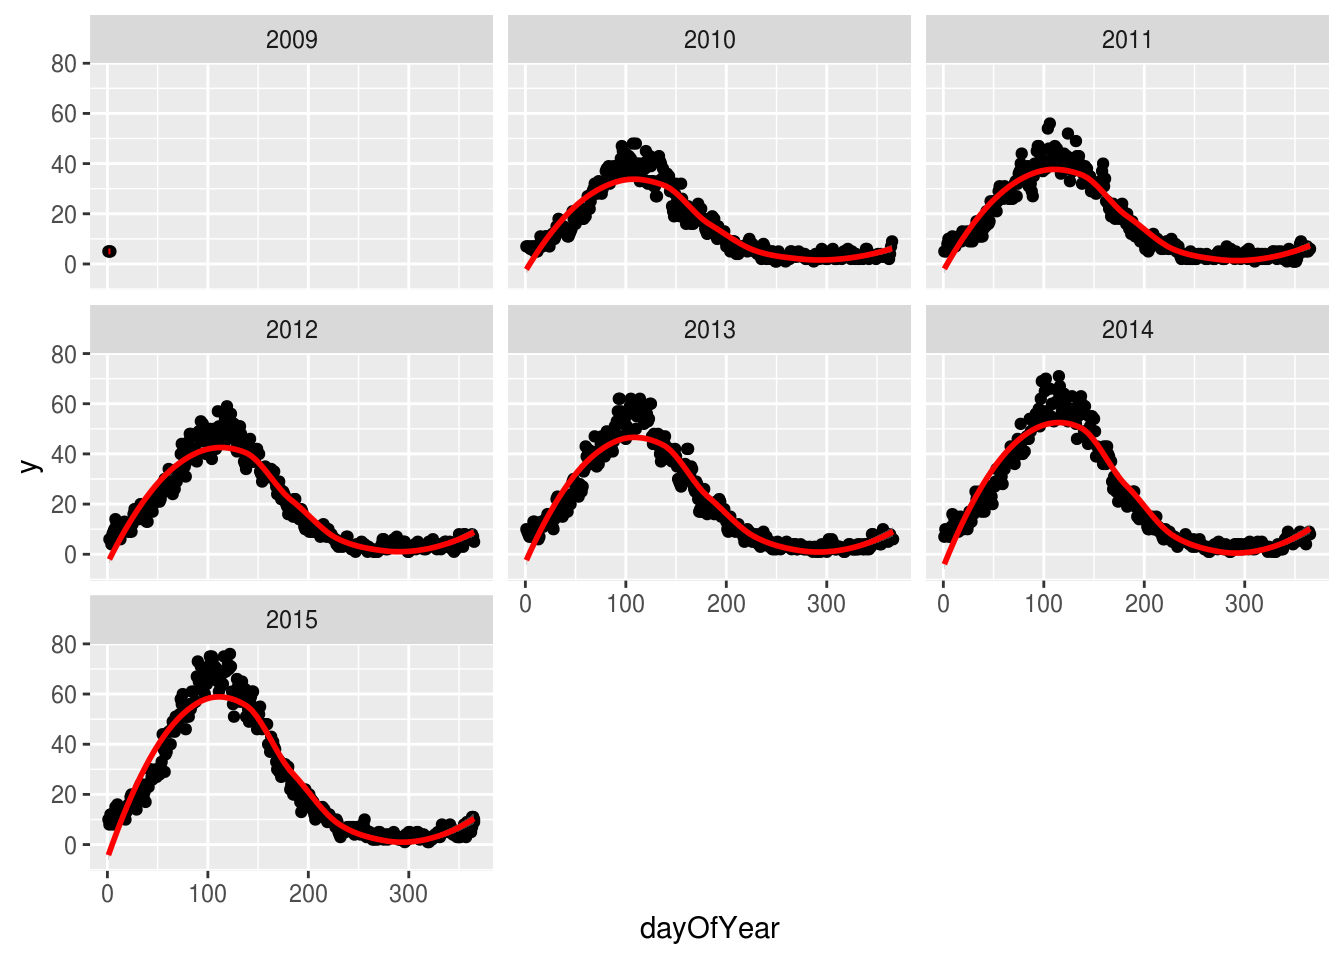
\includegraphics{website_files/figure-latex/unnamed-chunk-52-1.pdf}

\newpage

The Lomb-Scargle Periodogram shows a clear seasonality with a period of
365 days

\begin{verbatim}
// STATA CODE STARTS
insheet using "chapter_7.csv", clear

sort fylke date
by fylke: gen time=_n
tsset fylke time, daily

wntestb y if fylke==1

cumsp y if fylke==1, gen(cumulative_spec_dist)
by fylke: gen period=_N/_n

browse cumulative_spec_dist period
// STATA CODE ENDS
\end{verbatim}

\begin{Shaded}
\begin{Highlighting}[]
\CommentTok{# R CODE}
\NormalTok{lomb}\OperatorTok{::}\KeywordTok{lsp}\NormalTok{(d}\OperatorTok{$}\NormalTok{y,}\DataTypeTok{from=}\DecValTok{100}\NormalTok{,}\DataTypeTok{to=}\DecValTok{500}\NormalTok{,}\DataTypeTok{ofac=}\DecValTok{1}\NormalTok{,}\DataTypeTok{type=}\StringTok{"period"}\NormalTok{)}
\end{Highlighting}
\end{Shaded}

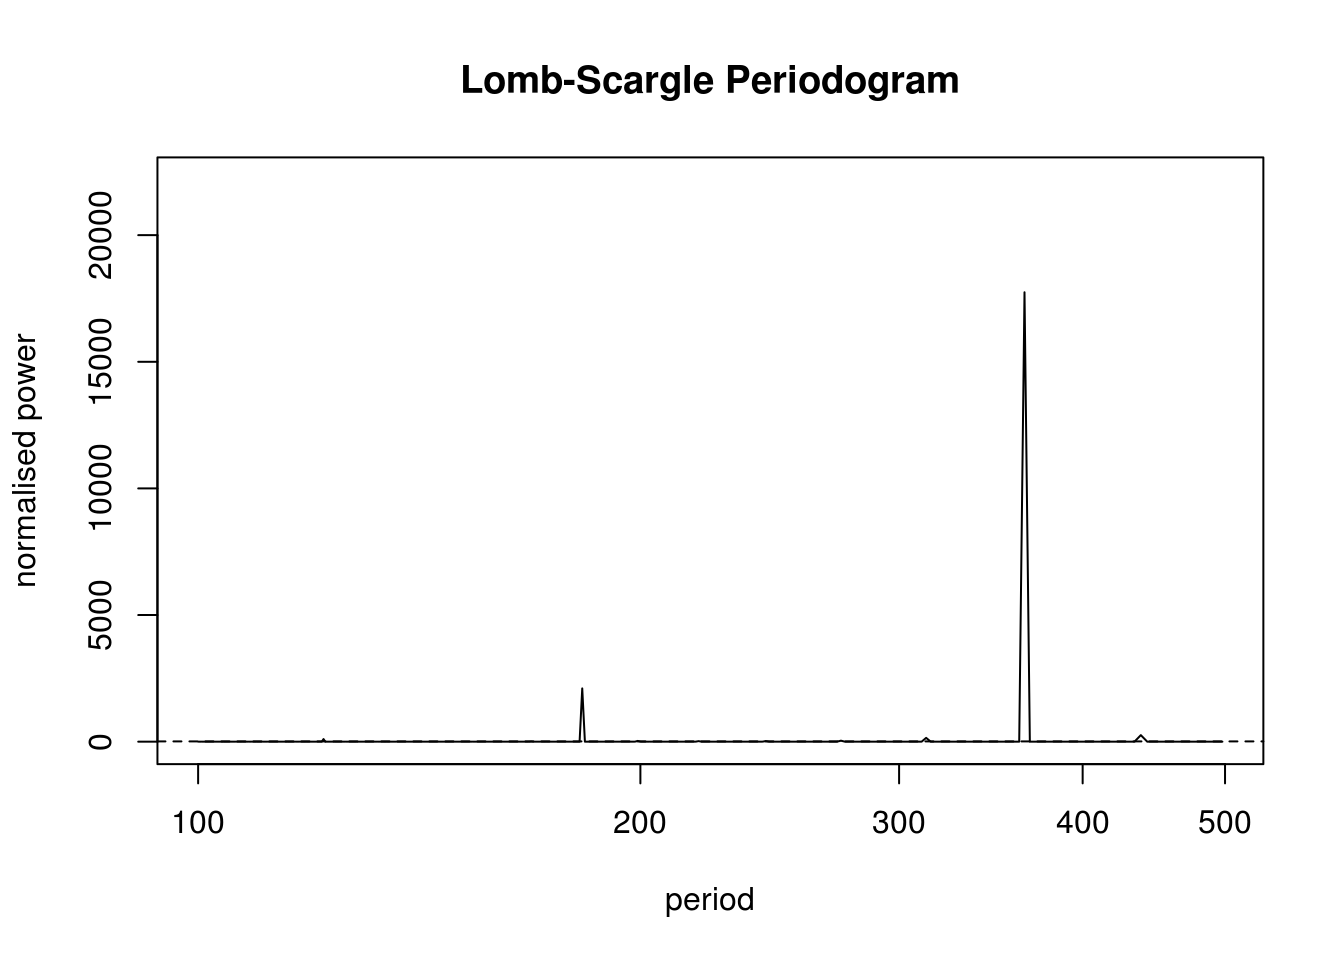
\includegraphics{website_files/figure-latex/unnamed-chunk-53-1.pdf}

\newpage

\section{Regressions}\label{regressions-1}

First we create an \texttt{id} variable. This generally corresponds to
geographical locations, or people. In this case, we only have one
geographical location, so our \texttt{id} for all observations is
\texttt{1}. This lets the computer know that all data belongs to the
same group.

When we have panel data with multiple areas, we use the
\texttt{MASS::glmPQL} function in R and the \texttt{meglm} function in
STATA. In R we identify the geographical areas with
\texttt{random\ =\ \textasciitilde{}\ §\ \textbar{}\ fylke} and in STATA
with \texttt{\textbar{}\textbar{}\ fylke:}.

\begin{verbatim}
// STATA CODE STARTS
gen cos365=cos(dayofyear*2*_pi/365)
gen sin365=sin(dayofyear*2*_pi/365)

meglm y yearminus2000 || fylke:, family(poisson) iter(10)
estimates store m1
meglm y yearminus2000 cos365 sin365 || fylke:, family(poisson) iter(10)
estimates store m2

predict resid, anscombe

lrtest m1 m2
// STATA CODE ENDS
\end{verbatim}

\begin{Shaded}
\begin{Highlighting}[]
\CommentTok{# R CODE}
\NormalTok{d[,cos365}\OperatorTok{:}\ErrorTok{=}\KeywordTok{cos}\NormalTok{(dayOfYear}\OperatorTok{*}\DecValTok{2}\OperatorTok{*}\NormalTok{pi}\OperatorTok{/}\DecValTok{365}\NormalTok{)]}
\NormalTok{d[,sin365}\OperatorTok{:}\ErrorTok{=}\KeywordTok{sin}\NormalTok{(dayOfYear}\OperatorTok{*}\DecValTok{2}\OperatorTok{*}\NormalTok{pi}\OperatorTok{/}\DecValTok{365}\NormalTok{)]}
\NormalTok{fit0 <-}\StringTok{ }\NormalTok{MASS}\OperatorTok{::}\KeywordTok{glmmPQL}\NormalTok{(y}\OperatorTok{~}\NormalTok{yearMinus2000, }\DataTypeTok{random =} \OperatorTok{~}\StringTok{ }\DecValTok{1} \OperatorTok{|}\StringTok{ }\NormalTok{fylke,}
                \DataTypeTok{family =}\NormalTok{ poisson, }\DataTypeTok{data =}\NormalTok{ d)}
\end{Highlighting}
\end{Shaded}

\begin{verbatim}
## iteration 1
\end{verbatim}

\begin{Shaded}
\begin{Highlighting}[]
\NormalTok{fit1 <-}\StringTok{ }\NormalTok{MASS}\OperatorTok{::}\KeywordTok{glmmPQL}\NormalTok{(y}\OperatorTok{~}\NormalTok{yearMinus2000 }\OperatorTok{+}\StringTok{ }\NormalTok{sin365 }\OperatorTok{+}\StringTok{ }\NormalTok{cos365, }\DataTypeTok{random =} \OperatorTok{~}\StringTok{ }\DecValTok{1} \OperatorTok{|}\StringTok{ }\NormalTok{fylke,}
                \DataTypeTok{family =}\NormalTok{ poisson, }\DataTypeTok{data =}\NormalTok{ d)}
\end{Highlighting}
\end{Shaded}

\begin{verbatim}
## iteration 1
\end{verbatim}

\begin{verbatim}
## iteration 2
\end{verbatim}

\begin{Shaded}
\begin{Highlighting}[]
\KeywordTok{print}\NormalTok{(lmtest}\OperatorTok{::}\KeywordTok{lrtest}\NormalTok{(fit0, fit1))}
\end{Highlighting}
\end{Shaded}

\begin{verbatim}
## Likelihood ratio test
## 
## Model 1: y ~ yearMinus2000
## Model 2: y ~ yearMinus2000 + sin365 + cos365
##   #Df LogLik Df Chisq Pr(>Chisq)
## 1   4                           
## 2   6         2
\end{verbatim}

We see that the likelihood ratio test for \texttt{sin365} and
\texttt{cos365} was significant, meaning that there is significant
seasonality with a 365 day periodicity in our data (which we already
strongly suspected due to the periodogram).

\newpage

We can now run/look at the results of our main regression.

\begin{Shaded}
\begin{Highlighting}[]
\KeywordTok{print}\NormalTok{(}\KeywordTok{summary}\NormalTok{(fit1))}
\end{Highlighting}
\end{Shaded}

\begin{verbatim}
## Linear mixed-effects model fit by maximum likelihood
##  Data: d 
##   AIC BIC logLik
##    NA  NA     NA
## 
## Random effects:
##  Formula: ~1 | fylke
##         (Intercept)  Residual
## StdDev: 0.004579768 0.7191519
## 
## Variance function:
##  Structure: fixed weights
##  Formula: ~invwt 
## Fixed effects: y ~ yearMinus2000 + sin365 + cos365 
##                    Value   Std.Error    DF   t-value p-value
## (Intercept)    1.2189925 0.006110555 43797  199.4896       0
## yearMinus2000  0.0987374 0.000461394 43797  213.9980       0
## sin365         1.3990267 0.001531179 43797  913.6928       0
## cos365        -0.5171211 0.001282191 43797 -403.3106       0
##  Correlation: 
##               (Intr) yM2000 sin365
## yearMinus2000 -0.966              
## sin365        -0.147  0.000       
## cos365         0.065 -0.001 -0.152
## 
## Standardized Within-Group Residuals:
##         Min          Q1         Med          Q3         Max 
## -3.00864057 -0.70228031 -0.06334676  0.64274011  5.21710224 
## 
## Number of Observations: 43820
## Number of Groups: 20
\end{verbatim}

\newpage

\section{Residual analysis}\label{residual-analysis-2}

We see that there is an \texttt{AR(1)} autocorrelation in the residuals,
meaning that our model is not appropriate.

\begin{verbatim}
// STATA CODE STARTS
pac resid if fylke==1
// STATA CODE ENDS
\end{verbatim}

\begin{Shaded}
\begin{Highlighting}[]
\CommentTok{# R CODE}
\KeywordTok{pacf}\NormalTok{(}\KeywordTok{residuals}\NormalTok{(fit1, }\DataTypeTok{type =} \StringTok{"normalized"}\NormalTok{)) }\CommentTok{# this is for AR}
\end{Highlighting}
\end{Shaded}

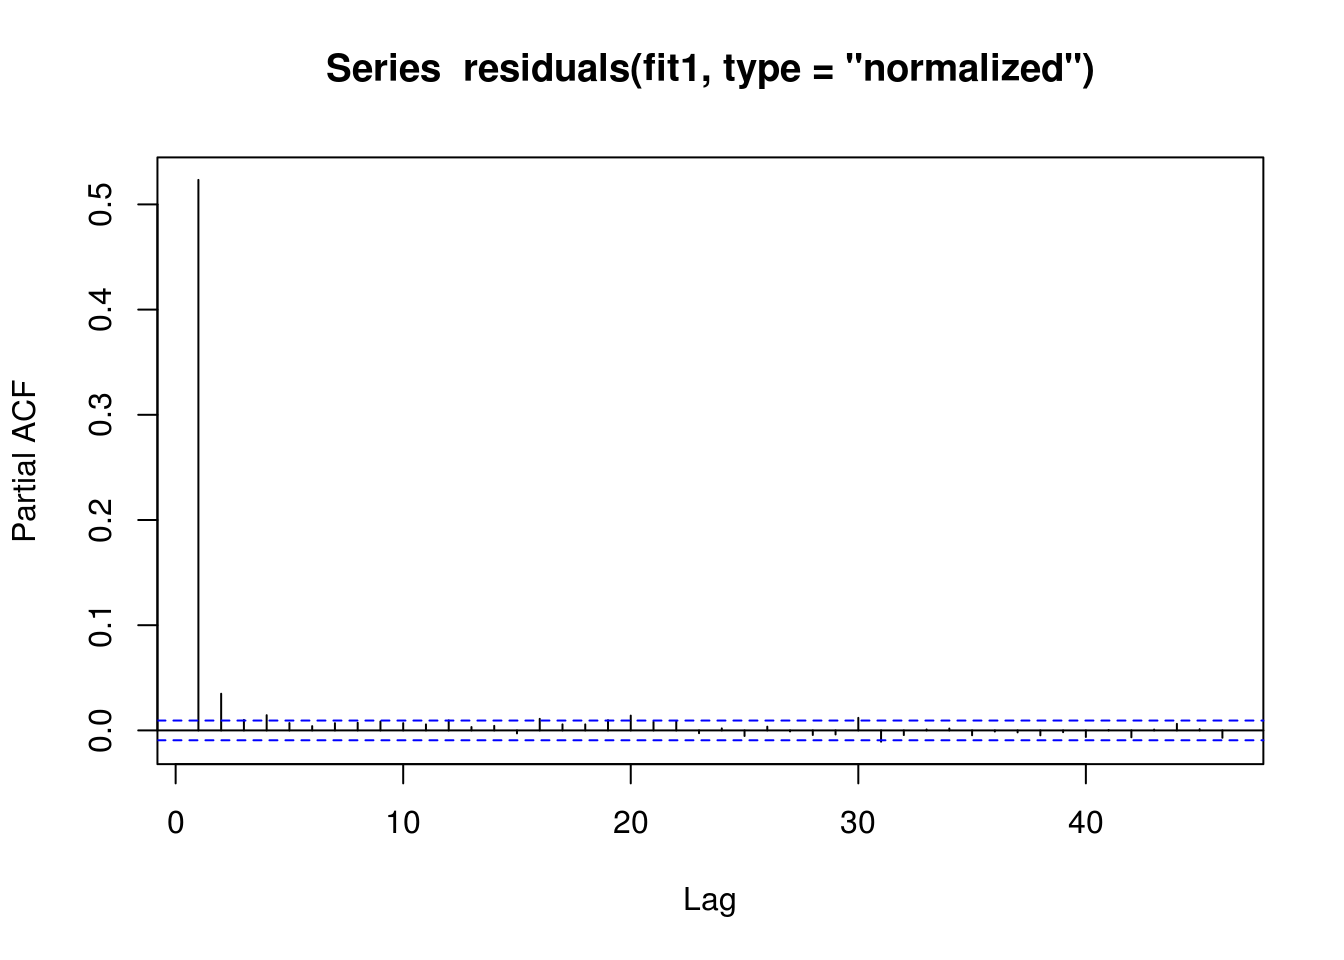
\includegraphics{website_files/figure-latex/unnamed-chunk-56-1.pdf}

\newpage

We see that there is some sort of \texttt{AR} autocorrelation in the
residuals, meaning that our model is not appropriate.

\begin{verbatim}
// STATA CODE STARTS
ac resid if fylke==1
// STATA CODE ENDS
\end{verbatim}

\begin{Shaded}
\begin{Highlighting}[]
\CommentTok{# R CODE}
\KeywordTok{acf}\NormalTok{(}\KeywordTok{residuals}\NormalTok{(fit1, }\DataTypeTok{type =} \StringTok{"normalized"}\NormalTok{)) }\CommentTok{# this is for MA}
\end{Highlighting}
\end{Shaded}

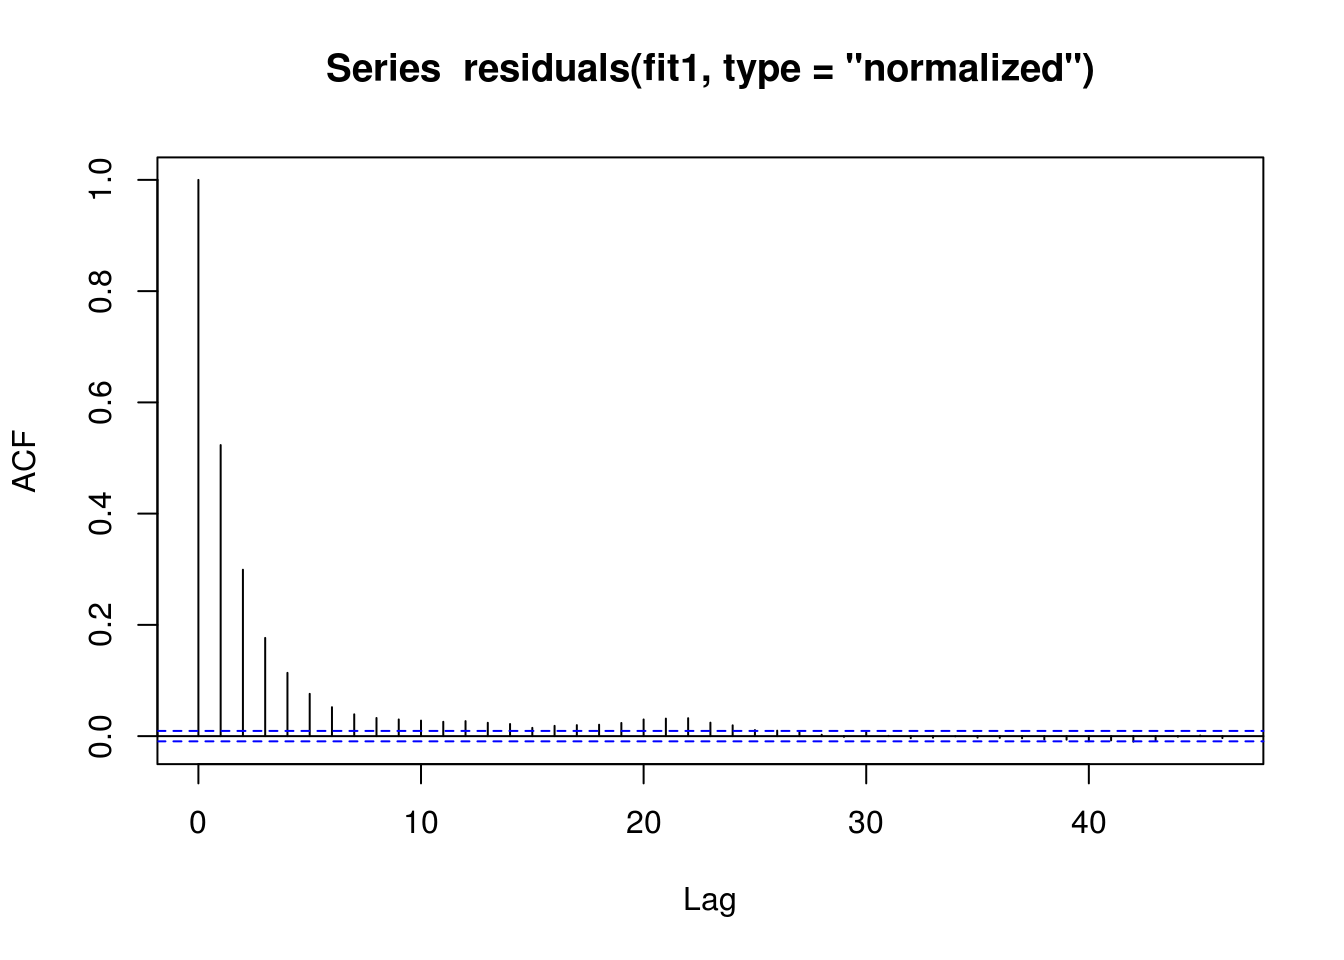
\includegraphics{website_files/figure-latex/unnamed-chunk-57-1.pdf}

\newpage

\section{(R ONLY) Regression with AR(1) correlation in
residuals}\label{r-only-regression-with-ar1-correlation-in-residuals-1}

We include
\texttt{correlation=nlme::corAR1(form=\textasciitilde{}dayOfSeries\textbar{}fylke)}
or in other words
\texttt{correlation=nlme::corAR1(form=\textasciitilde{}time\textbar{}group)}
to let the computer know what is the time variable and what is the group
variable.

\begin{Shaded}
\begin{Highlighting}[]
\NormalTok{fit1 <-}\StringTok{ }\NormalTok{MASS}\OperatorTok{::}\KeywordTok{glmmPQL}\NormalTok{(y}\OperatorTok{~}\NormalTok{yearMinus2000}\OperatorTok{+}\NormalTok{sin365 }\OperatorTok{+}\StringTok{ }\NormalTok{cos365, }\DataTypeTok{random =} \OperatorTok{~}\StringTok{ }\DecValTok{1} \OperatorTok{|}\StringTok{ }\NormalTok{fylke,}
                \DataTypeTok{family =}\NormalTok{ poisson, }\DataTypeTok{data =}\NormalTok{ d,}
                \DataTypeTok{correlation=}\NormalTok{nlme}\OperatorTok{::}\KeywordTok{corAR1}\NormalTok{(}\DataTypeTok{form=}\OperatorTok{~}\NormalTok{dayOfSeries}\OperatorTok{|}\NormalTok{fylke))}
\end{Highlighting}
\end{Shaded}

\begin{verbatim}
## iteration 1
\end{verbatim}

\begin{Shaded}
\begin{Highlighting}[]
\KeywordTok{summary}\NormalTok{(fit1)}
\end{Highlighting}
\end{Shaded}

\begin{verbatim}
## Linear mixed-effects model fit by maximum likelihood
##  Data: d 
##   AIC BIC logLik
##    NA  NA     NA
## 
## Random effects:
##  Formula: ~1 | fylke
##         (Intercept)  Residual
## StdDev: 2.40488e-05 0.7195239
## 
## Correlation Structure: AR(1)
##  Formula: ~dayOfSeries | fylke 
##  Parameter estimate(s):
##       Phi 
## 0.5240054 
## Variance function:
##  Structure: fixed weights
##  Formula: ~invwt 
## Fixed effects: y ~ yearMinus2000 + sin365 + cos365 
##                    Value   Std.Error    DF   t-value p-value
## (Intercept)    1.2195477 0.010774796 43797  113.1852       0
## yearMinus2000  0.0987065 0.000825226 43797  119.6115       0
## sin365         1.3988945 0.002739109 43797  510.7116       0
## cos365        -0.5169579 0.002292465 43797 -225.5030       0
##  Correlation: 
##               (Intr) yM2000 sin365
## yearMinus2000 -0.979              
## sin365        -0.149  0.001       
## cos365         0.066 -0.001 -0.151
## 
## Standardized Within-Group Residuals:
##         Min          Q1         Med          Q3         Max 
## -2.99731654 -0.70249782 -0.06736726  0.64264790  5.20296607 
## 
## Number of Observations: 43820
## Number of Groups: 20
\end{verbatim}

\newpage

\section{Residual analysis}\label{residual-analysis-3}

We see that the vast majority of the autoregression in the residuals has
been removed.

\begin{Shaded}
\begin{Highlighting}[]
\KeywordTok{pacf}\NormalTok{(}\KeywordTok{residuals}\NormalTok{(fit1, }\DataTypeTok{type =} \StringTok{"normalized"}\NormalTok{)) }\CommentTok{# this is for AR}
\end{Highlighting}
\end{Shaded}

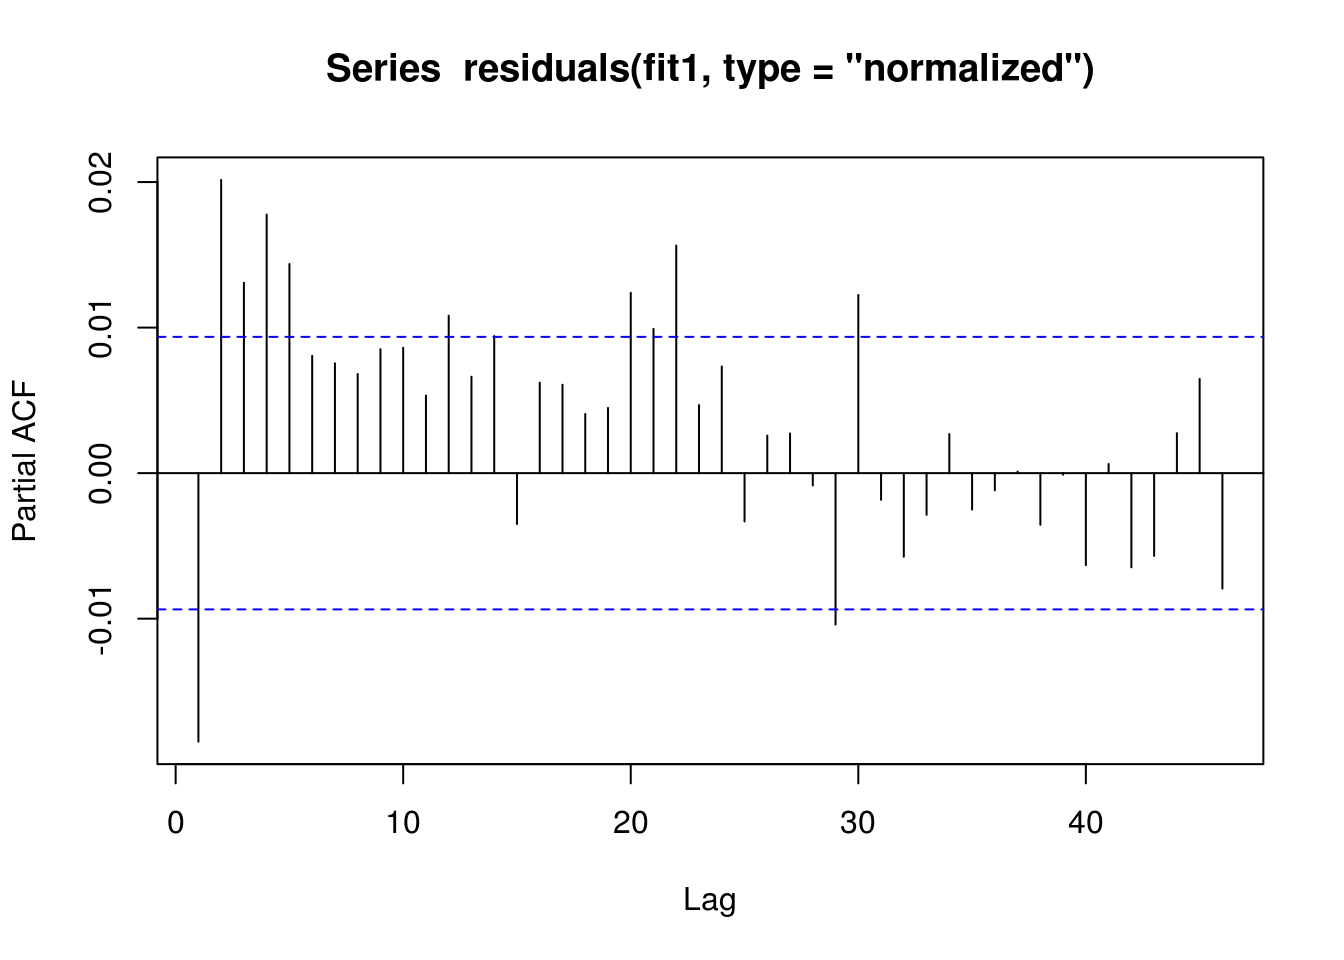
\includegraphics{website_files/figure-latex/unnamed-chunk-59-1.pdf}

\newpage

We see that the vast majority of the autoregression in the residuals has
been removed.

\begin{Shaded}
\begin{Highlighting}[]
\KeywordTok{acf}\NormalTok{(}\KeywordTok{residuals}\NormalTok{(fit1, }\DataTypeTok{type =} \StringTok{"normalized"}\NormalTok{)) }\CommentTok{# this is for MA}
\end{Highlighting}
\end{Shaded}

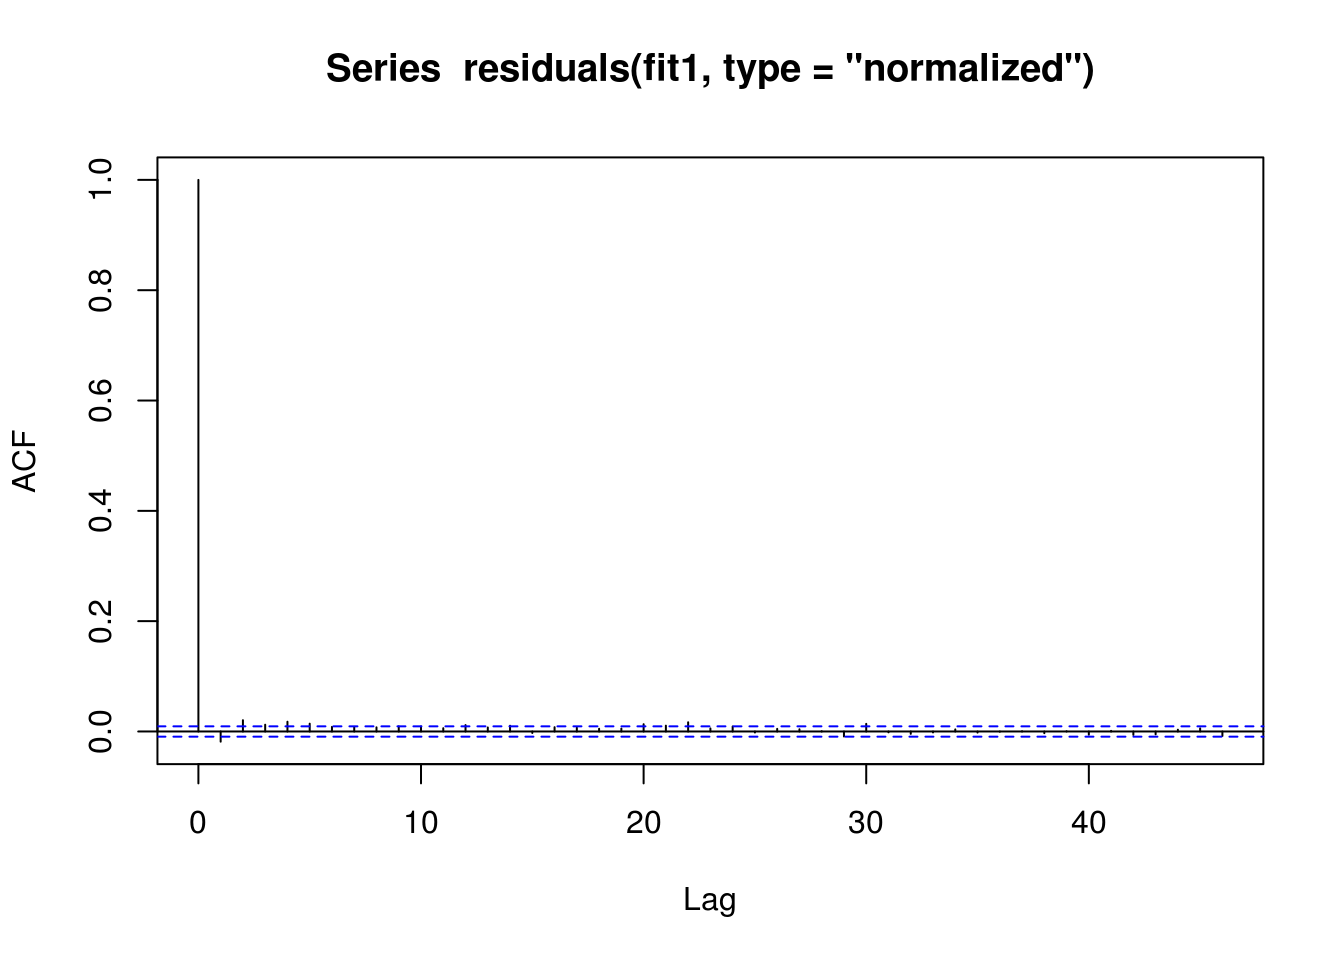
\includegraphics{website_files/figure-latex/unnamed-chunk-60-1.pdf}

\newpage

We obtain the same estimates that we did in the last chapter.

\begin{Shaded}
\begin{Highlighting}[]
\NormalTok{b1 <-}\StringTok{ }\FloatTok{1.4007640} \CommentTok{# sin coefficient}
\NormalTok{b2 <-}\StringTok{ }\OperatorTok{-}\FloatTok{0.5234863} \CommentTok{# cos coefficient}
\NormalTok{amplitude <-}\StringTok{ }\KeywordTok{sqrt}\NormalTok{(b1}\OperatorTok{^}\DecValTok{2} \OperatorTok{+}\StringTok{ }\NormalTok{b2}\OperatorTok{^}\DecValTok{2}\NormalTok{)}
\NormalTok{p <-}\StringTok{ }\KeywordTok{atan}\NormalTok{(b1}\OperatorTok{/}\NormalTok{b2) }\OperatorTok{*}\StringTok{ }\DecValTok{365}\OperatorTok{/}\DecValTok{2}\OperatorTok{/}\NormalTok{pi}
\ControlFlowTok{if}\NormalTok{ (p }\OperatorTok{>}\StringTok{ }\DecValTok{0}\NormalTok{) \{}
\NormalTok{    peak <-}\StringTok{ }\NormalTok{p}
\NormalTok{    trough <-}\StringTok{ }\NormalTok{p }\OperatorTok{+}\StringTok{ }\DecValTok{365}\OperatorTok{/}\DecValTok{2}
\NormalTok{\} }\ControlFlowTok{else}\NormalTok{ \{}
\NormalTok{    peak <-}\StringTok{ }\NormalTok{p }\OperatorTok{+}\StringTok{ }\DecValTok{365}\OperatorTok{/}\DecValTok{2}
\NormalTok{    trough <-}\StringTok{ }\NormalTok{p }\OperatorTok{+}\StringTok{ }\DecValTok{365}
\NormalTok{\}}
\ControlFlowTok{if}\NormalTok{ (b1 }\OperatorTok{<}\StringTok{ }\DecValTok{0}\NormalTok{) \{}
\NormalTok{    g <-}\StringTok{ }\NormalTok{peak}
\NormalTok{    peak <-}\StringTok{ }\NormalTok{trough}
\NormalTok{    trough <-}\StringTok{ }\NormalTok{g}
\NormalTok{\}}
\KeywordTok{print}\NormalTok{(}\KeywordTok{sprintf}\NormalTok{(}\StringTok{"amplitude is estimated as %s, peak is estimated as %s, trough is estimated as %s"}\NormalTok{,}\KeywordTok{round}\NormalTok{(amplitude,}\DecValTok{2}\NormalTok{),}\KeywordTok{round}\NormalTok{(peak),}\KeywordTok{round}\NormalTok{(trough)))}
\end{Highlighting}
\end{Shaded}

\begin{verbatim}
## [1] "amplitude is estimated as 1.5, peak is estimated as 112, trough is estimated as 295"
\end{verbatim}

\begin{Shaded}
\begin{Highlighting}[]
\KeywordTok{print}\NormalTok{(}\KeywordTok{sprintf}\NormalTok{(}\StringTok{"true values are: amplitude: %s, peak: %s, trough: %s"}\NormalTok{,}\KeywordTok{round}\NormalTok{(AMPLITUDE,}\DecValTok{2}\NormalTok{),}\KeywordTok{round}\NormalTok{(}\DecValTok{365}\OperatorTok{/}\DecValTok{4}\OperatorTok{+}\NormalTok{SEASONAL_HORIZONTAL_SHIFT),}\KeywordTok{round}\NormalTok{(}\DecValTok{3}\OperatorTok{*}\DecValTok{365}\OperatorTok{/}\DecValTok{4}\OperatorTok{+}\NormalTok{SEASONAL_HORIZONTAL_SHIFT)))}
\end{Highlighting}
\end{Shaded}

\begin{verbatim}
## [1] "true values are: amplitude: 1.5, peak: 111, trough: 294"
\end{verbatim}

\newpage

\section{(STATA ONLY) Regression with robust standard
errors}\label{stata-only-regression-with-robust-standard-errors-1}

In STATA it is not possible to explicitly model autocorrelation in the
residuals (with the exception of linear regression). Since most of our
work deals with logistic and poisson regressions, we will be focusing on
modelling strategies that work with all kinds of regressions.

The STATA approach to autocorrelation is to estimate more
\texttt{robust} standard errors. That is, STATA makes the standard
errors larger to account for the model mispecification. This is done
through the \texttt{vce(robust)} option.

\begin{verbatim}
// STATA CODE STARTS
meglm y yearminus2000 cos365 sin365 || fylke:, family(poisson) iter(10) vce(robust)
// STATA CODE ENDS
\end{verbatim}

\chapter{Exercises}\label{exercises}

\section{Exercise 1}\label{exercise-1}

We are given a dataset containing daily counts of diseases \texttt{y}
from one geographical area. We want to identify:

\begin{itemize}
\tightlist
\item
  Is there a general yearly trend (i.e.~increasing or decreasing from
  year to year?)
\item
  Does seasonality exist (use the categorical variable ``season'')?
\item
  What season has the most cases? (Spring/summer/autumn/winter?)
\item
  Is \texttt{numberOfCows} associated with the outcome \texttt{y}?
\end{itemize}

The data for this chapter is available at:
\url{http://rwhite.no/longitudinal_analysis/data/exercise_1.csv}

\begin{Shaded}
\begin{Highlighting}[]
\KeywordTok{library}\NormalTok{(data.table)}
\KeywordTok{set.seed}\NormalTok{(}\DecValTok{4}\NormalTok{)}

\NormalTok{d <-}\StringTok{ }\KeywordTok{data.table}\NormalTok{(}\DataTypeTok{date=}\KeywordTok{seq.Date}\NormalTok{(}
  \DataTypeTok{from=}\KeywordTok{as.Date}\NormalTok{(}\StringTok{"2010-01-01"}\NormalTok{),}
  \DataTypeTok{to=}\KeywordTok{as.Date}\NormalTok{(}\StringTok{"2015-12-31"}\NormalTok{),}
  \DataTypeTok{by=}\DecValTok{1}\NormalTok{))}

\NormalTok{d[,numberOfCows}\OperatorTok{:}\ErrorTok{=}\KeywordTok{rpois}\NormalTok{(.N,}\DecValTok{5}\NormalTok{)]}

\NormalTok{d[,year}\OperatorTok{:}\ErrorTok{=}\KeywordTok{as.numeric}\NormalTok{(}\KeywordTok{format.Date}\NormalTok{(date,}\StringTok{"%G"}\NormalTok{))]}
\NormalTok{d[,week}\OperatorTok{:}\ErrorTok{=}\KeywordTok{as.numeric}\NormalTok{(}\KeywordTok{format.Date}\NormalTok{(date,}\StringTok{"%V"}\NormalTok{))]}
\NormalTok{d[,month}\OperatorTok{:}\ErrorTok{=}\KeywordTok{as.numeric}\NormalTok{(}\KeywordTok{format.Date}\NormalTok{(date,}\StringTok{"%m"}\NormalTok{))]}
\NormalTok{d[,season}\OperatorTok{:}\ErrorTok{=}\StringTok{"Winter"}\NormalTok{]}
\NormalTok{d[month }\OperatorTok\StringTok{ }\KeywordTok{c}\NormalTok{(}\DecValTok{3}\OperatorTok{:}\DecValTok{5}\NormalTok{), season}\OperatorTok{:}\ErrorTok{=}\StringTok{"Spring"}\NormalTok{]}
\NormalTok{d[month }\OperatorTok\StringTok{ }\KeywordTok{c}\NormalTok{(}\DecValTok{6}\OperatorTok{:}\DecValTok{8}\NormalTok{), season}\OperatorTok{:}\ErrorTok{=}\StringTok{"Summer"}\NormalTok{]}
\NormalTok{d[month }\OperatorTok\StringTok{ }\KeywordTok{c}\NormalTok{(}\DecValTok{9}\OperatorTok{:}\DecValTok{11}\NormalTok{), season}\OperatorTok{:}\ErrorTok{=}\StringTok{"Autumn"}\NormalTok{]}

\NormalTok{d[,seasonIntercept}\OperatorTok{:}\ErrorTok{=}\DecValTok{0}\NormalTok{]}
\NormalTok{d[season}\OperatorTok{==}\StringTok{"Spring"}\NormalTok{,seasonIntercept}\OperatorTok{:}\ErrorTok{=}\DecValTok{1}\NormalTok{]}
\NormalTok{d[season}\OperatorTok{==}\StringTok{"Summer"}\NormalTok{,seasonIntercept}\OperatorTok{:}\ErrorTok{=}\DecValTok{2}\NormalTok{]}

\NormalTok{d[,yearMinus2000}\OperatorTok{:}\ErrorTok{=}\NormalTok{year}\OperatorTok{-}\DecValTok{2000}\NormalTok{]}
\NormalTok{d[,dayOfSeries}\OperatorTok{:}\ErrorTok{=}\DecValTok{1}\OperatorTok{:}\NormalTok{.N]}

\NormalTok{d[,mu }\OperatorTok{:}\ErrorTok{=}\StringTok{ }\KeywordTok{round}\NormalTok{(}\KeywordTok{exp}\NormalTok{(}\FloatTok{0.1} \OperatorTok{+}\StringTok{ }\NormalTok{yearMinus2000}\OperatorTok{*}\FloatTok{0.2} \OperatorTok{+}\StringTok{ }\NormalTok{seasonIntercept }\OperatorTok{+}\StringTok{ }\FloatTok{0.2}\OperatorTok{*}\NormalTok{numberOfCows))]}
\NormalTok{d[,y}\OperatorTok{:}\ErrorTok{=}\KeywordTok{rpois}\NormalTok{(.N,mu)]}

\KeywordTok{dir.create}\NormalTok{(}\StringTok{"data"}\NormalTok{)}
\end{Highlighting}
\end{Shaded}

\begin{verbatim}
## Warning in dir.create("data"): 'data' already exists
\end{verbatim}

\begin{Shaded}
\begin{Highlighting}[]
\KeywordTok{fwrite}\NormalTok{(d,}\StringTok{"data/exercise_1.csv"}\NormalTok{)}
\end{Highlighting}
\end{Shaded}

\newpage

\section{Exercise 2}\label{exercise-2}

We are given a dataset containing daily counts of diseases \texttt{y}
from three geographical areas (\texttt{fylke}). We want to identify:

\begin{itemize}
\tightlist
\item
  Is there a general yearly trend (i.e.~increasing or decreasing from
  year to year?)
\item
  Does seasonality exist (use the categorical variable ``season'')?
\item
  What season has the most cases? (Spring/summer/autumn/winter?)
\item
  Is \texttt{numberOfCows} associated with the outcome \texttt{y}?
\end{itemize}

The data for this chapter is available at:
\url{http://rwhite.no/longitudinal_analysis/data/exercise_2.csv}

\begin{Shaded}
\begin{Highlighting}[]
\KeywordTok{library}\NormalTok{(data.table)}
\KeywordTok{set.seed}\NormalTok{(}\DecValTok{4}\NormalTok{)}

\NormalTok{d <-}\StringTok{ }\KeywordTok{data.table}\NormalTok{(}\DataTypeTok{date=}\KeywordTok{seq.Date}\NormalTok{(}
  \DataTypeTok{from=}\KeywordTok{as.Date}\NormalTok{(}\StringTok{"2010-01-01"}\NormalTok{),}
  \DataTypeTok{to=}\KeywordTok{as.Date}\NormalTok{(}\StringTok{"2015-12-31"}\NormalTok{),}
  \DataTypeTok{by=}\DecValTok{1}\NormalTok{))}

\NormalTok{temp <-}\StringTok{ }\KeywordTok{vector}\NormalTok{(}\StringTok{"list"}\NormalTok{,}\DataTypeTok{length=}\DecValTok{3}\NormalTok{)}
\ControlFlowTok{for}\NormalTok{(i }\ControlFlowTok{in} \DecValTok{1}\OperatorTok{:}\DecValTok{3}\NormalTok{)\{}
\NormalTok{  temp[[i]] <-}\StringTok{ }\KeywordTok{copy}\NormalTok{(d)}
\NormalTok{  temp[[i]][,fylke}\OperatorTok{:}\ErrorTok{=}\NormalTok{i]}
\NormalTok{\}}
\NormalTok{d <-}\StringTok{ }\KeywordTok{rbindlist}\NormalTok{(temp)}

\NormalTok{d[,numberOfCows}\OperatorTok{:}\ErrorTok{=}\KeywordTok{rpois}\NormalTok{(.N,}\DecValTok{5}\NormalTok{)]}

\NormalTok{d[,year}\OperatorTok{:}\ErrorTok{=}\KeywordTok{as.numeric}\NormalTok{(}\KeywordTok{format.Date}\NormalTok{(date,}\StringTok{"%G"}\NormalTok{))]}
\NormalTok{d[,week}\OperatorTok{:}\ErrorTok{=}\KeywordTok{as.numeric}\NormalTok{(}\KeywordTok{format.Date}\NormalTok{(date,}\StringTok{"%V"}\NormalTok{))]}
\NormalTok{d[,month}\OperatorTok{:}\ErrorTok{=}\KeywordTok{as.numeric}\NormalTok{(}\KeywordTok{format.Date}\NormalTok{(date,}\StringTok{"%m"}\NormalTok{))]}
\NormalTok{d[,season}\OperatorTok{:}\ErrorTok{=}\StringTok{"Winter"}\NormalTok{]}
\NormalTok{d[month }\OperatorTok\StringTok{ }\KeywordTok{c}\NormalTok{(}\DecValTok{3}\OperatorTok{:}\DecValTok{5}\NormalTok{), season}\OperatorTok{:}\ErrorTok{=}\StringTok{"Spring"}\NormalTok{]}
\NormalTok{d[month }\OperatorTok\StringTok{ }\KeywordTok{c}\NormalTok{(}\DecValTok{6}\OperatorTok{:}\DecValTok{8}\NormalTok{), season}\OperatorTok{:}\ErrorTok{=}\StringTok{"Summer"}\NormalTok{]}
\NormalTok{d[month }\OperatorTok\StringTok{ }\KeywordTok{c}\NormalTok{(}\DecValTok{9}\OperatorTok{:}\DecValTok{11}\NormalTok{), season}\OperatorTok{:}\ErrorTok{=}\StringTok{"Autumn"}\NormalTok{]}

\NormalTok{d[,seasonIntercept}\OperatorTok{:}\ErrorTok{=}\DecValTok{0}\NormalTok{]}
\NormalTok{d[season}\OperatorTok{==}\StringTok{"Spring"}\NormalTok{,seasonIntercept}\OperatorTok{:}\ErrorTok{=}\DecValTok{1}\NormalTok{]}
\NormalTok{d[season}\OperatorTok{==}\StringTok{"Summer"}\NormalTok{,seasonIntercept}\OperatorTok{:}\ErrorTok{=}\DecValTok{2}\NormalTok{]}

\NormalTok{d[,yearMinus2000}\OperatorTok{:}\ErrorTok{=}\NormalTok{year}\OperatorTok{-}\DecValTok{2000}\NormalTok{]}
\NormalTok{d[,dayOfSeries}\OperatorTok{:}\ErrorTok{=}\DecValTok{1}\OperatorTok{:}\NormalTok{.N,by=fylke]}

\NormalTok{d[,mu }\OperatorTok{:}\ErrorTok{=}\StringTok{ }\KeywordTok{round}\NormalTok{(}\KeywordTok{exp}\NormalTok{(}\FloatTok{0.1} \OperatorTok{+}\StringTok{ }\NormalTok{yearMinus2000}\OperatorTok{*}\FloatTok{0.2} \OperatorTok{+}\StringTok{ }\NormalTok{seasonIntercept }\OperatorTok{+}\StringTok{ }\FloatTok{0.0}\OperatorTok{*}\NormalTok{numberOfCows }\OperatorTok{+}\StringTok{ }\FloatTok{0.1}\OperatorTok{*}\NormalTok{(fylke}\OperatorTok{-}\DecValTok{2}\NormalTok{)))]}
\NormalTok{d[,y}\OperatorTok{:}\ErrorTok{=}\KeywordTok{rpois}\NormalTok{(.N,mu)]}
\ControlFlowTok{for}\NormalTok{(i }\ControlFlowTok{in} \DecValTok{1}\OperatorTok{:}\DecValTok{3}\NormalTok{) d[fylke}\OperatorTok{==}\NormalTok{i,y}\OperatorTok{:}\ErrorTok{=}\KeywordTok{round}\NormalTok{(}\KeywordTok{as.numeric}\NormalTok{(}\KeywordTok{arima.sim}\NormalTok{(}\DataTypeTok{model=}\KeywordTok{list}\NormalTok{(}\StringTok{"ar"}\NormalTok{=}\KeywordTok{c}\NormalTok{(}\FloatTok{0.5}\NormalTok{)), }\DataTypeTok{rand.gen =}\NormalTok{ rpois, }\DataTypeTok{n=}\NormalTok{.N, }\DataTypeTok{lambda=}\NormalTok{mu)))]}
\end{Highlighting}
\end{Shaded}

\begin{verbatim}
## Warning in `[.data.table`(d, fylke == i, `:=`(y,
## round(as.numeric(arima.sim(model = list(ar = c(0.5)), : Coerced double RHS
## to integer to match the type of the target column (column 12 named 'y').
## The RHS values contain no fractions so would be more efficiently created
## as integer. Consider using R's 'L' postfix (typeof(0L) vs typeof(0))
## to create constants as integer and avoid this warning. Wrapping the RHS
## with as.integer() will avoid this warning too but it's better if possible
## to create the RHS as integer in the first place so that the cost of the
## coercion can be avoided.

## Warning in `[.data.table`(d, fylke == i, `:=`(y,
## round(as.numeric(arima.sim(model = list(ar = c(0.5)), : Coerced double RHS
## to integer to match the type of the target column (column 12 named 'y').
## The RHS values contain no fractions so would be more efficiently created
## as integer. Consider using R's 'L' postfix (typeof(0L) vs typeof(0))
## to create constants as integer and avoid this warning. Wrapping the RHS
## with as.integer() will avoid this warning too but it's better if possible
## to create the RHS as integer in the first place so that the cost of the
## coercion can be avoided.

## Warning in `[.data.table`(d, fylke == i, `:=`(y,
## round(as.numeric(arima.sim(model = list(ar = c(0.5)), : Coerced double RHS
## to integer to match the type of the target column (column 12 named 'y').
## The RHS values contain no fractions so would be more efficiently created
## as integer. Consider using R's 'L' postfix (typeof(0L) vs typeof(0))
## to create constants as integer and avoid this warning. Wrapping the RHS
## with as.integer() will avoid this warning too but it's better if possible
## to create the RHS as integer in the first place so that the cost of the
## coercion can be avoided.
\end{verbatim}

\begin{Shaded}
\begin{Highlighting}[]
\KeywordTok{dir.create}\NormalTok{(}\StringTok{"data"}\NormalTok{)}
\end{Highlighting}
\end{Shaded}

\begin{verbatim}
## Warning in dir.create("data"): 'data' already exists
\end{verbatim}

\begin{Shaded}
\begin{Highlighting}[]
\KeywordTok{fwrite}\NormalTok{(d,}\StringTok{"data/exercise_2.csv"}\NormalTok{)}
\end{Highlighting}
\end{Shaded}

\newpage

\section{Exercise 3}\label{exercise-3}

We are given a dataset containing counts of diseases \texttt{y} from
three geographical areas (\texttt{fylke}). We want to identify:

\begin{itemize}
\tightlist
\item
  Is there a general yearly trend (i.e.~increasing or decreasing from
  year to year?)
\item
  Does seasonality exist (use the categorical variable ``season'')?
\item
  What season has the most cases? (Spring/summer/autumn/winter?)
\item
  Is \texttt{numberOfCows} associated with the outcome \texttt{y}?
\end{itemize}

The data for this chapter is available at:
\url{http://rwhite.no/longitudinal_analysis/data/exercise_3.csv}

\begin{Shaded}
\begin{Highlighting}[]
\KeywordTok{library}\NormalTok{(data.table)}
\KeywordTok{set.seed}\NormalTok{(}\DecValTok{4}\NormalTok{)}

\NormalTok{d <-}\StringTok{ }\KeywordTok{data.table}\NormalTok{(}\DataTypeTok{date=}\KeywordTok{seq.Date}\NormalTok{(}
  \DataTypeTok{from=}\KeywordTok{as.Date}\NormalTok{(}\StringTok{"2010-01-01"}\NormalTok{),}
  \DataTypeTok{to=}\KeywordTok{as.Date}\NormalTok{(}\StringTok{"2015-12-31"}\NormalTok{),}
  \DataTypeTok{by=}\DecValTok{1}\NormalTok{))}

\NormalTok{temp <-}\StringTok{ }\KeywordTok{vector}\NormalTok{(}\StringTok{"list"}\NormalTok{,}\DataTypeTok{length=}\DecValTok{3}\NormalTok{)}
\ControlFlowTok{for}\NormalTok{(i }\ControlFlowTok{in} \DecValTok{1}\OperatorTok{:}\DecValTok{3}\NormalTok{)\{}
\NormalTok{  temp[[i]] <-}\StringTok{ }\KeywordTok{copy}\NormalTok{(d)}
\NormalTok{  temp[[i]][,fylke}\OperatorTok{:}\ErrorTok{=}\NormalTok{i]}
\NormalTok{\}}
\NormalTok{d <-}\StringTok{ }\KeywordTok{rbindlist}\NormalTok{(temp)}

\NormalTok{d[,numberOfCows}\OperatorTok{:}\ErrorTok{=}\KeywordTok{rpois}\NormalTok{(.N,}\DecValTok{5}\NormalTok{)]}

\NormalTok{d[,year}\OperatorTok{:}\ErrorTok{=}\KeywordTok{as.numeric}\NormalTok{(}\KeywordTok{format.Date}\NormalTok{(date,}\StringTok{"%G"}\NormalTok{))]}
\NormalTok{d[,week}\OperatorTok{:}\ErrorTok{=}\KeywordTok{as.numeric}\NormalTok{(}\KeywordTok{format.Date}\NormalTok{(date,}\StringTok{"%V"}\NormalTok{))]}
\NormalTok{d[,month}\OperatorTok{:}\ErrorTok{=}\KeywordTok{as.numeric}\NormalTok{(}\KeywordTok{format.Date}\NormalTok{(date,}\StringTok{"%m"}\NormalTok{))]}
\NormalTok{d[,season}\OperatorTok{:}\ErrorTok{=}\StringTok{"Winter"}\NormalTok{]}
\NormalTok{d[month }\OperatorTok\StringTok{ }\KeywordTok{c}\NormalTok{(}\DecValTok{3}\OperatorTok{:}\DecValTok{5}\NormalTok{), season}\OperatorTok{:}\ErrorTok{=}\StringTok{"Spring"}\NormalTok{]}
\NormalTok{d[month }\OperatorTok\StringTok{ }\KeywordTok{c}\NormalTok{(}\DecValTok{6}\OperatorTok{:}\DecValTok{8}\NormalTok{), season}\OperatorTok{:}\ErrorTok{=}\StringTok{"Summer"}\NormalTok{]}
\NormalTok{d[month }\OperatorTok\StringTok{ }\KeywordTok{c}\NormalTok{(}\DecValTok{9}\OperatorTok{:}\DecValTok{11}\NormalTok{), season}\OperatorTok{:}\ErrorTok{=}\StringTok{"Autumn"}\NormalTok{]}

\NormalTok{d[,seasonIntercept}\OperatorTok{:}\ErrorTok{=}\DecValTok{0}\NormalTok{]}
\NormalTok{d[season}\OperatorTok{==}\StringTok{"Spring"}\NormalTok{,seasonIntercept}\OperatorTok{:}\ErrorTok{=}\DecValTok{1}\NormalTok{]}
\NormalTok{d[season}\OperatorTok{==}\StringTok{"Summer"}\NormalTok{,seasonIntercept}\OperatorTok{:}\ErrorTok{=}\DecValTok{2}\NormalTok{]}

\NormalTok{d[,yearMinus2000}\OperatorTok{:}\ErrorTok{=}\NormalTok{year}\OperatorTok{-}\DecValTok{2000}\NormalTok{]}

\NormalTok{d <-}\StringTok{ }\NormalTok{d[}\KeywordTok{sample}\NormalTok{(}\DecValTok{1}\OperatorTok{:}\NormalTok{.N,}\DecValTok{600}\NormalTok{)]}

\NormalTok{d[,mu }\OperatorTok{:}\ErrorTok{=}\StringTok{ }\KeywordTok{round}\NormalTok{(}\KeywordTok{exp}\NormalTok{(}\FloatTok{0.1} \OperatorTok{+}\StringTok{ }\NormalTok{yearMinus2000}\OperatorTok{*}\FloatTok{0.2} \OperatorTok{+}\StringTok{ }\NormalTok{seasonIntercept }\OperatorTok{+}\StringTok{ }\FloatTok{0.0}\OperatorTok{*}\NormalTok{numberOfCows }\OperatorTok{+}\StringTok{ }\FloatTok{0.1}\OperatorTok{*}\NormalTok{(fylke}\OperatorTok{-}\DecValTok{2}\NormalTok{)))]}
\NormalTok{d[,y}\OperatorTok{:}\ErrorTok{=}\KeywordTok{rpois}\NormalTok{(.N,mu)]}

\KeywordTok{dir.create}\NormalTok{(}\StringTok{"data"}\NormalTok{)}
\end{Highlighting}
\end{Shaded}

\begin{verbatim}
## Warning in dir.create("data"): 'data' already exists
\end{verbatim}

\begin{Shaded}
\begin{Highlighting}[]
\KeywordTok{fwrite}\NormalTok{(d,}\StringTok{"data/exercise_3.csv"}\NormalTok{)}
\end{Highlighting}
\end{Shaded}

\chapter{Solutions}\label{solutions}

\section{Exercise 1}\label{exercise-1-1}

\begin{Shaded}
\begin{Highlighting}[]
\KeywordTok{library}\NormalTok{(data.table)}
\NormalTok{d <-}\StringTok{ }\KeywordTok{fread}\NormalTok{(}\StringTok{"data/exercise_1.csv"}\NormalTok{)}

\NormalTok{fit0 <-}\StringTok{ }\KeywordTok{glm}\NormalTok{(y }\OperatorTok{~}\StringTok{ }\NormalTok{yearMinus2000 }\OperatorTok{+}\StringTok{ }\NormalTok{numberOfCows, }\DataTypeTok{data=}\NormalTok{d, }\DataTypeTok{family=}\KeywordTok{poisson}\NormalTok{())}
\NormalTok{fit1 <-}\StringTok{ }\KeywordTok{glm}\NormalTok{(y }\OperatorTok{~}\StringTok{ }\NormalTok{season }\OperatorTok{+}\StringTok{ }\NormalTok{yearMinus2000 }\OperatorTok{+}\StringTok{ }\NormalTok{numberOfCows, }\DataTypeTok{data=}\NormalTok{d, }\DataTypeTok{family=}\KeywordTok{poisson}\NormalTok{())}

\KeywordTok{print}\NormalTok{(lmtest}\OperatorTok{::}\KeywordTok{lrtest}\NormalTok{(fit0, fit1))}
\end{Highlighting}
\end{Shaded}

\begin{verbatim}
## Likelihood ratio test
## 
## Model 1: y ~ yearMinus2000 + numberOfCows
## Model 2: y ~ season + yearMinus2000 + numberOfCows
##   #Df  LogLik Df  Chisq Pr(>Chisq)    
## 1   3 -104814                         
## 2   6   -7847  3 193933  < 2.2e-16 ***
## ---
## Signif. codes:  0 '***' 0.001 '**' 0.01 '*' 0.05 '.' 0.1 ' ' 1
\end{verbatim}

\begin{Shaded}
\begin{Highlighting}[]
\KeywordTok{summary}\NormalTok{(fit1)}
\end{Highlighting}
\end{Shaded}

\begin{verbatim}
## 
## Call:
## glm(formula = y ~ season + yearMinus2000 + numberOfCows, family = poisson(), 
##     data = d)
## 
## Deviance Residuals: 
##     Min       1Q   Median       3Q      Max  
## -3.5547  -0.6743  -0.0203   0.6393   3.2527  
## 
## Coefficients:
##                 Estimate Std. Error z value Pr(>|z|)    
## (Intercept)    0.0998769  0.0168980   5.911 3.41e-09 ***
## seasonSpring   0.9996116  0.0077048 129.739  < 2e-16 ***
## seasonSummer   2.0061609  0.0070148 285.990  < 2e-16 ***
## seasonWinter  -0.0048955  0.0093124  -0.526    0.599    
## yearMinus2000  0.2001843  0.0011420 175.298  < 2e-16 ***
## numberOfCows   0.1987005  0.0007667 259.153  < 2e-16 ***
## ---
## Signif. codes:  0 '***' 0.001 '**' 0.01 '*' 0.05 '.' 0.1 ' ' 1
## 
## (Dispersion parameter for poisson family taken to be 1)
## 
##     Null deviance: 296600.3  on 2190  degrees of freedom
## Residual deviance:   2167.4  on 2185  degrees of freedom
## AIC: 15707
## 
## Number of Fisher Scoring iterations: 4
\end{verbatim}

\begin{Shaded}
\begin{Highlighting}[]
\NormalTok{d[,residuals}\OperatorTok{:}\ErrorTok{=}\KeywordTok{residuals}\NormalTok{(fit1, }\DataTypeTok{type =} \StringTok{"response"}\NormalTok{)]}

\KeywordTok{pacf}\NormalTok{(d}\OperatorTok{$}\NormalTok{residuals)}
\end{Highlighting}
\end{Shaded}

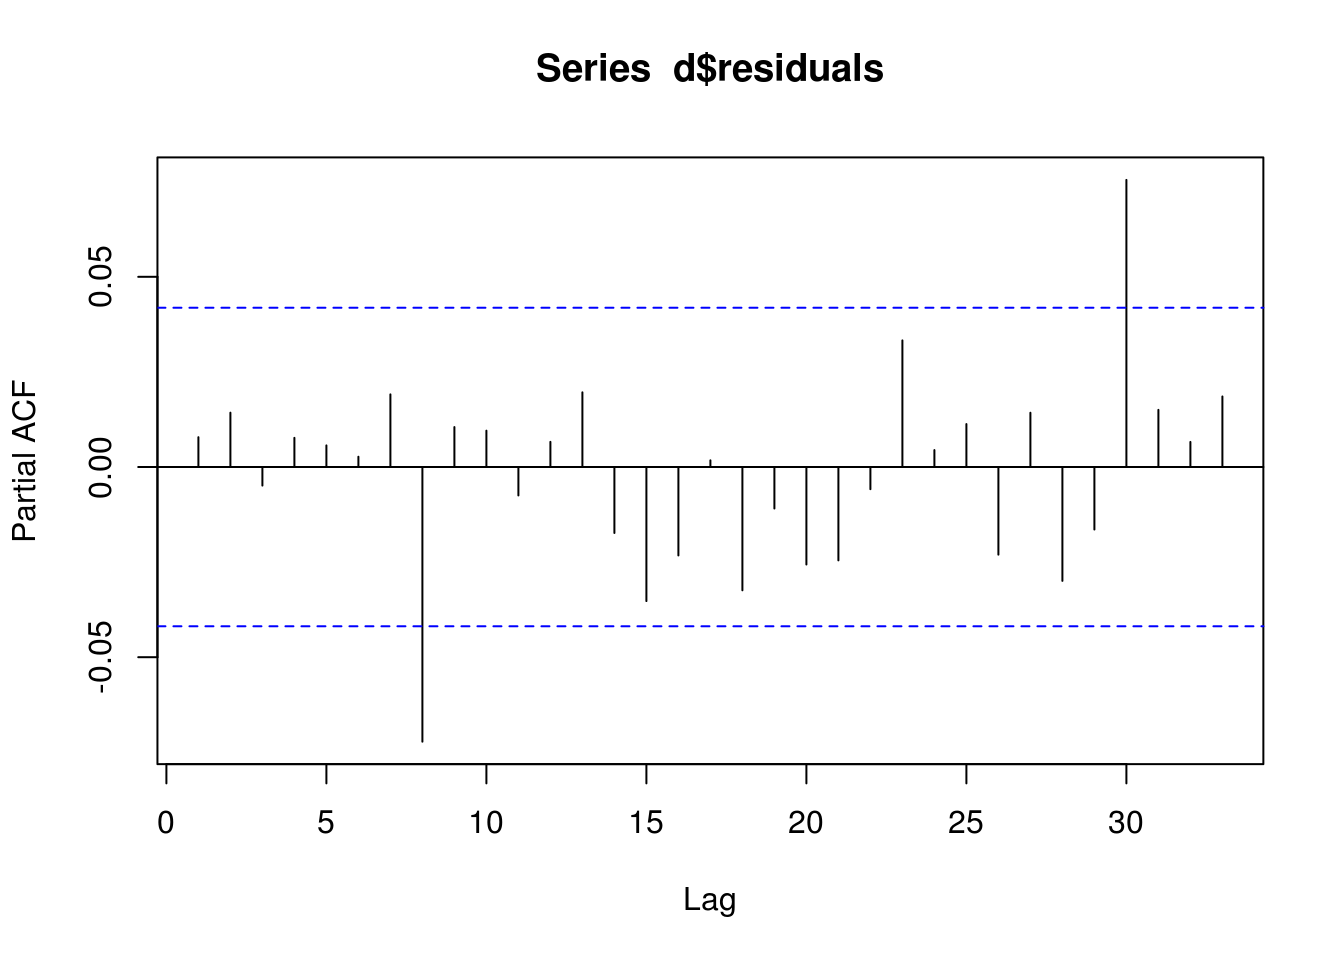
\includegraphics{website_files/figure-latex/unnamed-chunk-65-1.pdf}

\begin{Shaded}
\begin{Highlighting}[]
\KeywordTok{acf}\NormalTok{(d}\OperatorTok{$}\NormalTok{residuals)}
\end{Highlighting}
\end{Shaded}

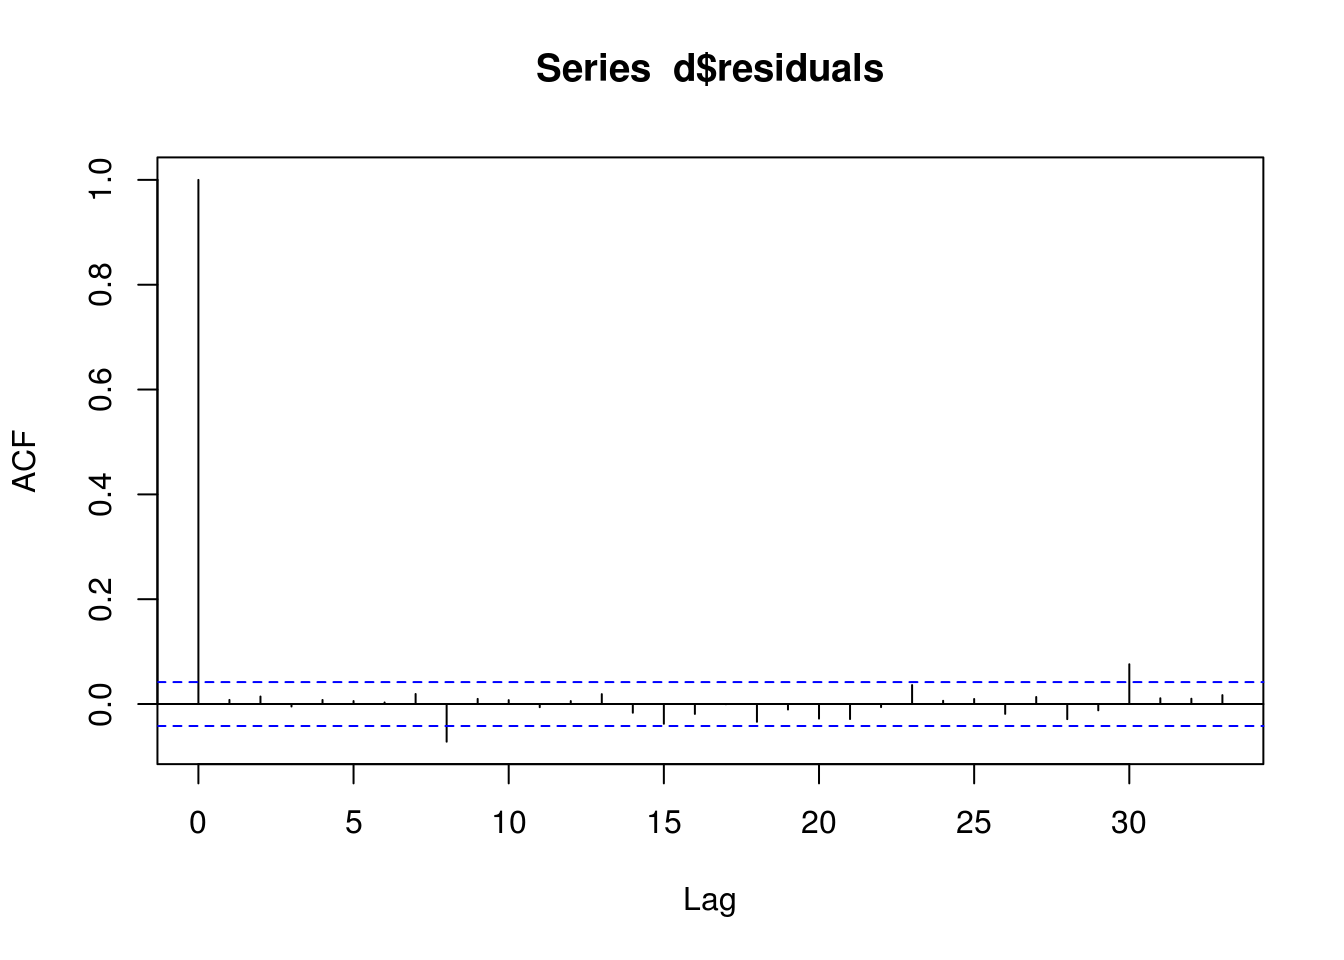
\includegraphics{website_files/figure-latex/unnamed-chunk-65-2.pdf}

\newpage

\section{Exercise 2}\label{exercise-2-1}

\begin{Shaded}
\begin{Highlighting}[]
\KeywordTok{library}\NormalTok{(data.table)}
\NormalTok{d <-}\StringTok{ }\KeywordTok{fread}\NormalTok{(}\StringTok{"data/exercise_2.csv"}\NormalTok{)}

\NormalTok{fit0 <-}\StringTok{ }\NormalTok{MASS}\OperatorTok{::}\KeywordTok{glmmPQL}\NormalTok{(y}\OperatorTok{~}\NormalTok{yearMinus2000 }\OperatorTok{+}\StringTok{ }\NormalTok{numberOfCows, }\DataTypeTok{random =} \OperatorTok{~}\StringTok{ }\DecValTok{1} \OperatorTok{|}\StringTok{ }\NormalTok{fylke,}
                \DataTypeTok{family =}\NormalTok{ poisson, }\DataTypeTok{data =}\NormalTok{ d)}
\end{Highlighting}
\end{Shaded}

\begin{verbatim}
## iteration 1
\end{verbatim}

\begin{verbatim}
## iteration 2
\end{verbatim}

\begin{Shaded}
\begin{Highlighting}[]
\NormalTok{fit1 <-}\StringTok{ }\NormalTok{MASS}\OperatorTok{::}\KeywordTok{glmmPQL}\NormalTok{(y}\OperatorTok{~}\NormalTok{season }\OperatorTok{+}\StringTok{ }\NormalTok{yearMinus2000 }\OperatorTok{+}\StringTok{ }\NormalTok{numberOfCows, }\DataTypeTok{random =} \OperatorTok{~}\StringTok{ }\DecValTok{1} \OperatorTok{|}\StringTok{ }\NormalTok{fylke,}
                \DataTypeTok{family =}\NormalTok{ poisson, }\DataTypeTok{data =}\NormalTok{ d)}
\end{Highlighting}
\end{Shaded}

\begin{verbatim}
## iteration 1
## iteration 2
\end{verbatim}

\begin{verbatim}
## iteration 3
\end{verbatim}

\begin{Shaded}
\begin{Highlighting}[]
\KeywordTok{print}\NormalTok{(lmtest}\OperatorTok{::}\KeywordTok{lrtest}\NormalTok{(fit0, fit1))}
\end{Highlighting}
\end{Shaded}

\begin{verbatim}
## Likelihood ratio test
## 
## Model 1: y ~ yearMinus2000 + numberOfCows
## Model 2: y ~ season + yearMinus2000 + numberOfCows
##   #Df LogLik Df Chisq Pr(>Chisq)
## 1   5                           
## 2   8         3
\end{verbatim}

\begin{Shaded}
\begin{Highlighting}[]
\KeywordTok{summary}\NormalTok{(fit1)}
\end{Highlighting}
\end{Shaded}

\begin{verbatim}
## Linear mixed-effects model fit by maximum likelihood
##  Data: d 
##   AIC BIC logLik
##    NA  NA     NA
## 
## Random effects:
##  Formula: ~1 | fylke
##         (Intercept) Residual
## StdDev:  0.08342256 1.298934
## 
## Variance function:
##  Structure: fixed weights
##  Formula: ~invwt 
## Fixed effects: y ~ season + yearMinus2000 + numberOfCows 
##                    Value  Std.Error   DF   t-value p-value
## (Intercept)    0.8483946 0.05053613 6565  16.78788  0.0000
## seasonSpring   0.9334080 0.00685147 6565 136.23480  0.0000
## seasonSummer   1.9312703 0.00621739 6565 310.62400  0.0000
## seasonWinter  -0.0822382 0.00841368 6565  -9.77434  0.0000
## yearMinus2000  0.2004222 0.00104237 6565 192.27503  0.0000
## numberOfCows   0.0005788 0.00077223 6565   0.74954  0.4536
##  Correlation: 
##               (Intr) ssnSpr ssnSmm ssnWnt yM2000
## seasonSpring  -0.097                            
## seasonSummer  -0.106  0.793                     
## seasonWinter  -0.079  0.586  0.646              
## yearMinus2000 -0.268  0.000  0.000 -0.002       
## numberOfCows  -0.070 -0.002 -0.018  0.004 -0.020
## 
## Standardized Within-Group Residuals:
##         Min          Q1         Med          Q3         Max 
## -5.44473503 -0.49365704 -0.05256441  0.39697143 16.32534219 
## 
## Number of Observations: 6573
## Number of Groups: 3
\end{verbatim}

\begin{Shaded}
\begin{Highlighting}[]
\NormalTok{d[,residuals}\OperatorTok{:}\ErrorTok{=}\KeywordTok{residuals}\NormalTok{(fit1, }\DataTypeTok{type =} \StringTok{"normalized"}\NormalTok{)]}

\KeywordTok{pacf}\NormalTok{(d}\OperatorTok{$}\NormalTok{residuals)}
\end{Highlighting}
\end{Shaded}

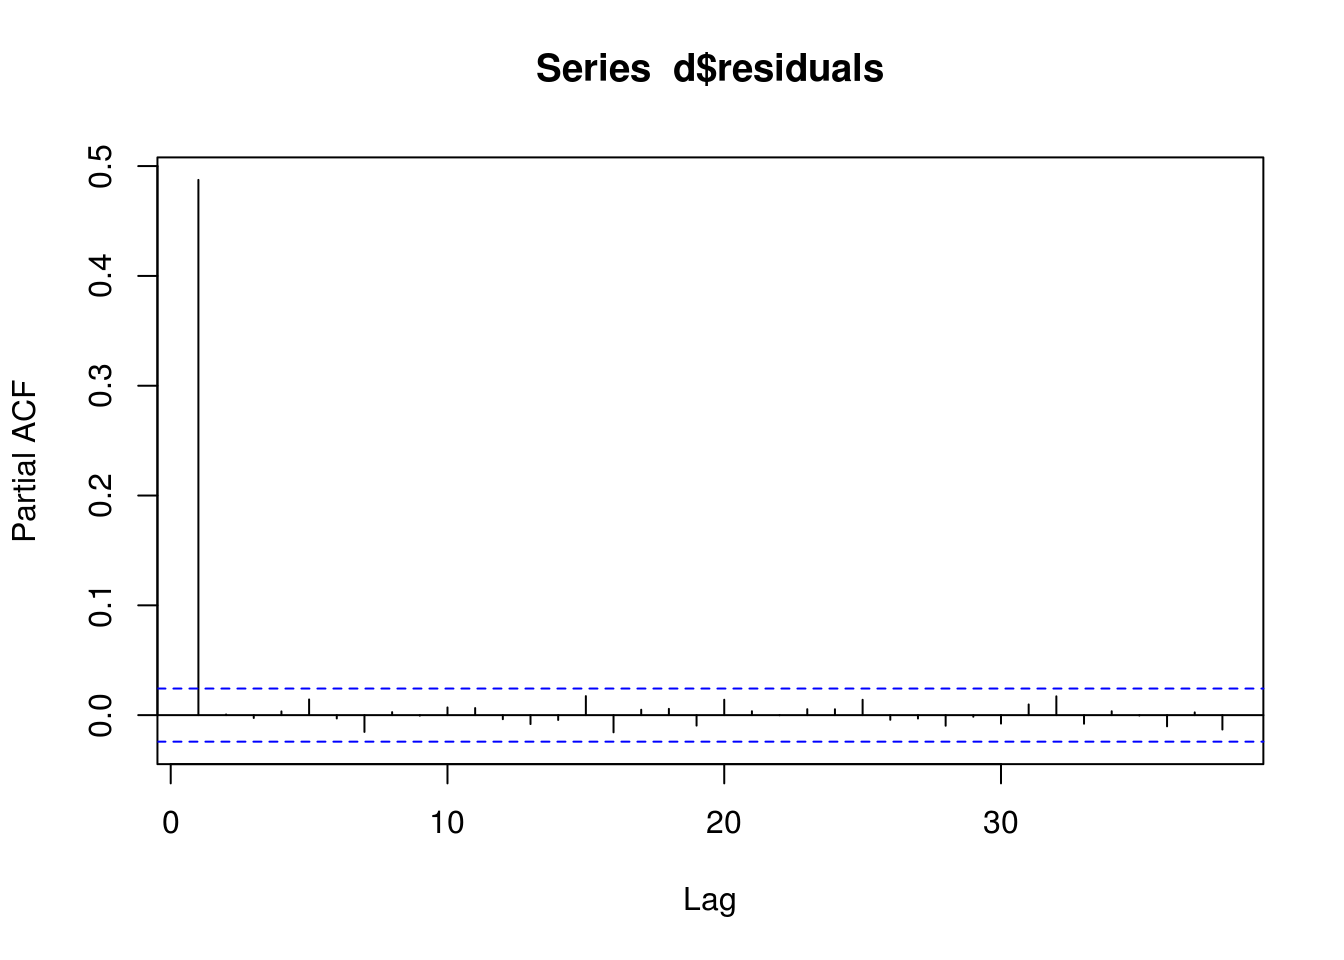
\includegraphics{website_files/figure-latex/unnamed-chunk-66-1.pdf}

\begin{Shaded}
\begin{Highlighting}[]
\KeywordTok{acf}\NormalTok{(d}\OperatorTok{$}\NormalTok{residuals)}
\end{Highlighting}
\end{Shaded}

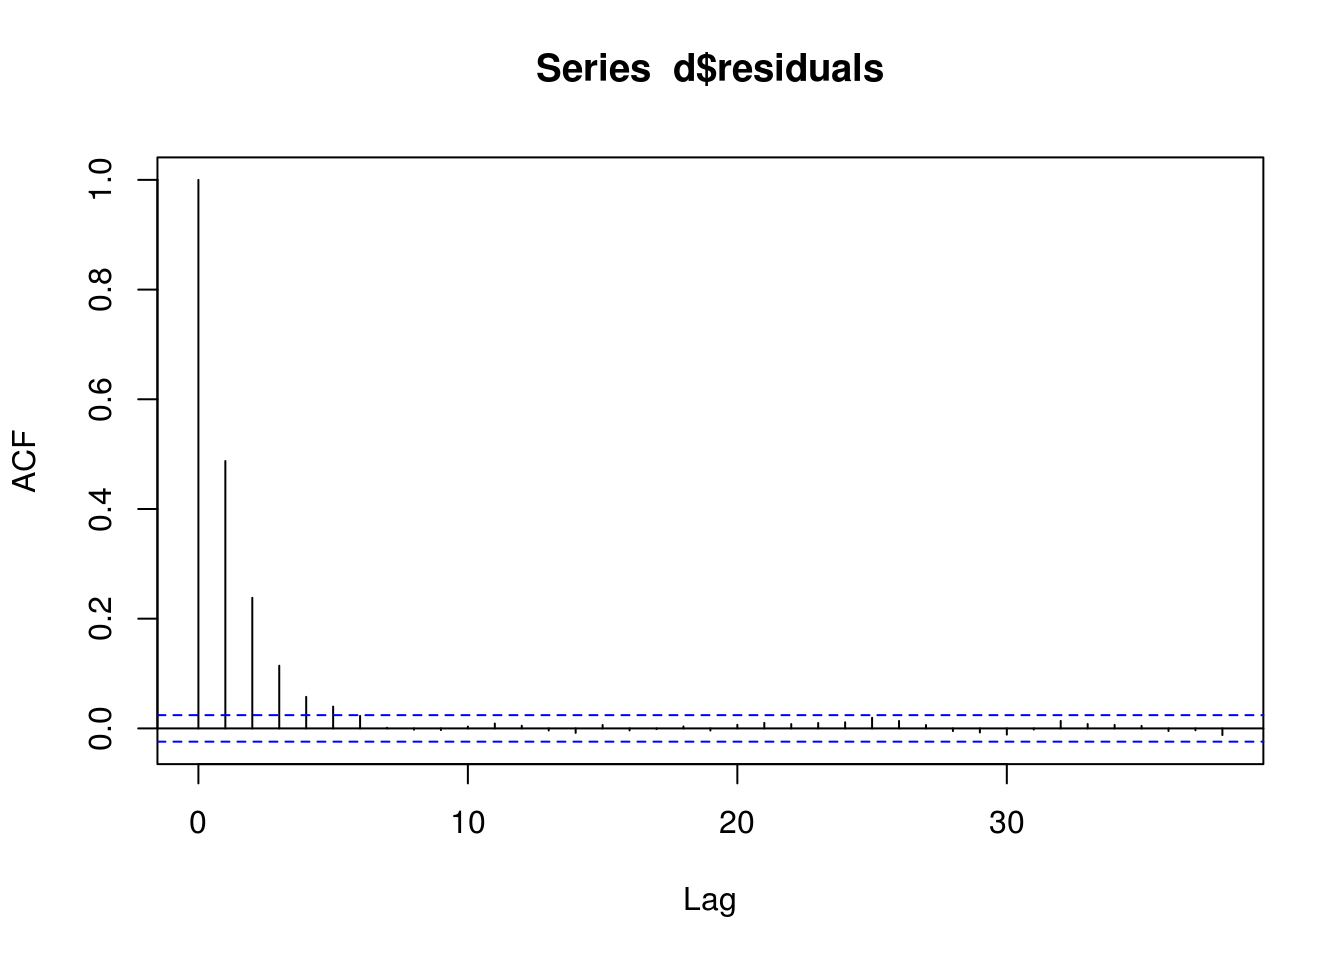
\includegraphics{website_files/figure-latex/unnamed-chunk-66-2.pdf}

\begin{Shaded}
\begin{Highlighting}[]
\NormalTok{fit1 <-}\StringTok{ }\NormalTok{MASS}\OperatorTok{::}\KeywordTok{glmmPQL}\NormalTok{(y}\OperatorTok{~}\NormalTok{season }\OperatorTok{+}\StringTok{ }\NormalTok{yearMinus2000 }\OperatorTok{+}\StringTok{ }\NormalTok{numberOfCows, }\DataTypeTok{random =} \OperatorTok{~}\StringTok{ }\DecValTok{1} \OperatorTok{|}\StringTok{ }\NormalTok{fylke,}
                \DataTypeTok{family =}\NormalTok{ poisson, }\DataTypeTok{data =}\NormalTok{ d,}
                \DataTypeTok{correlation=}\NormalTok{nlme}\OperatorTok{::}\KeywordTok{corAR1}\NormalTok{(}\DataTypeTok{form=}\OperatorTok{~}\NormalTok{dayOfSeries}\OperatorTok{|}\NormalTok{fylke))}
\end{Highlighting}
\end{Shaded}

\begin{verbatim}
## iteration 1
\end{verbatim}

\begin{verbatim}
## iteration 2
\end{verbatim}

\begin{verbatim}
## iteration 3
\end{verbatim}

\begin{Shaded}
\begin{Highlighting}[]
\KeywordTok{summary}\NormalTok{(fit1)}
\end{Highlighting}
\end{Shaded}

\begin{verbatim}
## Linear mixed-effects model fit by maximum likelihood
##  Data: d 
##   AIC BIC logLik
##    NA  NA     NA
## 
## Random effects:
##  Formula: ~1 | fylke
##         (Intercept) Residual
## StdDev:  0.08328798 1.319938
## 
## Correlation Structure: AR(1)
##  Formula: ~dayOfSeries | fylke 
##  Parameter estimate(s):
##       Phi 
## 0.5525116 
## Variance function:
##  Structure: fixed weights
##  Formula: ~invwt 
## Fixed effects: y ~ season + yearMinus2000 + numberOfCows 
##                    Value  Std.Error   DF   t-value p-value
## (Intercept)    0.9283222 0.05561940 6565  16.69062   0.000
## seasonSpring   0.8631442 0.01224757 6565  70.47476   0.000
## seasonSummer   1.8166993 0.01098229 6565 165.42086   0.000
## seasonWinter  -0.1394364 0.01488823 6565  -9.36554   0.000
## yearMinus2000  0.2001812 0.00197415 6565 101.40142   0.000
## numberOfCows   0.0004206 0.00057695 6565   0.72909   0.466
##  Correlation: 
##               (Intr) ssnSpr ssnSmm ssnWnt yM2000
## seasonSpring  -0.155                            
## seasonSummer  -0.171  0.784                     
## seasonWinter  -0.123  0.574  0.621              
## yearMinus2000 -0.464  0.000  0.000 -0.002       
## numberOfCows  -0.049  0.001 -0.006  0.004 -0.007
## 
## Standardized Within-Group Residuals:
##         Min          Q1         Med          Q3         Max 
## -5.03056012 -0.54478730 -0.04721577  0.46011628 15.05853958 
## 
## Number of Observations: 6573
## Number of Groups: 3
\end{verbatim}

\begin{Shaded}
\begin{Highlighting}[]
\NormalTok{d[,residuals}\OperatorTok{:}\ErrorTok{=}\KeywordTok{residuals}\NormalTok{(fit1, }\DataTypeTok{type =} \StringTok{"normalized"}\NormalTok{)]}

\KeywordTok{pacf}\NormalTok{(d}\OperatorTok{$}\NormalTok{residuals)}
\end{Highlighting}
\end{Shaded}

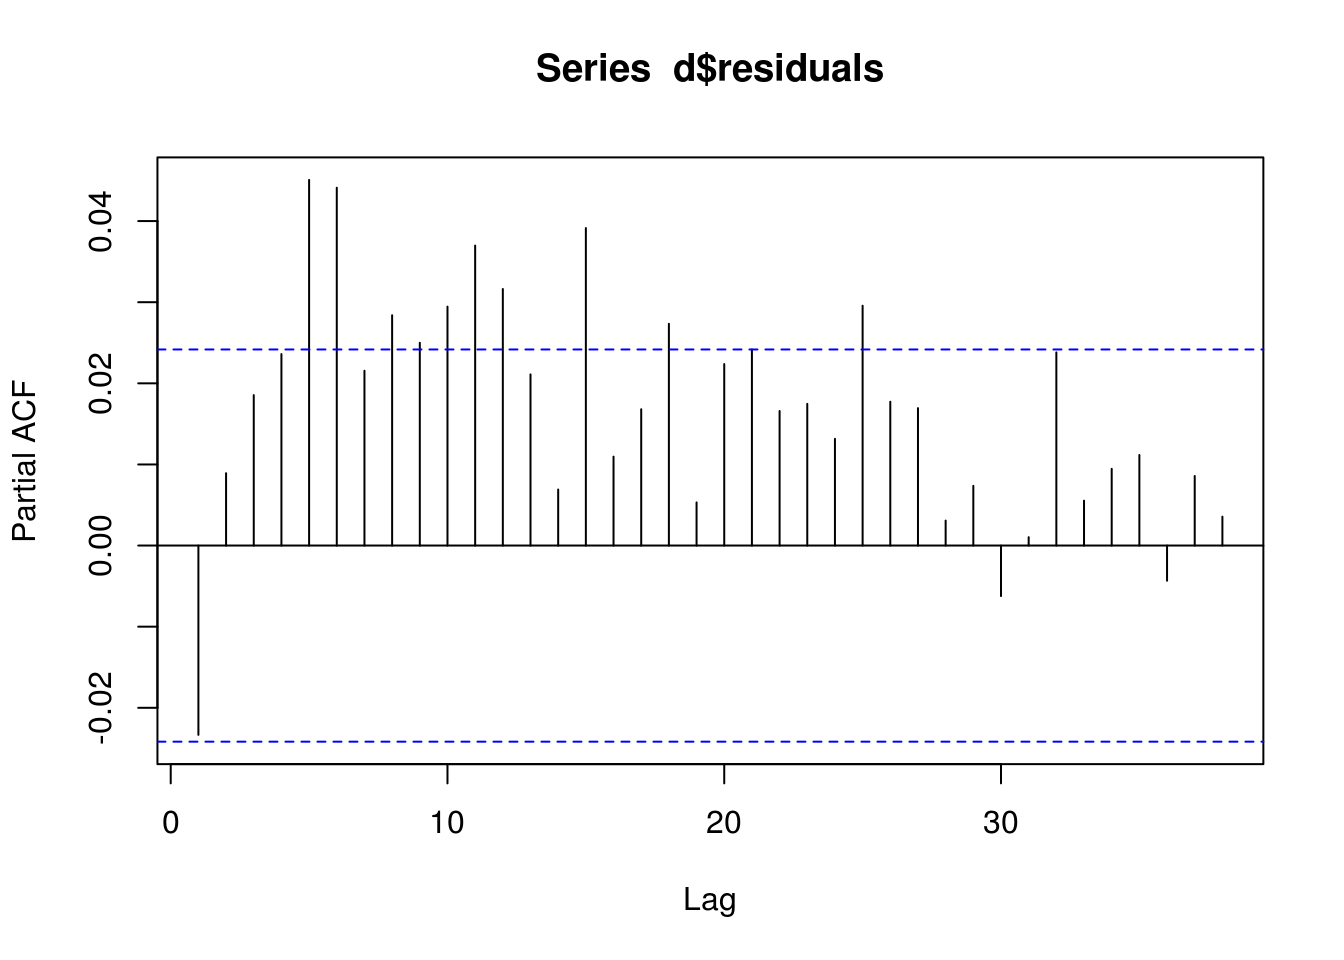
\includegraphics{website_files/figure-latex/unnamed-chunk-66-3.pdf}

\begin{Shaded}
\begin{Highlighting}[]
\KeywordTok{acf}\NormalTok{(d}\OperatorTok{$}\NormalTok{residuals)}
\end{Highlighting}
\end{Shaded}

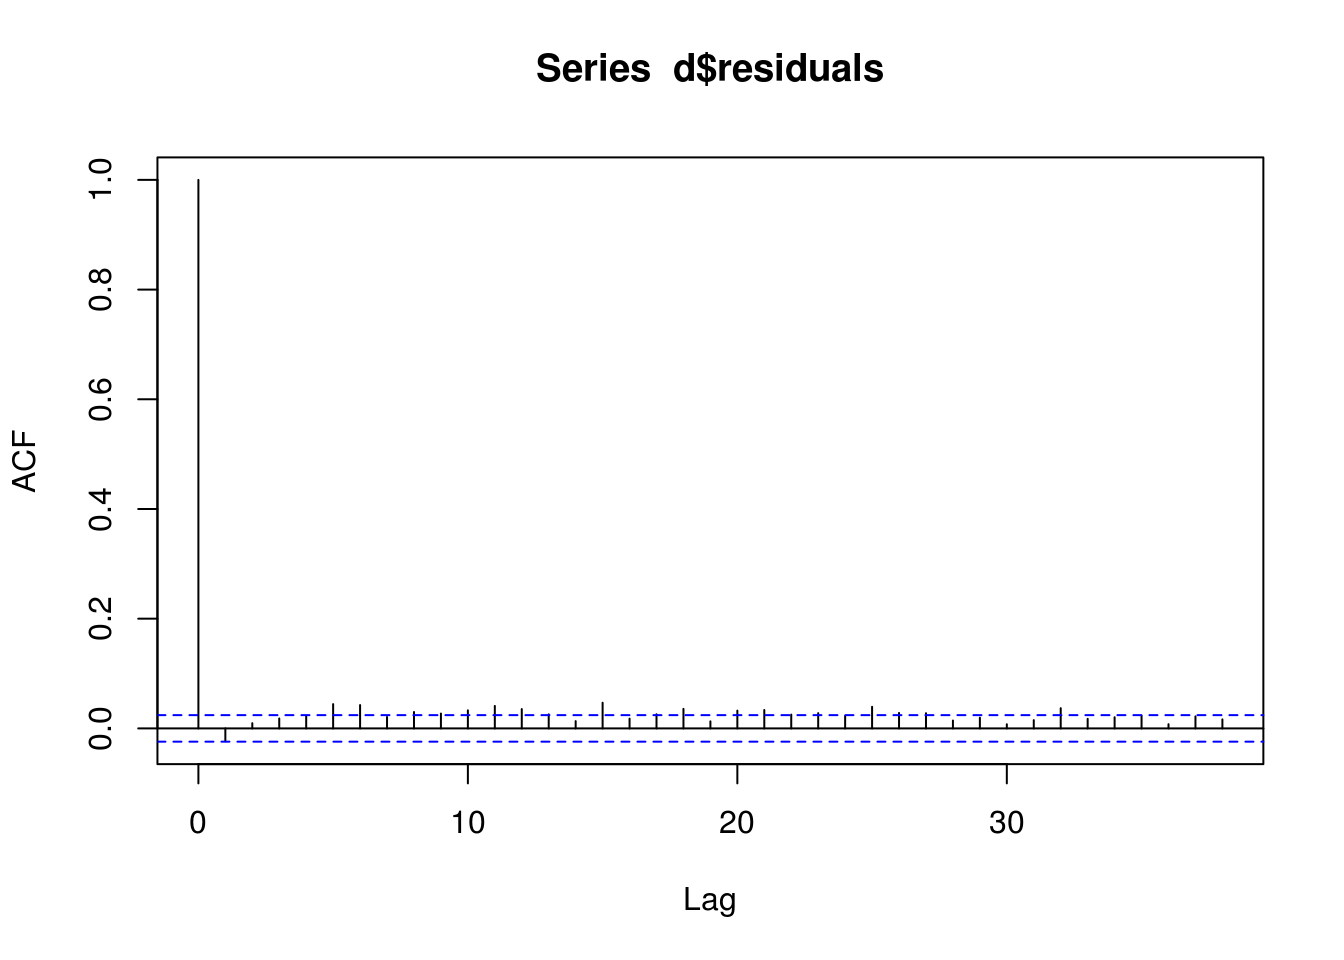
\includegraphics{website_files/figure-latex/unnamed-chunk-66-4.pdf}

\newpage

\section{Exercise 3}\label{exercise-3-1}

\begin{Shaded}
\begin{Highlighting}[]
\KeywordTok{library}\NormalTok{(data.table)}
\NormalTok{d <-}\StringTok{ }\KeywordTok{fread}\NormalTok{(}\StringTok{"data/exercise_3.csv"}\NormalTok{)}

\NormalTok{fit0 <-}\StringTok{ }\NormalTok{lme4}\OperatorTok{::}\KeywordTok{glmer}\NormalTok{(y }\OperatorTok{~}\StringTok{ }\NormalTok{yearMinus2000 }\OperatorTok{+}\StringTok{ }\NormalTok{numberOfCows }\OperatorTok{+}\StringTok{ }\NormalTok{(}\DecValTok{1}\OperatorTok{|}\NormalTok{fylke), }\DataTypeTok{family =}\NormalTok{ poisson, }\DataTypeTok{data =}\NormalTok{ d)}
\NormalTok{fit1 <-}\StringTok{ }\NormalTok{lme4}\OperatorTok{::}\KeywordTok{glmer}\NormalTok{(y }\OperatorTok{~}\StringTok{ }\NormalTok{season }\OperatorTok{+}\StringTok{ }\NormalTok{yearMinus2000 }\OperatorTok{+}\StringTok{ }\NormalTok{numberOfCows }\OperatorTok{+}\StringTok{ }\NormalTok{(}\DecValTok{1}\OperatorTok{|}\NormalTok{fylke), }\DataTypeTok{family =}\NormalTok{ poisson, }\DataTypeTok{data =}\NormalTok{ d)}
\end{Highlighting}
\end{Shaded}

\begin{verbatim}
## Warning in checkConv(attr(opt, "derivs"), opt$par, ctrl = control
## $checkConv, : Model failed to converge with max|grad| = 0.0013139 (tol =
## 0.001, component 1)
\end{verbatim}

\begin{Shaded}
\begin{Highlighting}[]
\KeywordTok{print}\NormalTok{(lmtest}\OperatorTok{::}\KeywordTok{lrtest}\NormalTok{(fit0, fit1))}
\end{Highlighting}
\end{Shaded}

\begin{verbatim}
## Likelihood ratio test
## 
## Model 1: y ~ yearMinus2000 + numberOfCows + (1 | fylke)
## Model 2: y ~ season + yearMinus2000 + numberOfCows + (1 | fylke)
##   #Df   LogLik Df Chisq Pr(>Chisq)    
## 1   4 -10144.4                        
## 2   7  -1794.9  3 16699  < 2.2e-16 ***
## ---
## Signif. codes:  0 '***' 0.001 '**' 0.01 '*' 0.05 '.' 0.1 ' ' 1
\end{verbatim}

\begin{Shaded}
\begin{Highlighting}[]
\KeywordTok{summary}\NormalTok{(fit1)}
\end{Highlighting}
\end{Shaded}

\begin{verbatim}
## Generalized linear mixed model fit by maximum likelihood (Laplace
##   Approximation) [glmerMod]
##  Family: poisson  ( log )
## Formula: y ~ season + yearMinus2000 + numberOfCows + (1 | fylke)
##    Data: d
## 
##      AIC      BIC   logLik deviance df.resid 
##   3603.8   3634.6  -1794.9   3589.8      593 
## 
## Scaled residuals: 
##     Min      1Q  Median      3Q     Max 
## -3.4683 -0.6176 -0.0064  0.5895  3.1431 
## 
## Random effects:
##  Groups Name        Variance Std.Dev.
##  fylke  (Intercept) 0.005643 0.07512 
## Number of obs: 600, groups:  fylke, 3
## 
## Fixed effects:
##                 Estimate Std. Error z value Pr(>|z|)    
## (Intercept)    0.0817819  0.0707498   1.156    0.248    
## seasonSpring   1.0213789  0.0246508  41.434   <2e-16 ***
## seasonSummer   2.0118660  0.0220035  91.434   <2e-16 ***
## seasonWinter  -0.0001082  0.0294244  -0.004    0.997    
## yearMinus2000  0.2019749  0.0038745  52.129   <2e-16 ***
## numberOfCows  -0.0045764  0.0028115  -1.628    0.104    
## ---
## Signif. codes:  0 '***' 0.001 '**' 0.01 '*' 0.05 '.' 0.1 ' ' 1
## 
## Correlation of Fixed Effects:
##             (Intr) ssnSpr ssnSmm ssnWnt yM2000
## seasonSprng -0.225                            
## seasonSummr -0.276  0.756                     
## seasonWintr -0.200  0.565  0.633              
## yearMns2000 -0.708 -0.020  0.008 -0.011       
## numberOfCws -0.200  0.025  0.038  0.053 -0.005
## convergence code: 0
## Model failed to converge with max|grad| = 0.0013139 (tol = 0.001, component 1)
\end{verbatim}

\bibliography{book.bib,packages.bib}


\end{document}
